\chapter{Time-Resolved Emittance Measurements}

Emittance is used as one of the main metrics to determine the quality of a charged particle beam.
Beam emittance determines the `focusability' of a beam which determines the size of the probe for electron and ion microscopes and is equivalent to the coherence of for synchrotrons, \glspl{xfel} and diffraction experiments.

Time-resolved measurements of emittance provide a powerful diagnostic for improvement of charged particle beams.
Elucidation of temporal emittance behaviour has the potential to permit better understanding of the processes involved in the creation and propagation of charged particle beam and thus could be a useful tool in improving these devices.
Time-resolved emittance has been performed previously using a pulsed \gls{mcp}~\cite{yoshida_simple_2001} and with optical transition radiation~\cite{le_sage_time-resolved_2002}.
This chapter presents a simple and novel method of measuring time-resolved emittance that is applicable to a wide range of charged particle sources and has the potential to be performed with a single-shot measurement.

The emittance of a \gls{caeis} is important to all of it's potential applications and the time-resolution provided by the technique described in this chapter will be a useful tool to examine the behaviour of the source and hopefully provide avenues for improvement.

Time resolved emittance measurements are useful {\color{red} (for what? check references for specific applications)} and have been achieved in a number of ways.
One method is to use a gated systems where the detector is only turned on for a short interval and the interval is adjusted from shot-to-shot to build up a temporal profile of the emittance measurement~\cite{bekefi_temporal_1987,yoshida_simple_2001}.
Another method is \gls{otr} which examines the radiation from a thin foil in order to determine the spatial profile and divergence of the particle beam and thus the emittance which has been time-resolved using a streak camera~\cite{fiorito_optical_1994}.
{\color{red}I don't really know how OTR works yet so I should read more or just not mention it.}

The method examined here for time-resolved emittance measurement is an adaption of the pepperpot methed that achieves the time resolution through streaking.
Streaking of charged particle beams involves applying a changing electric field to the beam in order to move it across the detector.
The streaking technique has been used previously for a number of measurements and is central to the operation of streak cameras.
Streaking has been used to provide time-resolution to ultrafast diffraction experiments using an rf deflecting cavity to $\sim$\unit[200][fs] resolution\cite{li_note:_2010}.
Streaked diffraction experiments have the potential to reveal dynamic information and due to the potential for single-shot measurements could be a useful tool on the road towards the `molecular movie'.

This chapter examines time-resolved emittance measurements through the streaking of pepperpots; including the theory involved, various technical considerations, example measurements and implementation of this technique with the \gls{caeis} at the University of Melbourne.


\section{Emittance}

A given ensemble of particles can be described by its density in six-dimensional phase space, $(x, p_x, y, p_x, z, p_z)$ where $(x, y, z)$ are the positions and $(p_x, p_y, p_z)$ are the momenta of each particle.
The extent of the beam in phase space is called the \emph{emittance}, $\epsilon$, of the beam.
Each cartesian direction is examined separately, $(\epsilon_x, x, p_x)$, $(\epsilon_y, y, p_y)$ and $(\epsilon_z, z, p_z)$ where $z$ is the optic axis of the beam.

Typically the gradients of trajectories in $x$-$z$ and $y$-$z$ are measured rather than the momenta.
These gradients are referred to as the divergence and are defined as
\begin{equation}\label{equation:divergence}
x^\prime \equiv \frac{dx}{dz} = \frac{v_x}{v_z}.
\end{equation}
The space of $(x, x^\prime)$ is referred to as trace-space.
An example of the trace-space occupied by a beam is shown in Figure~\ref{figure:emittance_example}.
The \emph{emittance} can be defined as
\begin{equation}
\epsilon^x \equiv \frac{A^x}{\pi}
\end{equation}
where $A^x$ is the area occupied by the beam in trace space.

\begin{figure}
\center
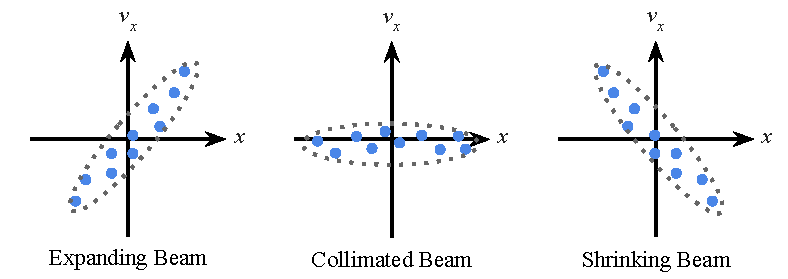
\includegraphics{part2/Figs/EmittanceExample.pdf}
\caption{An example of the trace-space occupied by an expanding, collimated and shrinking beam. The dotted line indicates the area occupied by the beam, the emittance.}
\label{figure:emittance_example}
\end{figure}

The density, $\rho$, of a beam of $N$ particles in trace space can usually be described by a Gaussian:
\begin{equation}\label{trace_space_density}
\rho(x, x^\prime) = N exp\left[ \frac{-(\sigma_{22}x^2-2\sigma_{12}xx^\prime+\sigma_{11}x^{\prime2}}{2|\sigma|} \right]
\end{equation}
where $|\sigma|$ is the determinant of the symmetric beam matrix,
\begin{equation}
\sigma = \begin{pmatrix} \sigma_{11} & \sigma_{12} \\ \sigma_{21} & \sigma_{22} \end{pmatrix}.
\end{equation}
$\sigma_{11}$ is the standard deviation of $x$, $\sigma_{22}$ the standard deviation of $x^\prime$ and $\sigma_{12}=\sigma_{21}$ indicates the coupling between $x$ and $x^\prime$. The \emph{emittance} can also be defined as
\begin{equation}\label{eq:emittancewithdeterminant}
\epsilon^x \equiv \sqrt{|\sigma|} = \sqrt{\sigma_{11}\sigma_{22}-\sigma_{12}^2}
\end{equation}

The \emph{\gls{rms} emittance} is a more practical measure and is defined as
\begin{equation}\label{emittance}
\epsilon \equiv \sqrt{\langle x^2\rangle \langle x^{\prime 2}\rangle - \langle x x^\prime\rangle^2}.
\end{equation}

The emittance of a beam represents the `focusability' of the beam.
A low emittance beam can be focused to a small waist than a high emittance beam, in fact a beam with zero emittance could be focused to a point whereas any beam with non-zero emittance has a finite spot size, this is shown in Figure~\ref{figure:focusability}.
This makes emittance an important quantity to consider in almost all beam applications but is particularly important to charged beams due to space-charge repulsion.

\begin{figure}
\center
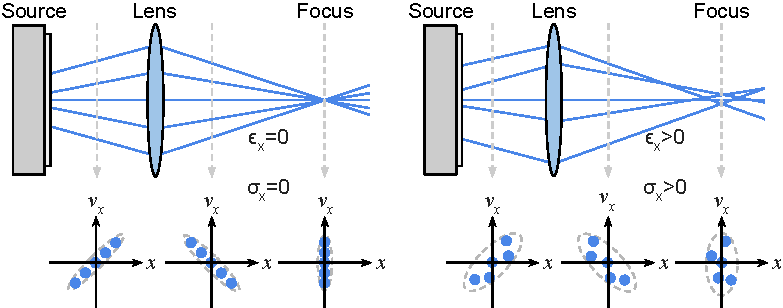
\includegraphics{part2/Figs/EmittanceFocasability.pdf}
\caption{On the left is a particle beam with zero emittance, and thus can be focused to a beam waist of zero width. On the right is a beam with non-zero emittance and thus a non-zero beam waist. Below each figure are plots of the phase space at difference points in the beam where the dashed line is indicitive of the phase-space area or emittance.}
\label{figure:focusability}
\end{figure}

\subsection{Emittance with a \gls{caeis}}
\label{section:excess_energy_emittance}

For a \gls{caes} the emittance at the source is given by~\cite{mcculloch_high-coherence_2013}
\begin{equation}\label{equation:excess_energy_emittance}
\epsilon_r = \sigma_r \sqrt{\frac{k_B T}{m_e c^2}}
\end{equation}

Discuss excess energy, realation to emittance, coherence etc.

\section{Measurement}

Directly calculating the emittance of an ensemble with Equation~\ref{emittance} requires full knowledge of the position and momenta of the particles which is difficult as beam monitors tend to only measure the transverse positions of particles.
There are a number of methods to practically calculate the emittance of a particle beam, namely pepperpots, the multiple profile method methods and the quadrupole method.

\subsection{Pepperpots}

The pepperpot method uses a beam mask, consisting of an array of small holes, to obscure the beam which is then propagated and detected downstream.
by examining the size of the spots on the detector the divergence of the beam can be estimated and thus the emittance of the beam can be calculated.
Ideally the extent of the array should be larger than the size of the beam and the holes are as small as is practical while maintaining sufficient flux and ensuring the spots on the detector do not overlap.
The name refers to the similarity of the simplest beam mask to the perforated lid of a container for pepper.

A useful derivation of this technique is presented in Ref.~\cite{zhang_emittance_1996} with the one dimensional result:

\begin{dmath}\label{equation:pepperpot}
\epsilon_x^2 = \left\langle x^2\right\rangle \left\langle x^{\prime2}\right\rangle - \left\langle xx^\prime\right\rangle^2\allowbreak
\approx \frac{1}{N^2} \left\{\left[\sum_{j=1}^p{n_j\left(x_{sj}-\bar{x}\right)^2}\right] \left[ \sum_{j=1}^p{\left[n_j\sigma_{x_j^\prime}^2 + n_j\left(\bar{x_j^\prime}-\bar{x^\prime}\right)^2\right]}\right] - \left[ \sum_{j=1}^p{n_jx_{sj}\bar{x_j^\prime}-N\bar{x}\bar{x^\prime}}\right]^2\right\}
\end{dmath}
where;
\begin{itemize}
    \item $N$ is the total number of particles after the beam mask,
    \item $p$ is the total number of holes in the $x$ direction,
    \item $n_j$ is the number of particles passing through the $j$-th hole and hitting the detector,
    \item $x_{sj}$ is position of the $j$-th hole,
    \item $\bar{x}$ is the mean position of the holes,
    \item $\sigma_{x_j^\prime}$ is the \gls{rms} divergence of the $j$-th beamlet,
    \item $\bar{x_j^\prime}$ is the mean divergence of the $j$-th beamlet, and
    \item $\bar{x^\prime}$ is the mean divergence of all beamlets.
\end{itemize}

An example pepperpot mask and detected beamlets are shown in Figure~\ref{figure:pepperpot_example}.
This equation can be implemented by appropriately rotating the detected beamlets and then performing row and column sums of the pixels followed by application of Equation~\ref{equation:pepperpot} for $x$ and $y$.

\begin{figure}
    \centering
    \begin{subfigure}{0.49\linewidth}
    \centering
    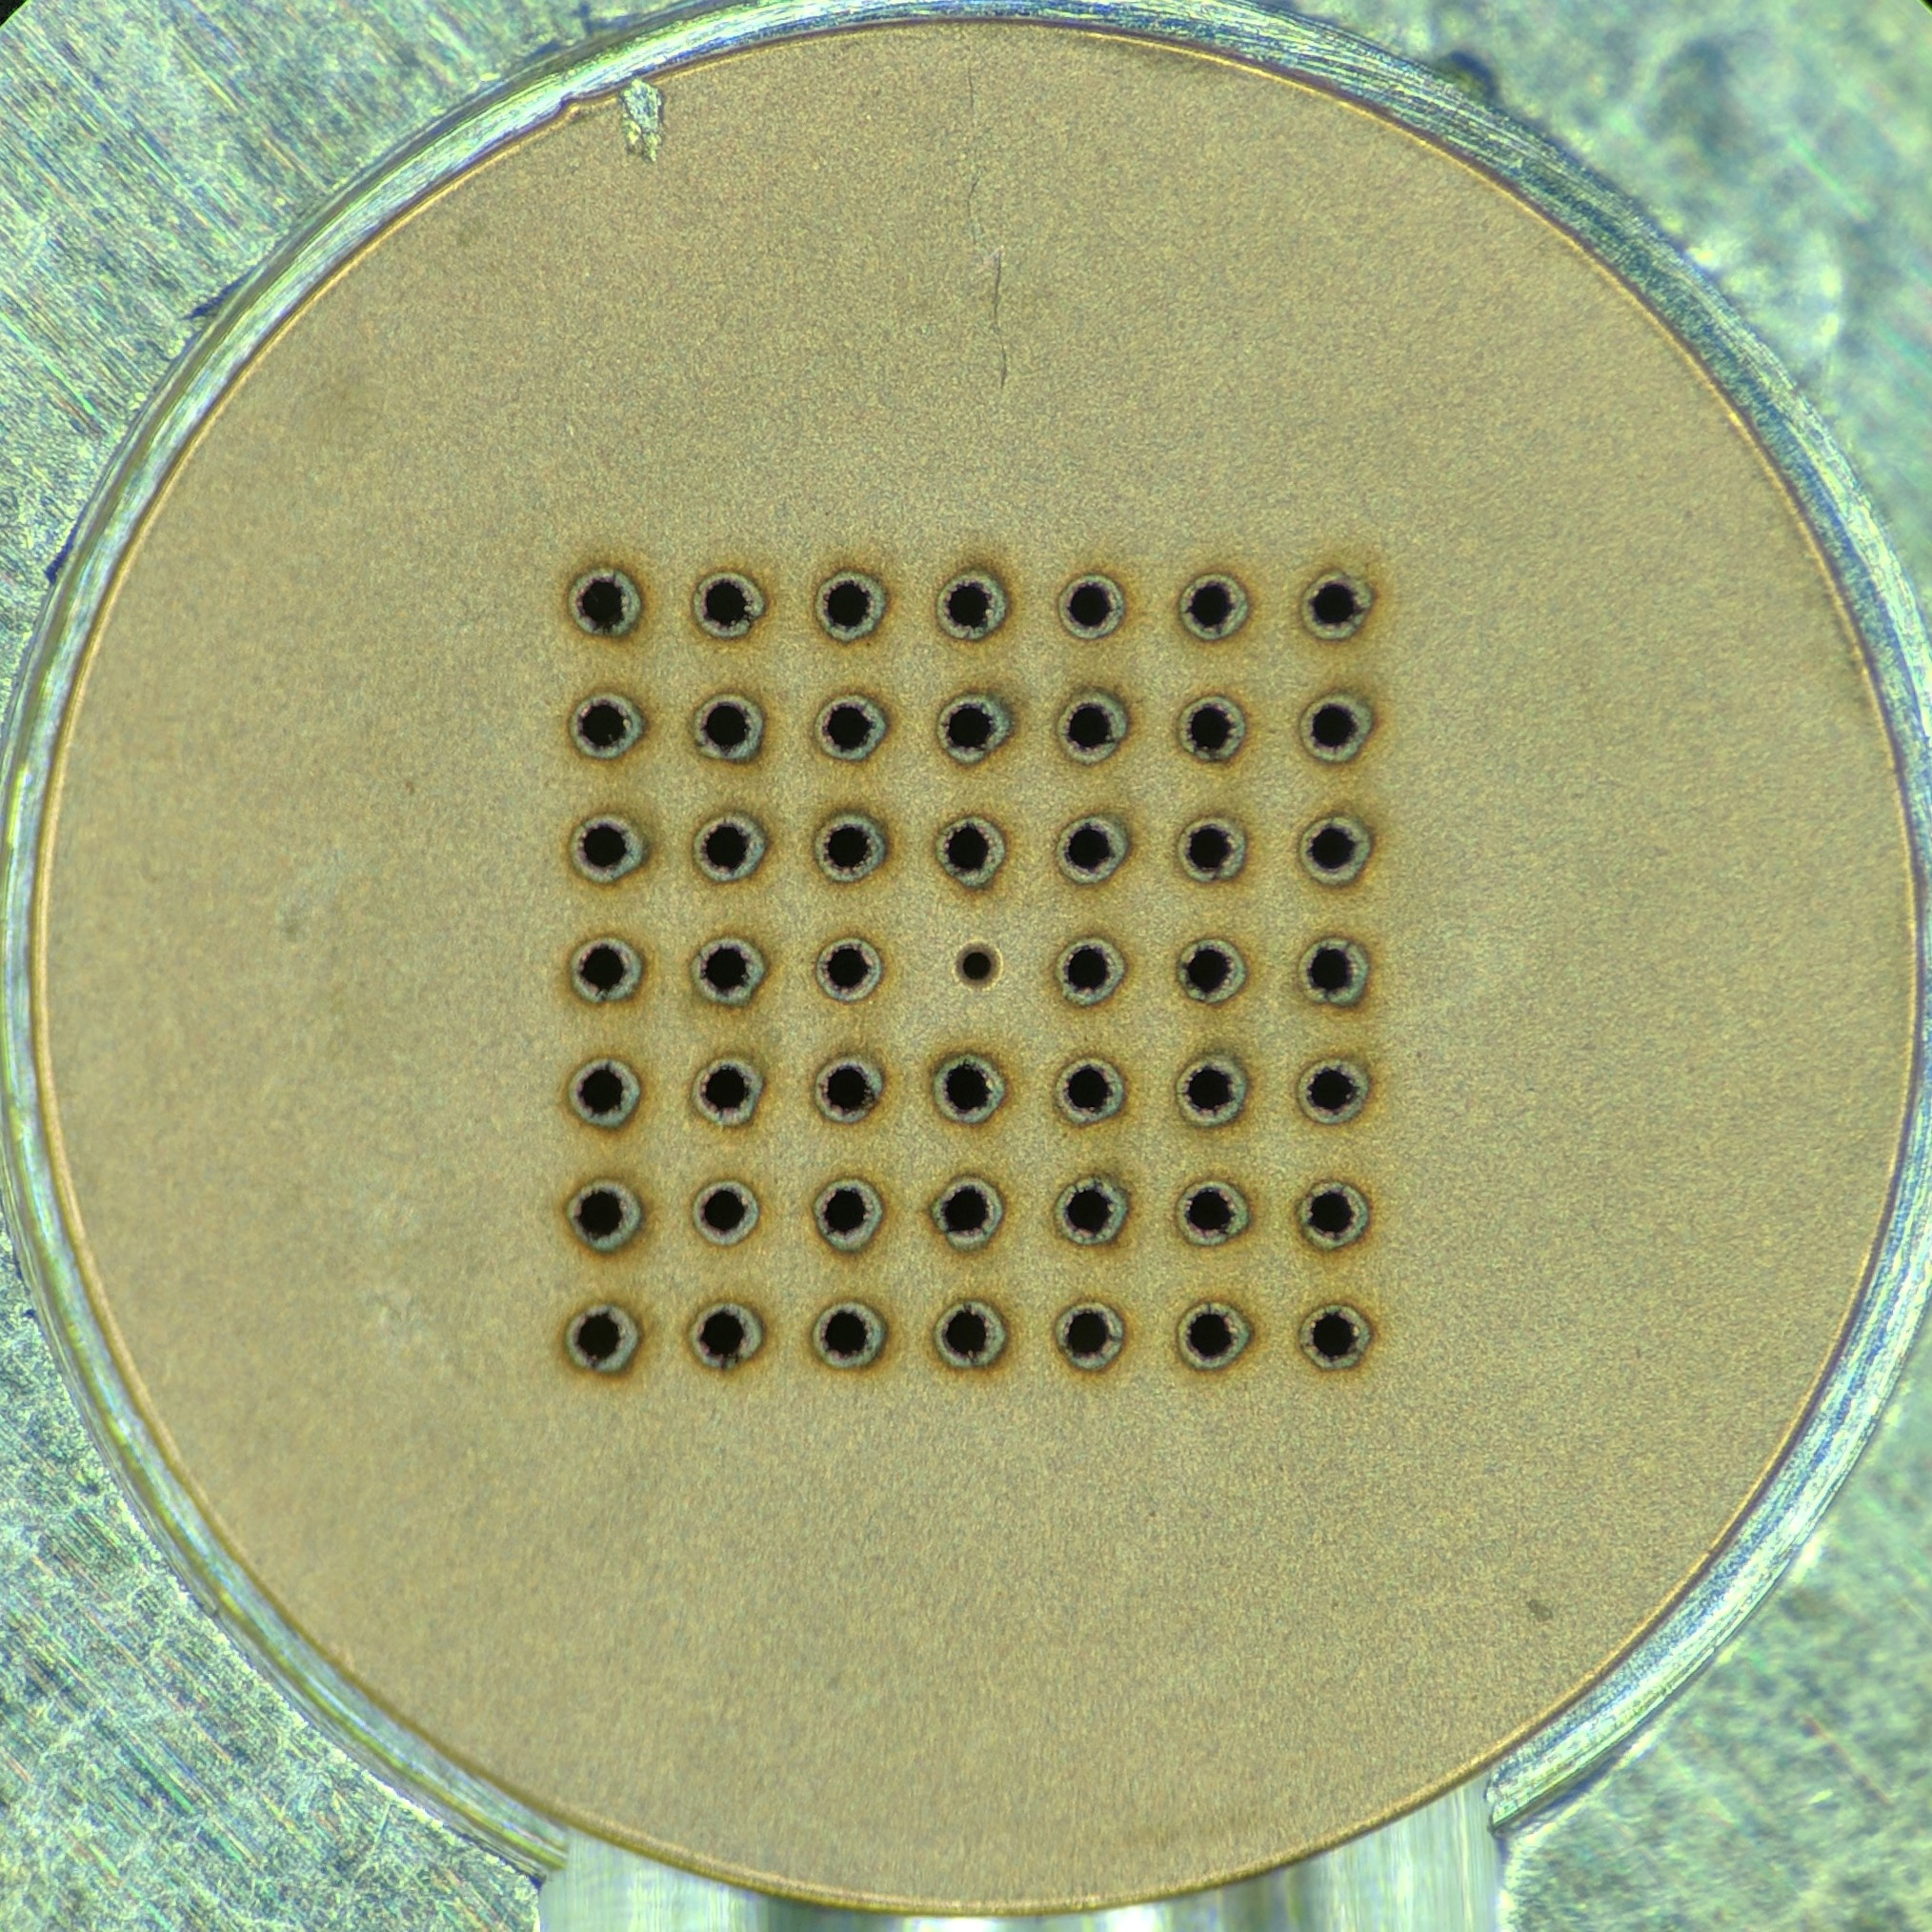
\includegraphics[width=\linewidth]{part2/Figs/example_pepperpot_mask.jpg}
    \caption{}
    \label{figure:pepperpot_mask}
    \end{subfigure}
    \begin{subfigure}{0.49\linewidth}
    \centering
    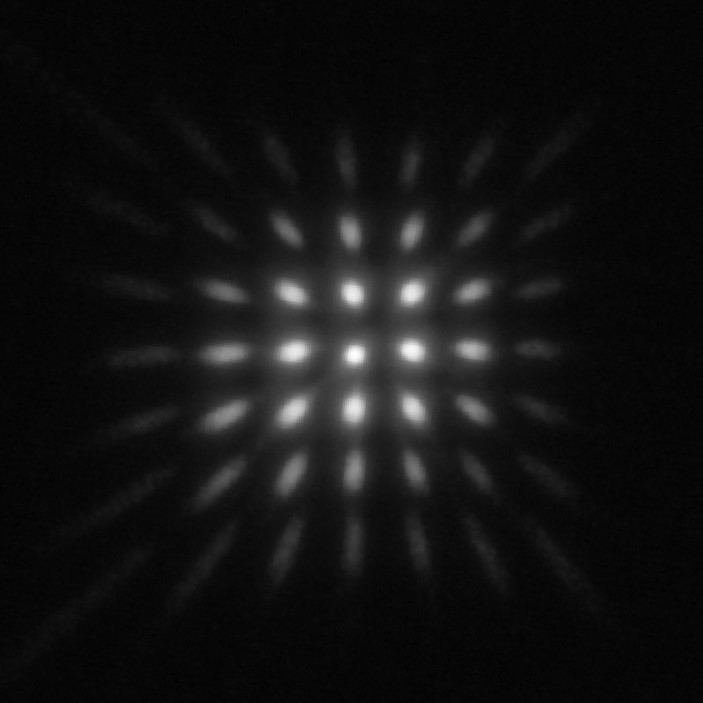
\includegraphics[width=\linewidth]{part2/Figs/example_pepperpot_detector_linear.jpeg}
    % 486.971 pepperpot from 2017.06.06
    \caption{}
    \label{figure:pepperpot_image}
    \end{subfigure}
    
    \begin{subfigure}{0.49\linewidth}
    \centering
    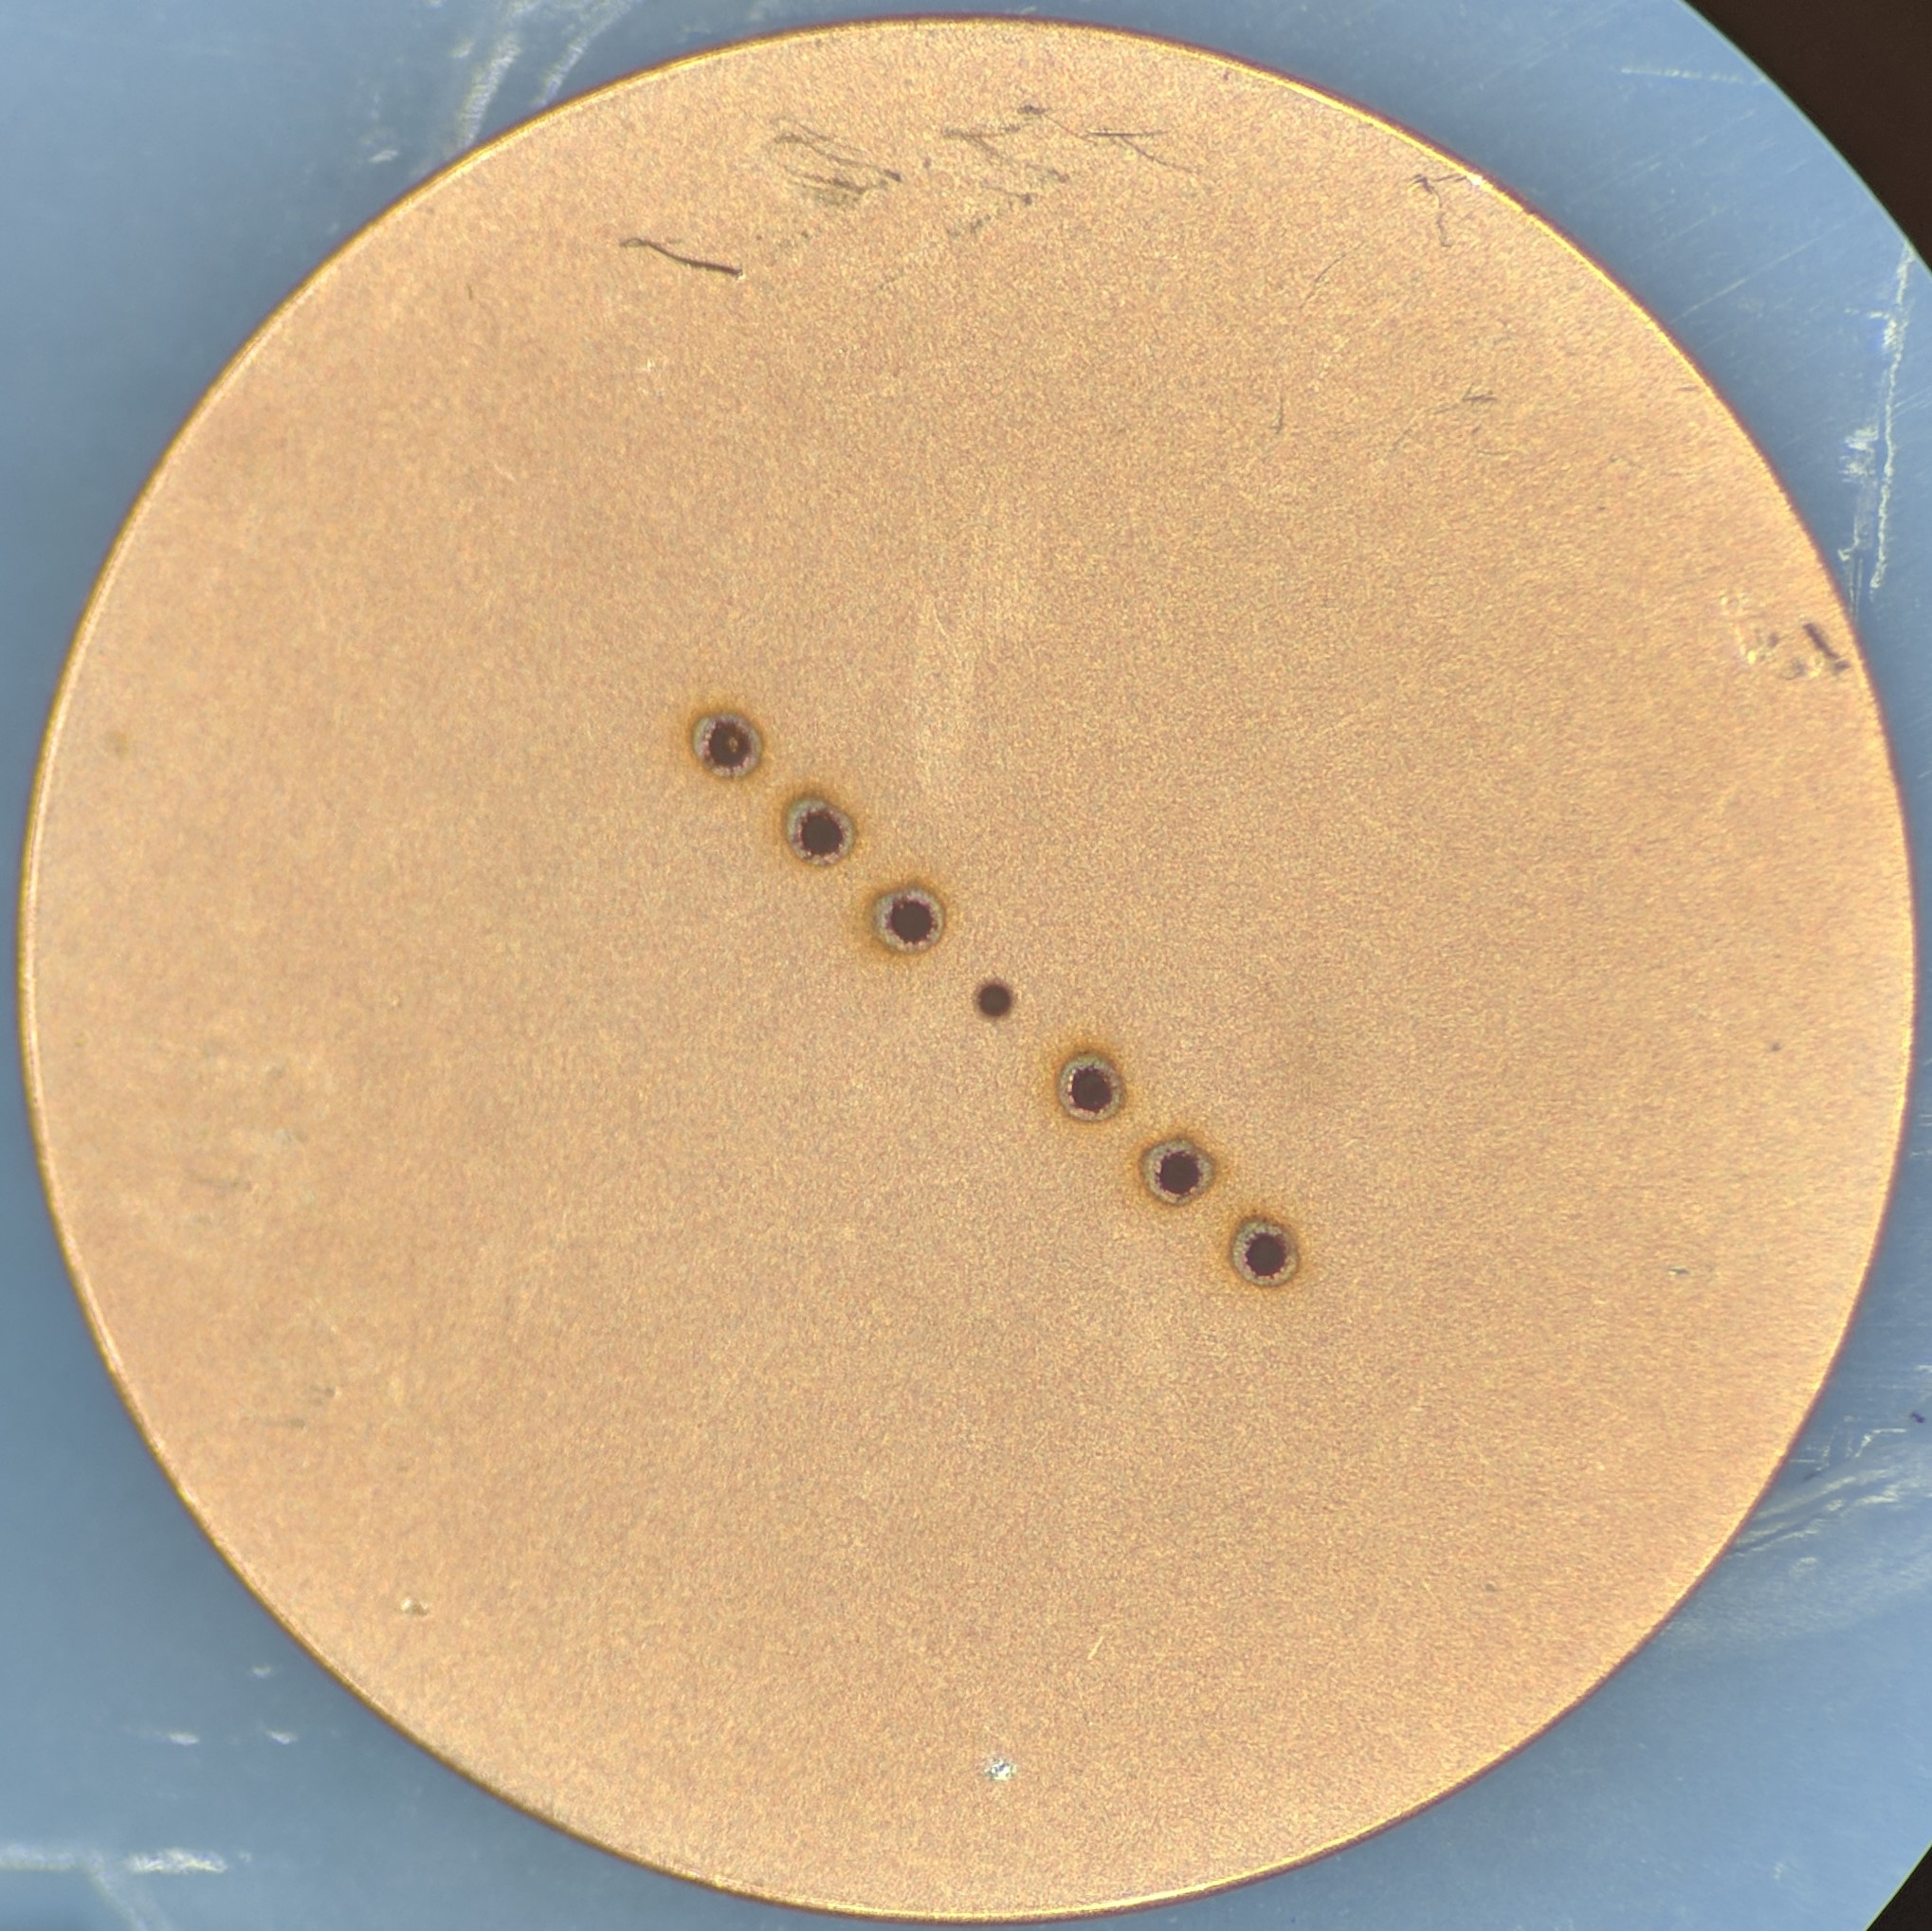
\includegraphics[width=\linewidth]{part2/Figs/example_pepperpot_1d.jpg}
    \caption{}
    \label{figure:1d_pepperpot}
    \end{subfigure}
    \begin{subfigure}{0.49\linewidth}
    \centering
    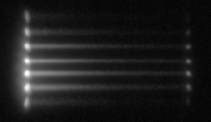
\includegraphics[width=\linewidth]{part2/Figs/example_streaked_pepperpot.png}
    \caption{}
    \label{figure:streaked_1d_pepperpot}
    \end{subfigure}
    % Manual labels.....
    \caption{(a) a pepperpot mask cut into a thing copper disk and, (b), the corresponding set of beamlets on the detector. (c) a one-dimensional pepperpot mask (held in place by a copper ring) and the corresponding streaked set of beamlets on the detector, (d). The beam images are log scaled.}
    \label{figure:pepperpot_example}
\end{figure}

\subsubsection{Temporal Resolution with Streaking}
A one-dimensional pepperpot cosists of either a line of holes or a line of slits and a line of holes is a prime target for a streaking measurement.
In this case streaking is performed with a time varying electric field which deflects the charged particles across the detector providing time-resolution.
For a pulsed charged particle source, such as the \gls{caeis}, the streak can be performed over the duration of the bunch or over a portion of the bunch if higher resolution is required.
There are some considerations for how fast an electric field can be swept, which will not be examined in detail here, so extremely short bunches will require more complicated systems, such as a rf-cavity, to provide the appropriate timing and electric field temporal-gradient~\cite{alesini_rf_2006}.
An example of a streaked pepperpot measurement is shown in Figure~\ref{figure:streaked_1d_pepperpot}.

\subsection{Multi-profile Method}

If a beam can be described by $\sigma^0$ at $z_0$ and by $\sigma^1$ at $z_1$ then the transformation matrix, $\mathbf{R}_{12}$ from $z_0$ to $z_1$ is
\begin{equation}
\mathbf{R} = \begin{pmatrix} R_{11} & R_{12} \\ R_{21} & R_{22} \end{pmatrix}
\end{equation}
and
\begin{equation}
\sigma^1 = \mathbf{R}\sigma^0\mathbf{R}^T
\end{equation}
where $\mathbf{R}^T$ is the transpose of $\mathbf{R}$.
The combined transfer matrix for a series of $z$ positions is simply the product of the individual transfer matrices.

We can write:
\begin{equation}\label{equation:multiprofile}
\sigma_{11}^1 = R_{11}^2\sigma_{11}^0 + 2R_{11}R_{12}\sigma_{12}^0 + R_{12}^2\sigma_{22}^0
\end{equation}

Typical detectors are only able to measure the standard deviation of $x$, $\sigma_{11}$.
With at least three measurements and known transfer matrices the other elements of $\sigma$ can be determined.
With more than three measurements uncertainty can be reduced.

The transfer matrix for simple propagation over a distance $L$ is
\begin{equation}
\mathbf{R}_L = \begin{pmatrix}1 & L \\ 0 & 1\end{pmatrix}
\end{equation}
and then Equation~\ref{equation:multiprofile} becomes
\begin{equation}
\sigma_{11}^1 = \sigma_{11}^0 + 2L \sigma_{12}^0 + L_1^2\sigma_{22}^0.
\end{equation}

\begin{figure}
\center
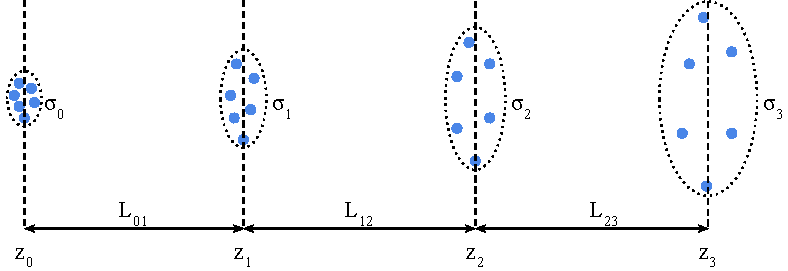
\includegraphics{part2/Figs/Multi-ProfileEmittance.pdf}
\caption{An example of a multi-profile emittance measurement conducted on an expanding beam travelling from left to right (or a shrinking beam travelling right to left).}
\label{figure:multiprofileexample}
\end{figure}

With an initial beam, $\sigma_0$, measured at $z_1, z_2$ and $z_3$ as shown in Figure~\ref{figure:multiprofileexample} then $\sigma_{11}^1$, $\sigma_{11}^2$, and $\sigma_{11}^3$ are know and we can write 
\begin{align}
\sigma_{11}^1 &= \sigma_{11}^0 +2L_{01}\sigma_{12}^0 + L_{01}^2\sigma_{22}^0 \notag\\
\sigma_{11}^2&= \sigma_{11}^0+2(L_{01}+L_{12})\sigma_{12}^0 + (L_{01}+L_{12})^2\sigma_{22}^0 \notag\\
\sigma_{11}^3&= \sigma_{11}^0+2(L_{01}+L_{12}+L_{23})\sigma_{12}^0 + (L_{01}+L_{12}+L_{23})^2\sigma_{22}^0 \label{eq:multiprofilesolution}
\end{align}

Which can easily be solved for $\sigma_0$ thus allowing the calculation of the emittance with Equation~\ref{eq:emittancewithdeterminant}.

This method is feasible with the \gls{caeis} at the University of Melbourne but labourious due to the manual operation of the bellows the detector is attached to.

\subsection{Quadrupole Method}

The quadrupole method is similar to the multi-profile method but requires only a single location to measure the beam width and a well characterised variable lens such as a quadrupole lens.
A quadrupole lens with a magnetic field gradient of $G$ has the transfer matrix in the focusing plane of
\begin{equation}
\mathbf{R}_f = \begin{pmatrix} \cos kl & (1/k)\sin kl\\
-k\sin kl & cos kl\end{pmatrix},
\end{equation}
where $l$ is the effective length of the quadrupole, $k^2=G/B\rho$ is the quadrupole strength and $B\rho$ is the magnetic rigidity of the particles in the assumed central trajectory.
The matrix in the defocusing palne is
\begin{equation}
\mathbf{R}_d = \begin{pmatrix} \cosh kl & (1/k) \sin kl\\
k \sinh kl & \cosh kl \end{pmatrix}
\end{equation}

A beam measured a distance $L$ away from the quadrupole will have undergone the transformation $\mathbf{R}=\mathbf{R}_L\mathbf{R}_f$ on one axis and $\mathbf{R}=\mathbf{R}_L\mathbf{R}_d$ on the other.
The symmetric beam matrix for the beam before the lens can then be determined from a series of beam profile measurements with different focusing strengths.
The main advantage of this measurement is that is only requires a single beam monitor location.

Due to the ad-hoc nature of the magnetic lenses used in the \gls{caes} this method is not practical without a thorough characterisation of the lenses, especially in comparison with the ease of the alternative methods.

\section{Simulation}

I didn't really do much simulation..... Remove this section? Or do some simulations.


\subsection{Pepperpots}

\subsection{Multiple Profile Method}

\subsection{Quadrupole Method}

\subsection{Streaking}

\subsubsection{Electron Energy}

Measurement resolution


Spot size


Stability/wrangling difficulty.


\subsubsection{Flux}

This is useful to know.
How much flux is required to get single shot measurements?
How does this match up to other charged particle sources?

\subsection{Measurement Resolution}

May be covered in other sections.


\section{Experimental Setup}

A number of modifications were made to the \gls{caeis} to prepare it for the streaked emittance measurements and there were a number of restrictions on various parameters due to the precise setup of the apparatus.
The \gls{caeis} was operated in electron mode for these measurements due to the available magnetic optics and the larger emittance expected from electrons as the source temperature is higher for electrons, a minimum temperature of approximately \unit[10]{K} for electrons and \unit[100]{$\mu K$} for ions~\cite{mcculloch_arbitrarily_2011}.
Using electrons also allows some control of the bunch emittance as the excess energy can be controled with the blue ionisation laser wavelength, with ions the change in emittance would be negligible.

See Chapter~\ref{chapter:setup} for a more detailed description of the \gls{caeis} and Figure~\ref{figure:emittance_schematic} for a schematic of the setup used for the measurements in this chapter.

\begin{figure}
\center
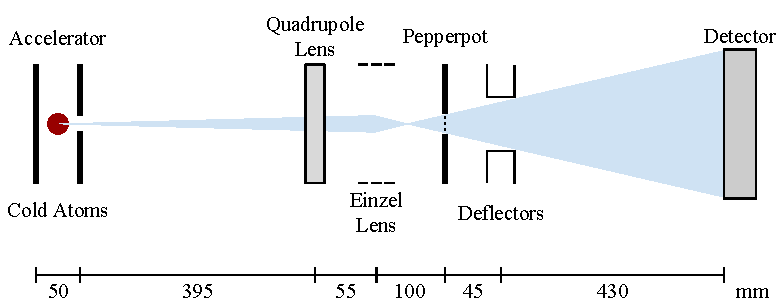
\includegraphics{part2/Figs/EmittanceApparatusSchematic.pdf}
\caption{A schematic of the experimental apparatus with relavent dimensions. The blue region indicates the electron beam envelope. Note that the deflectors would be orientated into and out of the page if depicted realistically.}
\label{figure:emittance_schematic}
\end{figure}

\subsection{Beam Optics}
The quadrupole electron optics discussed in Section \ref{section:quadrupole} were use to reduce the astigmatism present in the electron beam as discussed in the aforementioned section.
The two-dimensional pepperpot provide another avenue to monitor the astigmatism of the beam as with an astigmatic beam the spacing of the beamlets on the detector are not the same along each axis as shown in Figure~\ref{figure:astigmatic_pepperpot}.
When focussing was required the Einzel lens was used.

\begin{figure}
    \center
    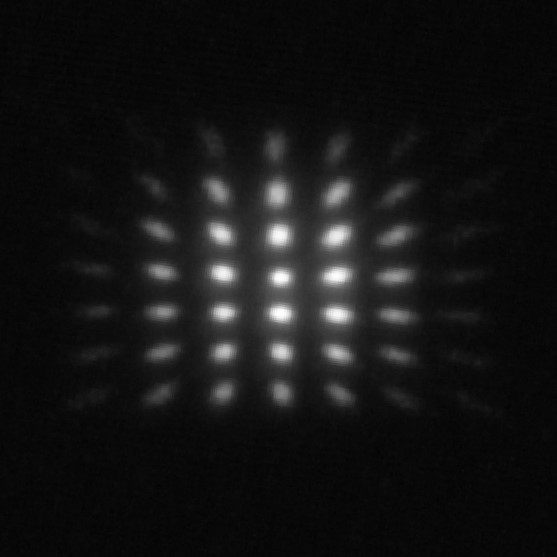
\includegraphics[width=0.5\linewidth]{part2/Figs/example_astigmatic_pepperpot.jpeg}
    \caption{An example of a pepperpot without the beam correction from the quadrupole lens. It is readily apparent that spacing of the beamlets is not the same for the $x$ and $y$ axes. This image is log scaled.}
    \label{figure:astigmatic_pepperpot}
\end{figure}

A number of permanent magnets were used to steer the beam through the various apertures and onto the detector and care was taken to attempt to keep the beam on the central axis of the apparatus.
This was achieved by manually adjusting the positions of the magnets, which were mounted on posts external to the vacuum system, to ensure that the beam was passing through the apertures in the system and by scanning the Einzel lens to verify that the beam was passing through its centre.
Due to the unstable nature of the apparatus these magnets needed to be adjusted on a day-to-day basis to maintain the beam path.

The main limiting factor to pepperpot emittance measurements using the \gls{caeis} was flux so the flux through the pepperpots was optimised by using the Einzel lens to focus the beam to the approximate size of the pepperpots at the pepperpot plane thus maximsing the flux through the apertures.
This required a Einzel lens voltage of \unit[4.8][kV].

\subsection{Beam Energy}
In many emittance measurements the beam energy would not be a free parameter however is this experiment we are able to vary the energy of our beam from a few hundred eV to around \unit[10]{keV}.
There are a number of considerations in determining the optimal beam energy to use for pepperpot measurements such as measurement resolution, beam current and beam stability.

The resolution of a pepperpot measurement is greater when the size of the beamlets on the detector is larger and, as shown in Equation~\ref{equation:divergence} the divergence is greater for slower beams.
Unfortunately the slower the beam the more fragile the alignment of the beam becomes.
While attempting to align a \unit[500][eV] beam through it system it was impossible to position the steering magnets such that an unobstructed beam made it through the system to the detector.

A relatively high energy beam of \unit[8]{keV} was used as this provided a robust beam alignment that was resistant to the transient changes in the magnetic environment.

\subsection{Bellows}

The bellows provide an additional mechanism to control the resolution of the measurement by adjusting the propagation distance of the pepperpot beamlets and thus their size on the detector.
As this parameter is also adjustable with the strength of the Einzel lens the bellows were placed approximately halfway between the minimumm and maximum position where the beam alignment was still well behaved.

\subsection{Streaking}
The streaking was performed using a pair of deflectors located after the pepperpot sample and orientated such that the one-dimensional pepperpots could be streaked across the detector.
For these measurements one deflector was grounded and the other given a time-varying voltage which was supplied in one of two ways:
\begin{itemize}
\item A fast ramp using a bipolar push-pull solid-state switch with a fixed transition time of \unit[10]{ns} and
\item A slower ramp using an amplified signal generator with a minimum transition of approximately \unit[10]{$\mu$s}.
\end{itemize}
An example of the voltage ramps is shown in Figure~\ref{figure:deflector_voltages}. The slow ramp was done by amplifying the output of signal generator\footnote{Rigol DG4162, able to operate up to \unit[160]{MHz}} which is highly configurable and thus cabable of a wide range of pulse lengths, limited by the speed of the amplifier to a transition time approximately \unit[10]{$\mu$s} in duration as shown in Figure~\ref{figure:deflector_voltages}.

Synchronisation with the experimental cycle was easily achieved using triggers from the pulse blaster {\color{red}(refer to description elsewhere?)} and, while the pulse blaster did not have sufficient temporal resolution to correctly trigger the fast ramp, adjusting cable lengths for the trigger signal by a couple of meters provided an adequate delay.

{\color{red}slow streaking smoothing of rigol signal, ringing in fast, calibrating the images}
\begin{figure}\label{figure:deflector_voltages}
    \center
    %% Creator: Matplotlib, PGF backend
%%
%% To include the figure in your LaTeX document, write
%%   \input{<filename>.pgf}
%%
%% Make sure the required packages are loaded in your preamble
%%   \usepackage{pgf}
%%
%% Figures using additional raster images can only be included by \input if
%% they are in the same directory as the main LaTeX file. For loading figures
%% from other directories you can use the `import` package
%%   \usepackage{import}
%% and then include the figures with
%%   \import{<path to file>}{<filename>.pgf}
%%
%% Matplotlib used the following preamble
%%
\begingroup%
\makeatletter%
\begin{pgfpicture}%
\pgfpathrectangle{\pgfpointorigin}{\pgfqpoint{5.710000in}{1.903333in}}%
\pgfusepath{use as bounding box, clip}%
\begin{pgfscope}%
\pgfsetbuttcap%
\pgfsetmiterjoin%
\definecolor{currentfill}{rgb}{1.000000,1.000000,1.000000}%
\pgfsetfillcolor{currentfill}%
\pgfsetlinewidth{0.000000pt}%
\definecolor{currentstroke}{rgb}{1.000000,1.000000,1.000000}%
\pgfsetstrokecolor{currentstroke}%
\pgfsetdash{}{0pt}%
\pgfpathmoveto{\pgfqpoint{0.000000in}{0.000000in}}%
\pgfpathlineto{\pgfqpoint{5.710000in}{0.000000in}}%
\pgfpathlineto{\pgfqpoint{5.710000in}{1.903333in}}%
\pgfpathlineto{\pgfqpoint{0.000000in}{1.903333in}}%
\pgfpathclose%
\pgfusepath{fill}%
\end{pgfscope}%
\begin{pgfscope}%
\pgfsetbuttcap%
\pgfsetmiterjoin%
\definecolor{currentfill}{rgb}{1.000000,1.000000,1.000000}%
\pgfsetfillcolor{currentfill}%
\pgfsetlinewidth{0.000000pt}%
\definecolor{currentstroke}{rgb}{0.000000,0.000000,0.000000}%
\pgfsetstrokecolor{currentstroke}%
\pgfsetstrokeopacity{0.000000}%
\pgfsetdash{}{0pt}%
\pgfpathmoveto{\pgfqpoint{0.661914in}{0.570703in}}%
\pgfpathlineto{\pgfqpoint{3.110957in}{0.570703in}}%
\pgfpathlineto{\pgfqpoint{3.110957in}{1.753333in}}%
\pgfpathlineto{\pgfqpoint{0.661914in}{1.753333in}}%
\pgfpathclose%
\pgfusepath{fill}%
\end{pgfscope}%
\begin{pgfscope}%
\pgfpathrectangle{\pgfqpoint{0.661914in}{0.570703in}}{\pgfqpoint{2.449043in}{1.182630in}} %
\pgfusepath{clip}%
\pgfsetrectcap%
\pgfsetroundjoin%
\pgfsetlinewidth{1.003750pt}%
\definecolor{currentstroke}{rgb}{0.309804,0.478431,0.682353}%
\pgfsetstrokecolor{currentstroke}%
\pgfsetdash{}{0pt}%
\pgfpathmoveto{\pgfqpoint{0.661914in}{0.639863in}}%
\pgfpathlineto{\pgfqpoint{0.685907in}{0.638678in}}%
\pgfpathlineto{\pgfqpoint{0.688437in}{0.638833in}}%
\pgfpathlineto{\pgfqpoint{0.691552in}{0.639256in}}%
\pgfpathlineto{\pgfqpoint{0.710846in}{0.640263in}}%
\pgfpathlineto{\pgfqpoint{0.712757in}{0.639892in}}%
\pgfpathlineto{\pgfqpoint{0.716371in}{0.638523in}}%
\pgfpathlineto{\pgfqpoint{0.720898in}{0.639289in}}%
\pgfpathlineto{\pgfqpoint{0.723118in}{0.639239in}}%
\pgfpathlineto{\pgfqpoint{0.725751in}{0.638742in}}%
\pgfpathlineto{\pgfqpoint{0.730157in}{0.640450in}}%
\pgfpathlineto{\pgfqpoint{0.733238in}{0.640418in}}%
\pgfpathlineto{\pgfqpoint{0.735820in}{0.640113in}}%
\pgfpathlineto{\pgfqpoint{0.741534in}{0.638183in}}%
\pgfpathlineto{\pgfqpoint{0.743806in}{0.638528in}}%
\pgfpathlineto{\pgfqpoint{0.747042in}{0.639045in}}%
\pgfpathlineto{\pgfqpoint{0.752498in}{0.639197in}}%
\pgfpathlineto{\pgfqpoint{0.756921in}{0.640379in}}%
\pgfpathlineto{\pgfqpoint{0.760088in}{0.639106in}}%
\pgfpathlineto{\pgfqpoint{0.764064in}{0.638800in}}%
\pgfpathlineto{\pgfqpoint{0.769313in}{0.639684in}}%
\pgfpathlineto{\pgfqpoint{0.783805in}{0.639351in}}%
\pgfpathlineto{\pgfqpoint{0.792015in}{0.641048in}}%
\pgfpathlineto{\pgfqpoint{0.796215in}{0.640030in}}%
\pgfpathlineto{\pgfqpoint{0.807867in}{0.639090in}}%
\pgfpathlineto{\pgfqpoint{0.810448in}{0.639002in}}%
\pgfpathlineto{\pgfqpoint{0.816782in}{0.640631in}}%
\pgfpathlineto{\pgfqpoint{0.819278in}{0.639510in}}%
\pgfpathlineto{\pgfqpoint{0.821636in}{0.639273in}}%
\pgfpathlineto{\pgfqpoint{0.824338in}{0.639420in}}%
\pgfpathlineto{\pgfqpoint{0.826989in}{0.638791in}}%
\pgfpathlineto{\pgfqpoint{0.830242in}{0.639425in}}%
\pgfpathlineto{\pgfqpoint{0.836420in}{0.639113in}}%
\pgfpathlineto{\pgfqpoint{0.840482in}{0.638745in}}%
\pgfpathlineto{\pgfqpoint{0.842806in}{0.639399in}}%
\pgfpathlineto{\pgfqpoint{0.845181in}{0.639797in}}%
\pgfpathlineto{\pgfqpoint{0.849123in}{0.639023in}}%
\pgfpathlineto{\pgfqpoint{0.852668in}{0.639534in}}%
\pgfpathlineto{\pgfqpoint{0.857264in}{0.639722in}}%
\pgfpathlineto{\pgfqpoint{0.862427in}{0.640019in}}%
\pgfpathlineto{\pgfqpoint{0.865886in}{0.639236in}}%
\pgfpathlineto{\pgfqpoint{0.871790in}{0.639947in}}%
\pgfpathlineto{\pgfqpoint{0.874303in}{0.639239in}}%
\pgfpathlineto{\pgfqpoint{0.878933in}{0.639722in}}%
\pgfpathlineto{\pgfqpoint{0.886024in}{0.640670in}}%
\pgfpathlineto{\pgfqpoint{0.900481in}{0.665955in}}%
\pgfpathlineto{\pgfqpoint{0.914991in}{0.692189in}}%
\pgfpathlineto{\pgfqpoint{0.984335in}{0.811283in}}%
\pgfpathlineto{\pgfqpoint{0.986934in}{0.815749in}}%
\pgfpathlineto{\pgfqpoint{0.995781in}{0.831818in}}%
\pgfpathlineto{\pgfqpoint{1.009602in}{0.855721in}}%
\pgfpathlineto{\pgfqpoint{1.013491in}{0.861243in}}%
\pgfpathlineto{\pgfqpoint{1.023181in}{0.875697in}}%
\pgfpathlineto{\pgfqpoint{1.031236in}{0.887602in}}%
\pgfpathlineto{\pgfqpoint{1.044506in}{0.905297in}}%
\pgfpathlineto{\pgfqpoint{1.051305in}{0.916597in}}%
\pgfpathlineto{\pgfqpoint{1.099256in}{0.993578in}}%
\pgfpathlineto{\pgfqpoint{1.105572in}{1.002734in}}%
\pgfpathlineto{\pgfqpoint{1.121028in}{1.028128in}}%
\pgfpathlineto{\pgfqpoint{1.134109in}{1.047792in}}%
\pgfpathlineto{\pgfqpoint{1.137121in}{1.053476in}}%
\pgfpathlineto{\pgfqpoint{1.139995in}{1.056965in}}%
\pgfpathlineto{\pgfqpoint{1.142990in}{1.060511in}}%
\pgfpathlineto{\pgfqpoint{1.160460in}{1.089288in}}%
\pgfpathlineto{\pgfqpoint{1.198376in}{1.148417in}}%
\pgfpathlineto{\pgfqpoint{1.201302in}{1.153386in}}%
\pgfpathlineto{\pgfqpoint{1.205037in}{1.159542in}}%
\pgfpathlineto{\pgfqpoint{1.213677in}{1.171255in}}%
\pgfpathlineto{\pgfqpoint{1.220269in}{1.181702in}}%
\pgfpathlineto{\pgfqpoint{1.225588in}{1.189842in}}%
\pgfpathlineto{\pgfqpoint{1.236190in}{1.205469in}}%
\pgfpathlineto{\pgfqpoint{1.272230in}{1.255450in}}%
\pgfpathlineto{\pgfqpoint{1.276172in}{1.260278in}}%
\pgfpathlineto{\pgfqpoint{1.284846in}{1.273493in}}%
\pgfpathlineto{\pgfqpoint{1.301077in}{1.296105in}}%
\pgfpathlineto{\pgfqpoint{1.308288in}{1.305361in}}%
\pgfpathlineto{\pgfqpoint{1.312540in}{1.311632in}}%
\pgfpathlineto{\pgfqpoint{1.318237in}{1.319983in}}%
\pgfpathlineto{\pgfqpoint{1.331334in}{1.337047in}}%
\pgfpathlineto{\pgfqpoint{1.340715in}{1.348001in}}%
\pgfpathlineto{\pgfqpoint{1.360336in}{1.368650in}}%
\pgfpathlineto{\pgfqpoint{1.367186in}{1.371538in}}%
\pgfpathlineto{\pgfqpoint{1.369974in}{1.371728in}}%
\pgfpathlineto{\pgfqpoint{1.378580in}{1.372520in}}%
\pgfpathlineto{\pgfqpoint{1.382383in}{1.373033in}}%
\pgfpathlineto{\pgfqpoint{1.385671in}{1.372624in}}%
\pgfpathlineto{\pgfqpoint{1.391798in}{1.369904in}}%
\pgfpathlineto{\pgfqpoint{1.398751in}{1.367030in}}%
\pgfpathlineto{\pgfqpoint{1.401936in}{1.366306in}}%
\pgfpathlineto{\pgfqpoint{1.405051in}{1.365280in}}%
\pgfpathlineto{\pgfqpoint{1.412916in}{1.361527in}}%
\pgfpathlineto{\pgfqpoint{1.414620in}{1.360642in}}%
\pgfpathlineto{\pgfqpoint{1.418803in}{1.357469in}}%
\pgfpathlineto{\pgfqpoint{1.422830in}{1.356282in}}%
\pgfpathlineto{\pgfqpoint{1.449215in}{1.342742in}}%
\pgfpathlineto{\pgfqpoint{1.451763in}{1.341815in}}%
\pgfpathlineto{\pgfqpoint{1.458768in}{1.337920in}}%
\pgfpathlineto{\pgfqpoint{1.463879in}{1.335066in}}%
\pgfpathlineto{\pgfqpoint{1.482278in}{1.323278in}}%
\pgfpathlineto{\pgfqpoint{1.486289in}{1.321369in}}%
\pgfpathlineto{\pgfqpoint{1.489301in}{1.319998in}}%
\pgfpathlineto{\pgfqpoint{1.491676in}{1.318482in}}%
\pgfpathlineto{\pgfqpoint{1.496702in}{1.315281in}}%
\pgfpathlineto{\pgfqpoint{1.508027in}{1.307857in}}%
\pgfpathlineto{\pgfqpoint{1.512519in}{1.305661in}}%
\pgfpathlineto{\pgfqpoint{1.536133in}{1.292034in}}%
\pgfpathlineto{\pgfqpoint{1.538680in}{1.290625in}}%
\pgfpathlineto{\pgfqpoint{1.543672in}{1.287161in}}%
\pgfpathlineto{\pgfqpoint{1.552604in}{1.281694in}}%
\pgfpathlineto{\pgfqpoint{1.559127in}{1.277377in}}%
\pgfpathlineto{\pgfqpoint{1.588060in}{1.259416in}}%
\pgfpathlineto{\pgfqpoint{1.592190in}{1.256355in}}%
\pgfpathlineto{\pgfqpoint{1.601450in}{1.251964in}}%
\pgfpathlineto{\pgfqpoint{1.606958in}{1.249291in}}%
\pgfpathlineto{\pgfqpoint{1.611054in}{1.245824in}}%
\pgfpathlineto{\pgfqpoint{1.616700in}{1.243599in}}%
\pgfpathlineto{\pgfqpoint{1.621983in}{1.241119in}}%
\pgfpathlineto{\pgfqpoint{1.624186in}{1.240234in}}%
\pgfpathlineto{\pgfqpoint{1.631312in}{1.234378in}}%
\pgfpathlineto{\pgfqpoint{1.650606in}{1.225090in}}%
\pgfpathlineto{\pgfqpoint{1.657542in}{1.220294in}}%
\pgfpathlineto{\pgfqpoint{1.663824in}{1.217270in}}%
\pgfpathlineto{\pgfqpoint{1.669280in}{1.214376in}}%
\pgfpathlineto{\pgfqpoint{1.671948in}{1.211721in}}%
\pgfpathlineto{\pgfqpoint{1.674513in}{1.209897in}}%
\pgfpathlineto{\pgfqpoint{1.677783in}{1.209593in}}%
\pgfpathlineto{\pgfqpoint{1.684977in}{1.206012in}}%
\pgfpathlineto{\pgfqpoint{1.687111in}{1.204250in}}%
\pgfpathlineto{\pgfqpoint{1.689986in}{1.202495in}}%
\pgfpathlineto{\pgfqpoint{1.693721in}{1.200464in}}%
\pgfpathlineto{\pgfqpoint{1.700622in}{1.196680in}}%
\pgfpathlineto{\pgfqpoint{1.702757in}{1.195139in}}%
\pgfpathlineto{\pgfqpoint{1.710261in}{1.189806in}}%
\pgfpathlineto{\pgfqpoint{1.712567in}{1.189085in}}%
\pgfpathlineto{\pgfqpoint{1.719090in}{1.184286in}}%
\pgfpathlineto{\pgfqpoint{1.722429in}{1.183228in}}%
\pgfpathlineto{\pgfqpoint{1.726250in}{1.179800in}}%
\pgfpathlineto{\pgfqpoint{1.731706in}{1.176591in}}%
\pgfpathlineto{\pgfqpoint{1.735596in}{1.174491in}}%
\pgfpathlineto{\pgfqpoint{1.738763in}{1.172988in}}%
\pgfpathlineto{\pgfqpoint{1.743479in}{1.169665in}}%
\pgfpathlineto{\pgfqpoint{1.746060in}{1.168250in}}%
\pgfpathlineto{\pgfqpoint{1.748418in}{1.166802in}}%
\pgfpathlineto{\pgfqpoint{1.760260in}{1.158948in}}%
\pgfpathlineto{\pgfqpoint{1.762928in}{1.158272in}}%
\pgfpathlineto{\pgfqpoint{1.767884in}{1.155173in}}%
\pgfpathlineto{\pgfqpoint{1.770673in}{1.153448in}}%
\pgfpathlineto{\pgfqpoint{1.774476in}{1.150514in}}%
\pgfpathlineto{\pgfqpoint{1.784614in}{1.143537in}}%
\pgfpathlineto{\pgfqpoint{1.794631in}{1.138029in}}%
\pgfpathlineto{\pgfqpoint{1.798831in}{1.135047in}}%
\pgfpathlineto{\pgfqpoint{1.806266in}{1.130913in}}%
\pgfpathlineto{\pgfqpoint{1.808090in}{1.130582in}}%
\pgfpathlineto{\pgfqpoint{1.815526in}{1.125060in}}%
\pgfpathlineto{\pgfqpoint{1.818658in}{1.123027in}}%
\pgfpathlineto{\pgfqpoint{1.827574in}{1.117849in}}%
\pgfpathlineto{\pgfqpoint{1.831567in}{1.115909in}}%
\pgfpathlineto{\pgfqpoint{1.835818in}{1.112834in}}%
\pgfpathlineto{\pgfqpoint{1.840706in}{1.110276in}}%
\pgfpathlineto{\pgfqpoint{1.850138in}{1.104195in}}%
\pgfpathlineto{\pgfqpoint{1.856368in}{1.100209in}}%
\pgfpathlineto{\pgfqpoint{1.859053in}{1.097177in}}%
\pgfpathlineto{\pgfqpoint{1.861463in}{1.095397in}}%
\pgfpathlineto{\pgfqpoint{1.864182in}{1.095064in}}%
\pgfpathlineto{\pgfqpoint{1.869724in}{1.091371in}}%
\pgfpathlineto{\pgfqpoint{1.872926in}{1.090020in}}%
\pgfpathlineto{\pgfqpoint{1.877831in}{1.086397in}}%
\pgfpathlineto{\pgfqpoint{1.881015in}{1.084090in}}%
\pgfpathlineto{\pgfqpoint{1.884681in}{1.081387in}}%
\pgfpathlineto{\pgfqpoint{1.898261in}{1.072633in}}%
\pgfpathlineto{\pgfqpoint{1.900963in}{1.070734in}}%
\pgfpathlineto{\pgfqpoint{1.904044in}{1.070255in}}%
\pgfpathlineto{\pgfqpoint{1.908605in}{1.067369in}}%
\pgfpathlineto{\pgfqpoint{1.920756in}{1.059650in}}%
\pgfpathlineto{\pgfqpoint{1.925610in}{1.057090in}}%
\pgfpathlineto{\pgfqpoint{1.935093in}{1.050792in}}%
\pgfpathlineto{\pgfqpoint{1.938759in}{1.048798in}}%
\pgfpathlineto{\pgfqpoint{1.943544in}{1.046823in}}%
\pgfpathlineto{\pgfqpoint{1.949465in}{1.041619in}}%
\pgfpathlineto{\pgfqpoint{1.952012in}{1.040593in}}%
\pgfpathlineto{\pgfqpoint{1.958484in}{1.036372in}}%
\pgfpathlineto{\pgfqpoint{1.961410in}{1.035261in}}%
\pgfpathlineto{\pgfqpoint{1.974748in}{1.026341in}}%
\pgfpathlineto{\pgfqpoint{1.978242in}{1.023999in}}%
\pgfpathlineto{\pgfqpoint{2.002252in}{1.010029in}}%
\pgfpathlineto{\pgfqpoint{2.004507in}{1.009139in}}%
\pgfpathlineto{\pgfqpoint{2.014610in}{1.001981in}}%
\pgfpathlineto{\pgfqpoint{2.019068in}{0.999305in}}%
\pgfpathlineto{\pgfqpoint{2.027037in}{0.994125in}}%
\pgfpathlineto{\pgfqpoint{2.029412in}{0.993518in}}%
\pgfpathlineto{\pgfqpoint{2.036107in}{0.988622in}}%
\pgfpathlineto{\pgfqpoint{2.038534in}{0.987743in}}%
\pgfpathlineto{\pgfqpoint{2.046417in}{0.980597in}}%
\pgfpathlineto{\pgfqpoint{2.067569in}{0.969592in}}%
\pgfpathlineto{\pgfqpoint{2.082182in}{0.960328in}}%
\pgfpathlineto{\pgfqpoint{2.085314in}{0.958055in}}%
\pgfpathlineto{\pgfqpoint{2.088481in}{0.955629in}}%
\pgfpathlineto{\pgfqpoint{2.091545in}{0.954590in}}%
\pgfpathlineto{\pgfqpoint{2.095211in}{0.953371in}}%
\pgfpathlineto{\pgfqpoint{2.113335in}{0.941803in}}%
\pgfpathlineto{\pgfqpoint{2.119014in}{0.938511in}}%
\pgfpathlineto{\pgfqpoint{2.122095in}{0.936371in}}%
\pgfpathlineto{\pgfqpoint{2.128136in}{0.932720in}}%
\pgfpathlineto{\pgfqpoint{2.133868in}{0.928294in}}%
\pgfpathlineto{\pgfqpoint{2.140391in}{0.925112in}}%
\pgfpathlineto{\pgfqpoint{2.146621in}{0.922096in}}%
\pgfpathlineto{\pgfqpoint{2.153506in}{0.918316in}}%
\pgfpathlineto{\pgfqpoint{2.157757in}{0.915177in}}%
\pgfpathlineto{\pgfqpoint{2.168359in}{0.909577in}}%
\pgfpathlineto{\pgfqpoint{2.172473in}{0.908267in}}%
\pgfpathlineto{\pgfqpoint{2.179444in}{0.904189in}}%
\pgfpathlineto{\pgfqpoint{2.195347in}{0.897681in}}%
\pgfpathlineto{\pgfqpoint{2.201440in}{0.894094in}}%
\pgfpathlineto{\pgfqpoint{2.206638in}{0.891776in}}%
\pgfpathlineto{\pgfqpoint{2.210906in}{0.888936in}}%
\pgfpathlineto{\pgfqpoint{2.238324in}{0.876719in}}%
\pgfpathlineto{\pgfqpoint{2.249701in}{0.870489in}}%
\pgfpathlineto{\pgfqpoint{2.255415in}{0.868058in}}%
\pgfpathlineto{\pgfqpoint{2.259477in}{0.865983in}}%
\pgfpathlineto{\pgfqpoint{2.296189in}{0.846240in}}%
\pgfpathlineto{\pgfqpoint{2.298529in}{0.845255in}}%
\pgfpathlineto{\pgfqpoint{2.330302in}{0.826656in}}%
\pgfpathlineto{\pgfqpoint{2.333141in}{0.826143in}}%
\pgfpathlineto{\pgfqpoint{2.339217in}{0.823781in}}%
\pgfpathlineto{\pgfqpoint{2.345310in}{0.819608in}}%
\pgfpathlineto{\pgfqpoint{2.352504in}{0.815799in}}%
\pgfpathlineto{\pgfqpoint{2.356153in}{0.814386in}}%
\pgfpathlineto{\pgfqpoint{2.370507in}{0.806952in}}%
\pgfpathlineto{\pgfqpoint{2.372263in}{0.806205in}}%
\pgfpathlineto{\pgfqpoint{2.375757in}{0.803834in}}%
\pgfpathlineto{\pgfqpoint{2.379027in}{0.802493in}}%
\pgfpathlineto{\pgfqpoint{2.384535in}{0.798330in}}%
\pgfpathlineto{\pgfqpoint{2.387254in}{0.796928in}}%
\pgfpathlineto{\pgfqpoint{2.390559in}{0.796050in}}%
\pgfpathlineto{\pgfqpoint{2.414810in}{0.784334in}}%
\pgfpathlineto{\pgfqpoint{2.418785in}{0.782833in}}%
\pgfpathlineto{\pgfqpoint{2.424362in}{0.780593in}}%
\pgfpathlineto{\pgfqpoint{2.426272in}{0.779517in}}%
\pgfpathlineto{\pgfqpoint{2.429456in}{0.777818in}}%
\pgfpathlineto{\pgfqpoint{2.435859in}{0.774243in}}%
\pgfpathlineto{\pgfqpoint{2.443329in}{0.770718in}}%
\pgfpathlineto{\pgfqpoint{2.446100in}{0.768410in}}%
\pgfpathlineto{\pgfqpoint{2.450592in}{0.765258in}}%
\pgfpathlineto{\pgfqpoint{2.459594in}{0.761596in}}%
\pgfpathlineto{\pgfqpoint{2.464464in}{0.758944in}}%
\pgfpathlineto{\pgfqpoint{2.470781in}{0.755581in}}%
\pgfpathlineto{\pgfqpoint{2.473914in}{0.754105in}}%
\pgfpathlineto{\pgfqpoint{2.482571in}{0.751605in}}%
\pgfpathlineto{\pgfqpoint{2.491762in}{0.746004in}}%
\pgfpathlineto{\pgfqpoint{2.495548in}{0.744999in}}%
\pgfpathlineto{\pgfqpoint{2.501779in}{0.741339in}}%
\pgfpathlineto{\pgfqpoint{2.506391in}{0.738890in}}%
\pgfpathlineto{\pgfqpoint{2.512880in}{0.736913in}}%
\pgfpathlineto{\pgfqpoint{2.515135in}{0.735100in}}%
\pgfpathlineto{\pgfqpoint{2.518164in}{0.733531in}}%
\pgfpathlineto{\pgfqpoint{2.521658in}{0.733234in}}%
\pgfpathlineto{\pgfqpoint{2.534584in}{0.726799in}}%
\pgfpathlineto{\pgfqpoint{2.538198in}{0.725167in}}%
\pgfpathlineto{\pgfqpoint{2.540694in}{0.724174in}}%
\pgfpathlineto{\pgfqpoint{2.543809in}{0.723993in}}%
\pgfpathlineto{\pgfqpoint{2.549953in}{0.720387in}}%
\pgfpathlineto{\pgfqpoint{2.553860in}{0.718642in}}%
\pgfpathlineto{\pgfqpoint{2.577423in}{0.707790in}}%
\pgfpathlineto{\pgfqpoint{2.582793in}{0.704677in}}%
\pgfpathlineto{\pgfqpoint{2.590710in}{0.702237in}}%
\pgfpathlineto{\pgfqpoint{2.601226in}{0.697290in}}%
\pgfpathlineto{\pgfqpoint{2.603774in}{0.696608in}}%
\pgfpathlineto{\pgfqpoint{2.606699in}{0.695425in}}%
\pgfpathlineto{\pgfqpoint{2.612104in}{0.692573in}}%
\pgfpathlineto{\pgfqpoint{2.615150in}{0.691304in}}%
\pgfpathlineto{\pgfqpoint{2.618730in}{0.691350in}}%
\pgfpathlineto{\pgfqpoint{2.620899in}{0.690780in}}%
\pgfpathlineto{\pgfqpoint{2.626148in}{0.687996in}}%
\pgfpathlineto{\pgfqpoint{2.629212in}{0.686733in}}%
\pgfpathlineto{\pgfqpoint{2.636578in}{0.681893in}}%
\pgfpathlineto{\pgfqpoint{2.642207in}{0.679494in}}%
\pgfpathlineto{\pgfqpoint{2.645064in}{0.677502in}}%
\pgfpathlineto{\pgfqpoint{2.649194in}{0.676921in}}%
\pgfpathlineto{\pgfqpoint{2.655304in}{0.674018in}}%
\pgfpathlineto{\pgfqpoint{2.658265in}{0.673861in}}%
\pgfpathlineto{\pgfqpoint{2.660451in}{0.672657in}}%
\pgfpathlineto{\pgfqpoint{2.664220in}{0.669872in}}%
\pgfpathlineto{\pgfqpoint{2.668179in}{0.668853in}}%
\pgfpathlineto{\pgfqpoint{2.672808in}{0.667316in}}%
\pgfpathlineto{\pgfqpoint{2.676802in}{0.665872in}}%
\pgfpathlineto{\pgfqpoint{2.681913in}{0.662074in}}%
\pgfpathlineto{\pgfqpoint{2.685820in}{0.660915in}}%
\pgfpathlineto{\pgfqpoint{2.690708in}{0.659040in}}%
\pgfpathlineto{\pgfqpoint{2.697404in}{0.657197in}}%
\pgfpathlineto{\pgfqpoint{2.700467in}{0.656157in}}%
\pgfpathlineto{\pgfqpoint{2.705992in}{0.654526in}}%
\pgfpathlineto{\pgfqpoint{2.710484in}{0.651805in}}%
\pgfpathlineto{\pgfqpoint{2.736473in}{0.644770in}}%
\pgfpathlineto{\pgfqpoint{2.740243in}{0.645682in}}%
\pgfpathlineto{\pgfqpoint{2.743840in}{0.644184in}}%
\pgfpathlineto{\pgfqpoint{2.746680in}{0.644043in}}%
\pgfpathlineto{\pgfqpoint{2.755389in}{0.644388in}}%
\pgfpathlineto{\pgfqpoint{2.758659in}{0.643327in}}%
\pgfpathlineto{\pgfqpoint{2.770862in}{0.643618in}}%
\pgfpathlineto{\pgfqpoint{2.773719in}{0.642939in}}%
\pgfpathlineto{\pgfqpoint{2.778091in}{0.642912in}}%
\pgfpathlineto{\pgfqpoint{2.781843in}{0.642376in}}%
\pgfpathlineto{\pgfqpoint{2.784545in}{0.642387in}}%
\pgfpathlineto{\pgfqpoint{2.793409in}{0.642164in}}%
\pgfpathlineto{\pgfqpoint{2.796197in}{0.642466in}}%
\pgfpathlineto{\pgfqpoint{2.830792in}{0.641798in}}%
\pgfpathlineto{\pgfqpoint{2.833924in}{0.641463in}}%
\pgfpathlineto{\pgfqpoint{2.836730in}{0.641891in}}%
\pgfpathlineto{\pgfqpoint{2.840706in}{0.641645in}}%
\pgfpathlineto{\pgfqpoint{2.847625in}{0.641870in}}%
\pgfpathlineto{\pgfqpoint{2.850327in}{0.641873in}}%
\pgfpathlineto{\pgfqpoint{2.854372in}{0.641692in}}%
\pgfpathlineto{\pgfqpoint{2.864578in}{0.640003in}}%
\pgfpathlineto{\pgfqpoint{2.867383in}{0.640282in}}%
\pgfpathlineto{\pgfqpoint{2.870912in}{0.640868in}}%
\pgfpathlineto{\pgfqpoint{2.874440in}{0.640202in}}%
\pgfpathlineto{\pgfqpoint{2.879173in}{0.641049in}}%
\pgfpathlineto{\pgfqpoint{2.882994in}{0.641235in}}%
\pgfpathlineto{\pgfqpoint{2.886591in}{0.641424in}}%
\pgfpathlineto{\pgfqpoint{2.891135in}{0.640226in}}%
\pgfpathlineto{\pgfqpoint{2.898588in}{0.640885in}}%
\pgfpathlineto{\pgfqpoint{2.903699in}{0.641801in}}%
\pgfpathlineto{\pgfqpoint{2.906952in}{0.641286in}}%
\pgfpathlineto{\pgfqpoint{2.911840in}{0.640658in}}%
\pgfpathlineto{\pgfqpoint{2.914904in}{0.640875in}}%
\pgfpathlineto{\pgfqpoint{2.921565in}{0.640269in}}%
\pgfpathlineto{\pgfqpoint{2.947244in}{0.639764in}}%
\pgfpathlineto{\pgfqpoint{2.950790in}{0.639702in}}%
\pgfpathlineto{\pgfqpoint{2.954508in}{0.639759in}}%
\pgfpathlineto{\pgfqpoint{2.957571in}{0.640221in}}%
\pgfpathlineto{\pgfqpoint{2.961082in}{0.640886in}}%
\pgfpathlineto{\pgfqpoint{2.964370in}{0.641031in}}%
\pgfpathlineto{\pgfqpoint{2.968500in}{0.641910in}}%
\pgfpathlineto{\pgfqpoint{2.976555in}{0.640036in}}%
\pgfpathlineto{\pgfqpoint{2.983578in}{0.640519in}}%
\pgfpathlineto{\pgfqpoint{2.986004in}{0.640597in}}%
\pgfpathlineto{\pgfqpoint{2.992614in}{0.641391in}}%
\pgfpathlineto{\pgfqpoint{2.996555in}{0.639939in}}%
\pgfpathlineto{\pgfqpoint{3.001168in}{0.640445in}}%
\pgfpathlineto{\pgfqpoint{3.004816in}{0.640508in}}%
\pgfpathlineto{\pgfqpoint{3.010290in}{0.639787in}}%
\pgfpathlineto{\pgfqpoint{3.013353in}{0.638891in}}%
\pgfpathlineto{\pgfqpoint{3.017725in}{0.639497in}}%
\pgfpathlineto{\pgfqpoint{3.027088in}{0.640419in}}%
\pgfpathlineto{\pgfqpoint{3.031116in}{0.639390in}}%
\pgfpathlineto{\pgfqpoint{3.034041in}{0.639799in}}%
\pgfpathlineto{\pgfqpoint{3.036417in}{0.639462in}}%
\pgfpathlineto{\pgfqpoint{3.039377in}{0.638991in}}%
\pgfpathlineto{\pgfqpoint{3.044489in}{0.638961in}}%
\pgfpathlineto{\pgfqpoint{3.046812in}{0.638655in}}%
\pgfpathlineto{\pgfqpoint{3.052096in}{0.639880in}}%
\pgfpathlineto{\pgfqpoint{3.058671in}{0.639665in}}%
\pgfpathlineto{\pgfqpoint{3.062389in}{0.638985in}}%
\pgfpathlineto{\pgfqpoint{3.065022in}{0.638876in}}%
\pgfpathlineto{\pgfqpoint{3.067879in}{0.638195in}}%
\pgfpathlineto{\pgfqpoint{3.071339in}{0.639036in}}%
\pgfpathlineto{\pgfqpoint{3.076829in}{0.639563in}}%
\pgfpathlineto{\pgfqpoint{3.080048in}{0.639522in}}%
\pgfpathlineto{\pgfqpoint{3.084299in}{0.639254in}}%
\pgfpathlineto{\pgfqpoint{3.110959in}{0.639799in}}%
\pgfpathlineto{\pgfqpoint{3.110959in}{0.639799in}}%
\pgfusepath{stroke}%
\end{pgfscope}%
\begin{pgfscope}%
\pgfpathrectangle{\pgfqpoint{0.661914in}{0.570703in}}{\pgfqpoint{2.449043in}{1.182630in}} %
\pgfusepath{clip}%
\pgfsetbuttcap%
\pgfsetroundjoin%
\pgfsetlinewidth{1.003750pt}%
\definecolor{currentstroke}{rgb}{0.000000,0.000000,0.000000}%
\pgfsetstrokecolor{currentstroke}%
\pgfsetdash{{1.000000pt}{3.000000pt}}{0.000000pt}%
\pgfpathmoveto{\pgfqpoint{1.475874in}{0.570703in}}%
\pgfpathlineto{\pgfqpoint{1.475874in}{1.753333in}}%
\pgfusepath{stroke}%
\end{pgfscope}%
\begin{pgfscope}%
\pgfsetrectcap%
\pgfsetmiterjoin%
\pgfsetlinewidth{1.003750pt}%
\definecolor{currentstroke}{rgb}{0.000000,0.000000,0.000000}%
\pgfsetstrokecolor{currentstroke}%
\pgfsetdash{}{0pt}%
\pgfpathmoveto{\pgfqpoint{0.661914in}{0.570703in}}%
\pgfpathlineto{\pgfqpoint{3.110957in}{0.570703in}}%
\pgfusepath{stroke}%
\end{pgfscope}%
\begin{pgfscope}%
\pgfsetrectcap%
\pgfsetmiterjoin%
\pgfsetlinewidth{1.003750pt}%
\definecolor{currentstroke}{rgb}{0.000000,0.000000,0.000000}%
\pgfsetstrokecolor{currentstroke}%
\pgfsetdash{}{0pt}%
\pgfpathmoveto{\pgfqpoint{3.110957in}{0.570703in}}%
\pgfpathlineto{\pgfqpoint{3.110957in}{1.753333in}}%
\pgfusepath{stroke}%
\end{pgfscope}%
\begin{pgfscope}%
\pgfsetrectcap%
\pgfsetmiterjoin%
\pgfsetlinewidth{1.003750pt}%
\definecolor{currentstroke}{rgb}{0.000000,0.000000,0.000000}%
\pgfsetstrokecolor{currentstroke}%
\pgfsetdash{}{0pt}%
\pgfpathmoveto{\pgfqpoint{0.661914in}{1.753333in}}%
\pgfpathlineto{\pgfqpoint{3.110957in}{1.753333in}}%
\pgfusepath{stroke}%
\end{pgfscope}%
\begin{pgfscope}%
\pgfsetrectcap%
\pgfsetmiterjoin%
\pgfsetlinewidth{1.003750pt}%
\definecolor{currentstroke}{rgb}{0.000000,0.000000,0.000000}%
\pgfsetstrokecolor{currentstroke}%
\pgfsetdash{}{0pt}%
\pgfpathmoveto{\pgfqpoint{0.661914in}{0.570703in}}%
\pgfpathlineto{\pgfqpoint{0.661914in}{1.753333in}}%
\pgfusepath{stroke}%
\end{pgfscope}%
\begin{pgfscope}%
\pgfsetbuttcap%
\pgfsetroundjoin%
\definecolor{currentfill}{rgb}{0.000000,0.000000,0.000000}%
\pgfsetfillcolor{currentfill}%
\pgfsetlinewidth{0.501875pt}%
\definecolor{currentstroke}{rgb}{0.000000,0.000000,0.000000}%
\pgfsetstrokecolor{currentstroke}%
\pgfsetdash{}{0pt}%
\pgfsys@defobject{currentmarker}{\pgfqpoint{0.000000in}{0.000000in}}{\pgfqpoint{0.000000in}{0.055556in}}{%
\pgfpathmoveto{\pgfqpoint{0.000000in}{0.000000in}}%
\pgfpathlineto{\pgfqpoint{0.000000in}{0.055556in}}%
\pgfusepath{stroke,fill}%
}%
\begin{pgfscope}%
\pgfsys@transformshift{1.045589in}{0.570703in}%
\pgfsys@useobject{currentmarker}{}%
\end{pgfscope}%
\end{pgfscope}%
\begin{pgfscope}%
\pgfsetbuttcap%
\pgfsetroundjoin%
\definecolor{currentfill}{rgb}{0.000000,0.000000,0.000000}%
\pgfsetfillcolor{currentfill}%
\pgfsetlinewidth{0.501875pt}%
\definecolor{currentstroke}{rgb}{0.000000,0.000000,0.000000}%
\pgfsetstrokecolor{currentstroke}%
\pgfsetdash{}{0pt}%
\pgfsys@defobject{currentmarker}{\pgfqpoint{0.000000in}{-0.055556in}}{\pgfqpoint{0.000000in}{0.000000in}}{%
\pgfpathmoveto{\pgfqpoint{0.000000in}{0.000000in}}%
\pgfpathlineto{\pgfqpoint{0.000000in}{-0.055556in}}%
\pgfusepath{stroke,fill}%
}%
\begin{pgfscope}%
\pgfsys@transformshift{1.045589in}{1.753333in}%
\pgfsys@useobject{currentmarker}{}%
\end{pgfscope}%
\end{pgfscope}%
\begin{pgfscope}%
\pgftext[x=1.045589in,y=0.515148in,,top]{\fontsize{10.000000}{12.000000}\selectfont -5}%
\end{pgfscope}%
\begin{pgfscope}%
\pgfsetbuttcap%
\pgfsetroundjoin%
\definecolor{currentfill}{rgb}{0.000000,0.000000,0.000000}%
\pgfsetfillcolor{currentfill}%
\pgfsetlinewidth{0.501875pt}%
\definecolor{currentstroke}{rgb}{0.000000,0.000000,0.000000}%
\pgfsetstrokecolor{currentstroke}%
\pgfsetdash{}{0pt}%
\pgfsys@defobject{currentmarker}{\pgfqpoint{0.000000in}{0.000000in}}{\pgfqpoint{0.000000in}{0.055556in}}{%
\pgfpathmoveto{\pgfqpoint{0.000000in}{0.000000in}}%
\pgfpathlineto{\pgfqpoint{0.000000in}{0.055556in}}%
\pgfusepath{stroke,fill}%
}%
\begin{pgfscope}%
\pgfsys@transformshift{1.475874in}{0.570703in}%
\pgfsys@useobject{currentmarker}{}%
\end{pgfscope}%
\end{pgfscope}%
\begin{pgfscope}%
\pgfsetbuttcap%
\pgfsetroundjoin%
\definecolor{currentfill}{rgb}{0.000000,0.000000,0.000000}%
\pgfsetfillcolor{currentfill}%
\pgfsetlinewidth{0.501875pt}%
\definecolor{currentstroke}{rgb}{0.000000,0.000000,0.000000}%
\pgfsetstrokecolor{currentstroke}%
\pgfsetdash{}{0pt}%
\pgfsys@defobject{currentmarker}{\pgfqpoint{0.000000in}{-0.055556in}}{\pgfqpoint{0.000000in}{0.000000in}}{%
\pgfpathmoveto{\pgfqpoint{0.000000in}{0.000000in}}%
\pgfpathlineto{\pgfqpoint{0.000000in}{-0.055556in}}%
\pgfusepath{stroke,fill}%
}%
\begin{pgfscope}%
\pgfsys@transformshift{1.475874in}{1.753333in}%
\pgfsys@useobject{currentmarker}{}%
\end{pgfscope}%
\end{pgfscope}%
\begin{pgfscope}%
\pgftext[x=1.475874in,y=0.515148in,,top]{\fontsize{10.000000}{12.000000}\selectfont 0}%
\end{pgfscope}%
\begin{pgfscope}%
\pgfsetbuttcap%
\pgfsetroundjoin%
\definecolor{currentfill}{rgb}{0.000000,0.000000,0.000000}%
\pgfsetfillcolor{currentfill}%
\pgfsetlinewidth{0.501875pt}%
\definecolor{currentstroke}{rgb}{0.000000,0.000000,0.000000}%
\pgfsetstrokecolor{currentstroke}%
\pgfsetdash{}{0pt}%
\pgfsys@defobject{currentmarker}{\pgfqpoint{0.000000in}{0.000000in}}{\pgfqpoint{0.000000in}{0.055556in}}{%
\pgfpathmoveto{\pgfqpoint{0.000000in}{0.000000in}}%
\pgfpathlineto{\pgfqpoint{0.000000in}{0.055556in}}%
\pgfusepath{stroke,fill}%
}%
\begin{pgfscope}%
\pgfsys@transformshift{1.906159in}{0.570703in}%
\pgfsys@useobject{currentmarker}{}%
\end{pgfscope}%
\end{pgfscope}%
\begin{pgfscope}%
\pgfsetbuttcap%
\pgfsetroundjoin%
\definecolor{currentfill}{rgb}{0.000000,0.000000,0.000000}%
\pgfsetfillcolor{currentfill}%
\pgfsetlinewidth{0.501875pt}%
\definecolor{currentstroke}{rgb}{0.000000,0.000000,0.000000}%
\pgfsetstrokecolor{currentstroke}%
\pgfsetdash{}{0pt}%
\pgfsys@defobject{currentmarker}{\pgfqpoint{0.000000in}{-0.055556in}}{\pgfqpoint{0.000000in}{0.000000in}}{%
\pgfpathmoveto{\pgfqpoint{0.000000in}{0.000000in}}%
\pgfpathlineto{\pgfqpoint{0.000000in}{-0.055556in}}%
\pgfusepath{stroke,fill}%
}%
\begin{pgfscope}%
\pgfsys@transformshift{1.906159in}{1.753333in}%
\pgfsys@useobject{currentmarker}{}%
\end{pgfscope}%
\end{pgfscope}%
\begin{pgfscope}%
\pgftext[x=1.906159in,y=0.515148in,,top]{\fontsize{10.000000}{12.000000}\selectfont 5}%
\end{pgfscope}%
\begin{pgfscope}%
\pgfsetbuttcap%
\pgfsetroundjoin%
\definecolor{currentfill}{rgb}{0.000000,0.000000,0.000000}%
\pgfsetfillcolor{currentfill}%
\pgfsetlinewidth{0.501875pt}%
\definecolor{currentstroke}{rgb}{0.000000,0.000000,0.000000}%
\pgfsetstrokecolor{currentstroke}%
\pgfsetdash{}{0pt}%
\pgfsys@defobject{currentmarker}{\pgfqpoint{0.000000in}{0.000000in}}{\pgfqpoint{0.000000in}{0.055556in}}{%
\pgfpathmoveto{\pgfqpoint{0.000000in}{0.000000in}}%
\pgfpathlineto{\pgfqpoint{0.000000in}{0.055556in}}%
\pgfusepath{stroke,fill}%
}%
\begin{pgfscope}%
\pgfsys@transformshift{2.336444in}{0.570703in}%
\pgfsys@useobject{currentmarker}{}%
\end{pgfscope}%
\end{pgfscope}%
\begin{pgfscope}%
\pgfsetbuttcap%
\pgfsetroundjoin%
\definecolor{currentfill}{rgb}{0.000000,0.000000,0.000000}%
\pgfsetfillcolor{currentfill}%
\pgfsetlinewidth{0.501875pt}%
\definecolor{currentstroke}{rgb}{0.000000,0.000000,0.000000}%
\pgfsetstrokecolor{currentstroke}%
\pgfsetdash{}{0pt}%
\pgfsys@defobject{currentmarker}{\pgfqpoint{0.000000in}{-0.055556in}}{\pgfqpoint{0.000000in}{0.000000in}}{%
\pgfpathmoveto{\pgfqpoint{0.000000in}{0.000000in}}%
\pgfpathlineto{\pgfqpoint{0.000000in}{-0.055556in}}%
\pgfusepath{stroke,fill}%
}%
\begin{pgfscope}%
\pgfsys@transformshift{2.336444in}{1.753333in}%
\pgfsys@useobject{currentmarker}{}%
\end{pgfscope}%
\end{pgfscope}%
\begin{pgfscope}%
\pgftext[x=2.336444in,y=0.515148in,,top]{\fontsize{10.000000}{12.000000}\selectfont 10}%
\end{pgfscope}%
\begin{pgfscope}%
\pgfsetbuttcap%
\pgfsetroundjoin%
\definecolor{currentfill}{rgb}{0.000000,0.000000,0.000000}%
\pgfsetfillcolor{currentfill}%
\pgfsetlinewidth{0.501875pt}%
\definecolor{currentstroke}{rgb}{0.000000,0.000000,0.000000}%
\pgfsetstrokecolor{currentstroke}%
\pgfsetdash{}{0pt}%
\pgfsys@defobject{currentmarker}{\pgfqpoint{0.000000in}{0.000000in}}{\pgfqpoint{0.000000in}{0.055556in}}{%
\pgfpathmoveto{\pgfqpoint{0.000000in}{0.000000in}}%
\pgfpathlineto{\pgfqpoint{0.000000in}{0.055556in}}%
\pgfusepath{stroke,fill}%
}%
\begin{pgfscope}%
\pgfsys@transformshift{2.766729in}{0.570703in}%
\pgfsys@useobject{currentmarker}{}%
\end{pgfscope}%
\end{pgfscope}%
\begin{pgfscope}%
\pgfsetbuttcap%
\pgfsetroundjoin%
\definecolor{currentfill}{rgb}{0.000000,0.000000,0.000000}%
\pgfsetfillcolor{currentfill}%
\pgfsetlinewidth{0.501875pt}%
\definecolor{currentstroke}{rgb}{0.000000,0.000000,0.000000}%
\pgfsetstrokecolor{currentstroke}%
\pgfsetdash{}{0pt}%
\pgfsys@defobject{currentmarker}{\pgfqpoint{0.000000in}{-0.055556in}}{\pgfqpoint{0.000000in}{0.000000in}}{%
\pgfpathmoveto{\pgfqpoint{0.000000in}{0.000000in}}%
\pgfpathlineto{\pgfqpoint{0.000000in}{-0.055556in}}%
\pgfusepath{stroke,fill}%
}%
\begin{pgfscope}%
\pgfsys@transformshift{2.766729in}{1.753333in}%
\pgfsys@useobject{currentmarker}{}%
\end{pgfscope}%
\end{pgfscope}%
\begin{pgfscope}%
\pgftext[x=2.766729in,y=0.515148in,,top]{\fontsize{10.000000}{12.000000}\selectfont 15}%
\end{pgfscope}%
\begin{pgfscope}%
\pgftext[x=1.886436in,y=0.322246in,,top]{\fontsize{10.000000}{12.000000}\selectfont Time (\(\displaystyle \muup\)s)}%
\end{pgfscope}%
\begin{pgfscope}%
\pgfsetbuttcap%
\pgfsetroundjoin%
\definecolor{currentfill}{rgb}{0.000000,0.000000,0.000000}%
\pgfsetfillcolor{currentfill}%
\pgfsetlinewidth{0.501875pt}%
\definecolor{currentstroke}{rgb}{0.000000,0.000000,0.000000}%
\pgfsetstrokecolor{currentstroke}%
\pgfsetdash{}{0pt}%
\pgfsys@defobject{currentmarker}{\pgfqpoint{0.000000in}{0.000000in}}{\pgfqpoint{0.055556in}{0.000000in}}{%
\pgfpathmoveto{\pgfqpoint{0.000000in}{0.000000in}}%
\pgfpathlineto{\pgfqpoint{0.055556in}{0.000000in}}%
\pgfusepath{stroke,fill}%
}%
\begin{pgfscope}%
\pgfsys@transformshift{0.661914in}{0.636405in}%
\pgfsys@useobject{currentmarker}{}%
\end{pgfscope}%
\end{pgfscope}%
\begin{pgfscope}%
\pgfsetbuttcap%
\pgfsetroundjoin%
\definecolor{currentfill}{rgb}{0.000000,0.000000,0.000000}%
\pgfsetfillcolor{currentfill}%
\pgfsetlinewidth{0.501875pt}%
\definecolor{currentstroke}{rgb}{0.000000,0.000000,0.000000}%
\pgfsetstrokecolor{currentstroke}%
\pgfsetdash{}{0pt}%
\pgfsys@defobject{currentmarker}{\pgfqpoint{-0.055556in}{0.000000in}}{\pgfqpoint{0.000000in}{0.000000in}}{%
\pgfpathmoveto{\pgfqpoint{0.000000in}{0.000000in}}%
\pgfpathlineto{\pgfqpoint{-0.055556in}{0.000000in}}%
\pgfusepath{stroke,fill}%
}%
\begin{pgfscope}%
\pgfsys@transformshift{3.110957in}{0.636405in}%
\pgfsys@useobject{currentmarker}{}%
\end{pgfscope}%
\end{pgfscope}%
\begin{pgfscope}%
\pgftext[x=0.606359in,y=0.636405in,right,]{\fontsize{10.000000}{12.000000}\selectfont -100}%
\end{pgfscope}%
\begin{pgfscope}%
\pgfsetbuttcap%
\pgfsetroundjoin%
\definecolor{currentfill}{rgb}{0.000000,0.000000,0.000000}%
\pgfsetfillcolor{currentfill}%
\pgfsetlinewidth{0.501875pt}%
\definecolor{currentstroke}{rgb}{0.000000,0.000000,0.000000}%
\pgfsetstrokecolor{currentstroke}%
\pgfsetdash{}{0pt}%
\pgfsys@defobject{currentmarker}{\pgfqpoint{0.000000in}{0.000000in}}{\pgfqpoint{0.055556in}{0.000000in}}{%
\pgfpathmoveto{\pgfqpoint{0.000000in}{0.000000in}}%
\pgfpathlineto{\pgfqpoint{0.055556in}{0.000000in}}%
\pgfusepath{stroke,fill}%
}%
\begin{pgfscope}%
\pgfsys@transformshift{0.661914in}{0.899212in}%
\pgfsys@useobject{currentmarker}{}%
\end{pgfscope}%
\end{pgfscope}%
\begin{pgfscope}%
\pgfsetbuttcap%
\pgfsetroundjoin%
\definecolor{currentfill}{rgb}{0.000000,0.000000,0.000000}%
\pgfsetfillcolor{currentfill}%
\pgfsetlinewidth{0.501875pt}%
\definecolor{currentstroke}{rgb}{0.000000,0.000000,0.000000}%
\pgfsetstrokecolor{currentstroke}%
\pgfsetdash{}{0pt}%
\pgfsys@defobject{currentmarker}{\pgfqpoint{-0.055556in}{0.000000in}}{\pgfqpoint{0.000000in}{0.000000in}}{%
\pgfpathmoveto{\pgfqpoint{0.000000in}{0.000000in}}%
\pgfpathlineto{\pgfqpoint{-0.055556in}{0.000000in}}%
\pgfusepath{stroke,fill}%
}%
\begin{pgfscope}%
\pgfsys@transformshift{3.110957in}{0.899212in}%
\pgfsys@useobject{currentmarker}{}%
\end{pgfscope}%
\end{pgfscope}%
\begin{pgfscope}%
\pgftext[x=0.606359in,y=0.899212in,right,]{\fontsize{10.000000}{12.000000}\selectfont 0}%
\end{pgfscope}%
\begin{pgfscope}%
\pgfsetbuttcap%
\pgfsetroundjoin%
\definecolor{currentfill}{rgb}{0.000000,0.000000,0.000000}%
\pgfsetfillcolor{currentfill}%
\pgfsetlinewidth{0.501875pt}%
\definecolor{currentstroke}{rgb}{0.000000,0.000000,0.000000}%
\pgfsetstrokecolor{currentstroke}%
\pgfsetdash{}{0pt}%
\pgfsys@defobject{currentmarker}{\pgfqpoint{0.000000in}{0.000000in}}{\pgfqpoint{0.055556in}{0.000000in}}{%
\pgfpathmoveto{\pgfqpoint{0.000000in}{0.000000in}}%
\pgfpathlineto{\pgfqpoint{0.055556in}{0.000000in}}%
\pgfusepath{stroke,fill}%
}%
\begin{pgfscope}%
\pgfsys@transformshift{0.661914in}{1.162018in}%
\pgfsys@useobject{currentmarker}{}%
\end{pgfscope}%
\end{pgfscope}%
\begin{pgfscope}%
\pgfsetbuttcap%
\pgfsetroundjoin%
\definecolor{currentfill}{rgb}{0.000000,0.000000,0.000000}%
\pgfsetfillcolor{currentfill}%
\pgfsetlinewidth{0.501875pt}%
\definecolor{currentstroke}{rgb}{0.000000,0.000000,0.000000}%
\pgfsetstrokecolor{currentstroke}%
\pgfsetdash{}{0pt}%
\pgfsys@defobject{currentmarker}{\pgfqpoint{-0.055556in}{0.000000in}}{\pgfqpoint{0.000000in}{0.000000in}}{%
\pgfpathmoveto{\pgfqpoint{0.000000in}{0.000000in}}%
\pgfpathlineto{\pgfqpoint{-0.055556in}{0.000000in}}%
\pgfusepath{stroke,fill}%
}%
\begin{pgfscope}%
\pgfsys@transformshift{3.110957in}{1.162018in}%
\pgfsys@useobject{currentmarker}{}%
\end{pgfscope}%
\end{pgfscope}%
\begin{pgfscope}%
\pgftext[x=0.606359in,y=1.162018in,right,]{\fontsize{10.000000}{12.000000}\selectfont 100}%
\end{pgfscope}%
\begin{pgfscope}%
\pgfsetbuttcap%
\pgfsetroundjoin%
\definecolor{currentfill}{rgb}{0.000000,0.000000,0.000000}%
\pgfsetfillcolor{currentfill}%
\pgfsetlinewidth{0.501875pt}%
\definecolor{currentstroke}{rgb}{0.000000,0.000000,0.000000}%
\pgfsetstrokecolor{currentstroke}%
\pgfsetdash{}{0pt}%
\pgfsys@defobject{currentmarker}{\pgfqpoint{0.000000in}{0.000000in}}{\pgfqpoint{0.055556in}{0.000000in}}{%
\pgfpathmoveto{\pgfqpoint{0.000000in}{0.000000in}}%
\pgfpathlineto{\pgfqpoint{0.055556in}{0.000000in}}%
\pgfusepath{stroke,fill}%
}%
\begin{pgfscope}%
\pgfsys@transformshift{0.661914in}{1.424825in}%
\pgfsys@useobject{currentmarker}{}%
\end{pgfscope}%
\end{pgfscope}%
\begin{pgfscope}%
\pgfsetbuttcap%
\pgfsetroundjoin%
\definecolor{currentfill}{rgb}{0.000000,0.000000,0.000000}%
\pgfsetfillcolor{currentfill}%
\pgfsetlinewidth{0.501875pt}%
\definecolor{currentstroke}{rgb}{0.000000,0.000000,0.000000}%
\pgfsetstrokecolor{currentstroke}%
\pgfsetdash{}{0pt}%
\pgfsys@defobject{currentmarker}{\pgfqpoint{-0.055556in}{0.000000in}}{\pgfqpoint{0.000000in}{0.000000in}}{%
\pgfpathmoveto{\pgfqpoint{0.000000in}{0.000000in}}%
\pgfpathlineto{\pgfqpoint{-0.055556in}{0.000000in}}%
\pgfusepath{stroke,fill}%
}%
\begin{pgfscope}%
\pgfsys@transformshift{3.110957in}{1.424825in}%
\pgfsys@useobject{currentmarker}{}%
\end{pgfscope}%
\end{pgfscope}%
\begin{pgfscope}%
\pgftext[x=0.606359in,y=1.424825in,right,]{\fontsize{10.000000}{12.000000}\selectfont 200}%
\end{pgfscope}%
\begin{pgfscope}%
\pgfsetbuttcap%
\pgfsetroundjoin%
\definecolor{currentfill}{rgb}{0.000000,0.000000,0.000000}%
\pgfsetfillcolor{currentfill}%
\pgfsetlinewidth{0.501875pt}%
\definecolor{currentstroke}{rgb}{0.000000,0.000000,0.000000}%
\pgfsetstrokecolor{currentstroke}%
\pgfsetdash{}{0pt}%
\pgfsys@defobject{currentmarker}{\pgfqpoint{0.000000in}{0.000000in}}{\pgfqpoint{0.055556in}{0.000000in}}{%
\pgfpathmoveto{\pgfqpoint{0.000000in}{0.000000in}}%
\pgfpathlineto{\pgfqpoint{0.055556in}{0.000000in}}%
\pgfusepath{stroke,fill}%
}%
\begin{pgfscope}%
\pgfsys@transformshift{0.661914in}{1.687632in}%
\pgfsys@useobject{currentmarker}{}%
\end{pgfscope}%
\end{pgfscope}%
\begin{pgfscope}%
\pgfsetbuttcap%
\pgfsetroundjoin%
\definecolor{currentfill}{rgb}{0.000000,0.000000,0.000000}%
\pgfsetfillcolor{currentfill}%
\pgfsetlinewidth{0.501875pt}%
\definecolor{currentstroke}{rgb}{0.000000,0.000000,0.000000}%
\pgfsetstrokecolor{currentstroke}%
\pgfsetdash{}{0pt}%
\pgfsys@defobject{currentmarker}{\pgfqpoint{-0.055556in}{0.000000in}}{\pgfqpoint{0.000000in}{0.000000in}}{%
\pgfpathmoveto{\pgfqpoint{0.000000in}{0.000000in}}%
\pgfpathlineto{\pgfqpoint{-0.055556in}{0.000000in}}%
\pgfusepath{stroke,fill}%
}%
\begin{pgfscope}%
\pgfsys@transformshift{3.110957in}{1.687632in}%
\pgfsys@useobject{currentmarker}{}%
\end{pgfscope}%
\end{pgfscope}%
\begin{pgfscope}%
\pgftext[x=0.606359in,y=1.687632in,right,]{\fontsize{10.000000}{12.000000}\selectfont 300}%
\end{pgfscope}%
\begin{pgfscope}%
\pgftext[x=0.282284in,y=1.162018in,,bottom,rotate=90.000000]{\fontsize{10.000000}{12.000000}\selectfont Deflector Voltage (V)}%
\end{pgfscope}%
\begin{pgfscope}%
\pgfsetbuttcap%
\pgfsetmiterjoin%
\definecolor{currentfill}{rgb}{1.000000,1.000000,1.000000}%
\pgfsetfillcolor{currentfill}%
\pgfsetlinewidth{0.000000pt}%
\definecolor{currentstroke}{rgb}{0.000000,0.000000,0.000000}%
\pgfsetstrokecolor{currentstroke}%
\pgfsetstrokeopacity{0.000000}%
\pgfsetdash{}{0pt}%
\pgfpathmoveto{\pgfqpoint{3.110957in}{0.570703in}}%
\pgfpathlineto{\pgfqpoint{5.560000in}{0.570703in}}%
\pgfpathlineto{\pgfqpoint{5.560000in}{1.753333in}}%
\pgfpathlineto{\pgfqpoint{3.110957in}{1.753333in}}%
\pgfpathclose%
\pgfusepath{fill}%
\end{pgfscope}%
\begin{pgfscope}%
\pgfpathrectangle{\pgfqpoint{3.110957in}{0.570703in}}{\pgfqpoint{2.449043in}{1.182630in}} %
\pgfusepath{clip}%
\pgfsetrectcap%
\pgfsetroundjoin%
\pgfsetlinewidth{1.003750pt}%
\definecolor{currentstroke}{rgb}{0.309804,0.478431,0.682353}%
\pgfsetstrokecolor{currentstroke}%
\pgfsetdash{}{0pt}%
\pgfpathmoveto{\pgfqpoint{3.008057in}{1.670606in}}%
\pgfpathmoveto{\pgfqpoint{3.100957in}{1.672136in}}%
\pgfpathlineto{\pgfqpoint{3.110958in}{1.672350in}}%
\pgfpathlineto{\pgfqpoint{3.131538in}{1.672742in}}%
\pgfpathlineto{\pgfqpoint{3.152118in}{1.673055in}}%
\pgfpathlineto{\pgfqpoint{3.172698in}{1.673273in}}%
\pgfpathlineto{\pgfqpoint{3.193278in}{1.673397in}}%
\pgfpathlineto{\pgfqpoint{3.213858in}{1.673441in}}%
\pgfpathlineto{\pgfqpoint{3.234439in}{1.673426in}}%
\pgfpathlineto{\pgfqpoint{3.255019in}{1.673376in}}%
\pgfpathlineto{\pgfqpoint{3.275599in}{1.673313in}}%
\pgfpathlineto{\pgfqpoint{3.296179in}{1.673262in}}%
\pgfpathlineto{\pgfqpoint{3.316759in}{1.673240in}}%
\pgfpathlineto{\pgfqpoint{3.337340in}{1.673265in}}%
\pgfpathlineto{\pgfqpoint{3.357920in}{1.673354in}}%
\pgfpathlineto{\pgfqpoint{3.378500in}{1.673518in}}%
\pgfpathlineto{\pgfqpoint{3.399080in}{1.673765in}}%
\pgfpathlineto{\pgfqpoint{3.419660in}{1.674100in}}%
\pgfpathlineto{\pgfqpoint{3.440241in}{1.674518in}}%
\pgfpathlineto{\pgfqpoint{3.460821in}{1.675010in}}%
\pgfpathlineto{\pgfqpoint{3.481401in}{1.675558in}}%
\pgfpathlineto{\pgfqpoint{3.501981in}{1.676142in}}%
\pgfpathlineto{\pgfqpoint{3.522561in}{1.676731in}}%
\pgfpathlineto{\pgfqpoint{3.543142in}{1.677294in}}%
\pgfpathlineto{\pgfqpoint{3.563722in}{1.677793in}}%
\pgfpathlineto{\pgfqpoint{3.584302in}{1.678189in}}%
\pgfpathlineto{\pgfqpoint{3.604882in}{1.678437in}}%
\pgfpathlineto{\pgfqpoint{3.625462in}{1.678493in}}%
\pgfpathlineto{\pgfqpoint{3.646042in}{1.678311in}}%
\pgfpathlineto{\pgfqpoint{3.666623in}{1.677847in}}%
\pgfpathlineto{\pgfqpoint{3.687203in}{1.677056in}}%
\pgfpathlineto{\pgfqpoint{3.707783in}{1.675889in}}%
\pgfpathlineto{\pgfqpoint{3.728363in}{1.674291in}}%
\pgfpathlineto{\pgfqpoint{3.748943in}{1.672190in}}%
\pgfpathlineto{\pgfqpoint{3.769524in}{1.669493in}}%
\pgfpathlineto{\pgfqpoint{3.790104in}{1.666082in}}%
\pgfpathlineto{\pgfqpoint{3.810684in}{1.661809in}}%
\pgfpathlineto{\pgfqpoint{3.831264in}{1.656504in}}%
\pgfpathlineto{\pgfqpoint{3.851844in}{1.649974in}}%
\pgfpathlineto{\pgfqpoint{3.872425in}{1.642020in}}%
\pgfpathlineto{\pgfqpoint{3.893005in}{1.632446in}}%
\pgfpathlineto{\pgfqpoint{3.913585in}{1.621061in}}%
\pgfpathlineto{\pgfqpoint{3.934165in}{1.607698in}}%
\pgfpathlineto{\pgfqpoint{3.954745in}{1.592210in}}%
\pgfpathlineto{\pgfqpoint{3.975325in}{1.574478in}}%
\pgfpathlineto{\pgfqpoint{3.995906in}{1.554414in}}%
\pgfpathlineto{\pgfqpoint{4.016486in}{1.531964in}}%
\pgfpathlineto{\pgfqpoint{4.037066in}{1.507114in}}%
\pgfpathlineto{\pgfqpoint{4.057646in}{1.479894in}}%
\pgfpathlineto{\pgfqpoint{4.078226in}{1.450384in}}%
\pgfpathlineto{\pgfqpoint{4.098807in}{1.418715in}}%
\pgfpathlineto{\pgfqpoint{4.119387in}{1.385066in}}%
\pgfpathlineto{\pgfqpoint{4.139967in}{1.349663in}}%
\pgfpathlineto{\pgfqpoint{4.160547in}{1.312772in}}%
\pgfpathlineto{\pgfqpoint{4.181127in}{1.274686in}}%
\pgfpathlineto{\pgfqpoint{4.201708in}{1.235723in}}%
\pgfpathlineto{\pgfqpoint{4.222288in}{1.196208in}}%
\pgfpathlineto{\pgfqpoint{4.242868in}{1.156475in}}%
\pgfpathlineto{\pgfqpoint{4.263448in}{1.116849in}}%
\pgfpathlineto{\pgfqpoint{4.284028in}{1.077644in}}%
\pgfpathlineto{\pgfqpoint{4.304608in}{1.039150in}}%
\pgfpathlineto{\pgfqpoint{4.325189in}{1.001630in}}%
\pgfpathlineto{\pgfqpoint{4.345769in}{0.965312in}}%
\pgfpathlineto{\pgfqpoint{4.366349in}{0.930390in}}%
\pgfpathlineto{\pgfqpoint{4.386929in}{0.897017in}}%
\pgfpathlineto{\pgfqpoint{4.407509in}{0.865317in}}%
\pgfpathlineto{\pgfqpoint{4.428090in}{0.835380in}}%
\pgfpathlineto{\pgfqpoint{4.448670in}{0.807273in}}%
\pgfpathlineto{\pgfqpoint{4.469250in}{0.781042in}}%
\pgfpathlineto{\pgfqpoint{4.489830in}{0.756717in}}%
\pgfpathlineto{\pgfqpoint{4.510410in}{0.734314in}}%
\pgfpathlineto{\pgfqpoint{4.530991in}{0.713840in}}%
\pgfpathlineto{\pgfqpoint{4.551571in}{0.695291in}}%
\pgfpathlineto{\pgfqpoint{4.572151in}{0.678657in}}%
\pgfpathlineto{\pgfqpoint{4.592731in}{0.663922in}}%
\pgfpathlineto{\pgfqpoint{4.613311in}{0.651065in}}%
\pgfpathlineto{\pgfqpoint{4.633892in}{0.640056in}}%
\pgfpathlineto{\pgfqpoint{4.654472in}{0.630862in}}%
\pgfpathlineto{\pgfqpoint{4.675052in}{0.623432in}}%
\pgfpathlineto{\pgfqpoint{4.695632in}{0.617707in}}%
\pgfpathlineto{\pgfqpoint{4.716212in}{0.613605in}}%
\pgfpathlineto{\pgfqpoint{4.736792in}{0.611028in}}%
\pgfpathlineto{\pgfqpoint{4.757373in}{0.609860in}}%
\pgfpathlineto{\pgfqpoint{4.777953in}{0.609969in}}%
\pgfpathlineto{\pgfqpoint{4.798533in}{0.611214in}}%
\pgfpathlineto{\pgfqpoint{4.819113in}{0.613453in}}%
\pgfpathlineto{\pgfqpoint{4.839693in}{0.616548in}}%
\pgfpathlineto{\pgfqpoint{4.860274in}{0.620372in}}%
\pgfpathlineto{\pgfqpoint{4.880854in}{0.624811in}}%
\pgfpathlineto{\pgfqpoint{4.901434in}{0.629766in}}%
\pgfpathlineto{\pgfqpoint{4.922014in}{0.635153in}}%
\pgfpathlineto{\pgfqpoint{4.942594in}{0.640899in}}%
\pgfpathlineto{\pgfqpoint{4.963175in}{0.646937in}}%
\pgfpathlineto{\pgfqpoint{4.983755in}{0.653211in}}%
\pgfpathlineto{\pgfqpoint{5.004335in}{0.659666in}}%
\pgfpathlineto{\pgfqpoint{5.024915in}{0.666257in}}%
\pgfpathlineto{\pgfqpoint{5.045495in}{0.672949in}}%
\pgfpathlineto{\pgfqpoint{5.066075in}{0.679721in}}%
\pgfpathlineto{\pgfqpoint{5.086656in}{0.686568in}}%
\pgfpathlineto{\pgfqpoint{5.107236in}{0.693501in}}%
\pgfpathlineto{\pgfqpoint{5.127816in}{0.700548in}}%
\pgfpathlineto{\pgfqpoint{5.148396in}{0.707745in}}%
\pgfpathlineto{\pgfqpoint{5.168976in}{0.715133in}}%
\pgfpathlineto{\pgfqpoint{5.189557in}{0.722749in}}%
\pgfpathlineto{\pgfqpoint{5.210137in}{0.730619in}}%
\pgfpathlineto{\pgfqpoint{5.230717in}{0.738754in}}%
\pgfpathlineto{\pgfqpoint{5.251297in}{0.747145in}}%
\pgfpathlineto{\pgfqpoint{5.271877in}{0.755761in}}%
\pgfpathlineto{\pgfqpoint{5.292458in}{0.764550in}}%
\pgfpathlineto{\pgfqpoint{5.313038in}{0.773438in}}%
\pgfpathlineto{\pgfqpoint{5.333618in}{0.782330in}}%
\pgfpathlineto{\pgfqpoint{5.354198in}{0.791112in}}%
\pgfpathlineto{\pgfqpoint{5.374778in}{0.799658in}}%
\pgfpathlineto{\pgfqpoint{5.395358in}{0.807828in}}%
\pgfpathlineto{\pgfqpoint{5.415939in}{0.815480in}}%
\pgfpathlineto{\pgfqpoint{5.436519in}{0.822475in}}%
\pgfpathlineto{\pgfqpoint{5.457099in}{0.828688in}}%
\pgfpathlineto{\pgfqpoint{5.477679in}{0.834009in}}%
\pgfpathlineto{\pgfqpoint{5.498259in}{0.838355in}}%
\pgfpathlineto{\pgfqpoint{5.518840in}{0.841660in}}%
\pgfpathlineto{\pgfqpoint{5.539420in}{0.843884in}}%
\pgfpathlineto{\pgfqpoint{5.560000in}{0.845001in}}%
\pgfusepath{stroke}%
\end{pgfscope}%
\begin{pgfscope}%
\pgfpathrectangle{\pgfqpoint{3.110957in}{0.570703in}}{\pgfqpoint{2.449043in}{1.182630in}} %
\pgfusepath{clip}%
\pgfsetbuttcap%
\pgfsetroundjoin%
\pgfsetlinewidth{1.003750pt}%
\definecolor{currentstroke}{rgb}{0.000000,0.000000,0.000000}%
\pgfsetstrokecolor{currentstroke}%
\pgfsetdash{{1.000000pt}{3.000000pt}}{0.000000pt}%
\pgfpathmoveto{\pgfqpoint{4.037066in}{0.570703in}}%
\pgfpathlineto{\pgfqpoint{4.037066in}{1.753333in}}%
\pgfusepath{stroke}%
\end{pgfscope}%
\begin{pgfscope}%
\pgfsetrectcap%
\pgfsetmiterjoin%
\pgfsetlinewidth{1.003750pt}%
\definecolor{currentstroke}{rgb}{0.000000,0.000000,0.000000}%
\pgfsetstrokecolor{currentstroke}%
\pgfsetdash{}{0pt}%
\pgfpathmoveto{\pgfqpoint{3.110957in}{0.570703in}}%
\pgfpathlineto{\pgfqpoint{5.560000in}{0.570703in}}%
\pgfusepath{stroke}%
\end{pgfscope}%
\begin{pgfscope}%
\pgfsetrectcap%
\pgfsetmiterjoin%
\pgfsetlinewidth{1.003750pt}%
\definecolor{currentstroke}{rgb}{0.000000,0.000000,0.000000}%
\pgfsetstrokecolor{currentstroke}%
\pgfsetdash{}{0pt}%
\pgfpathmoveto{\pgfqpoint{5.560000in}{0.570703in}}%
\pgfpathlineto{\pgfqpoint{5.560000in}{1.753333in}}%
\pgfusepath{stroke}%
\end{pgfscope}%
\begin{pgfscope}%
\pgfsetrectcap%
\pgfsetmiterjoin%
\pgfsetlinewidth{1.003750pt}%
\definecolor{currentstroke}{rgb}{0.000000,0.000000,0.000000}%
\pgfsetstrokecolor{currentstroke}%
\pgfsetdash{}{0pt}%
\pgfpathmoveto{\pgfqpoint{3.110957in}{1.753333in}}%
\pgfpathlineto{\pgfqpoint{5.560000in}{1.753333in}}%
\pgfusepath{stroke}%
\end{pgfscope}%
\begin{pgfscope}%
\pgfsetrectcap%
\pgfsetmiterjoin%
\pgfsetlinewidth{1.003750pt}%
\definecolor{currentstroke}{rgb}{0.000000,0.000000,0.000000}%
\pgfsetstrokecolor{currentstroke}%
\pgfsetdash{}{0pt}%
\pgfpathmoveto{\pgfqpoint{3.110957in}{0.570703in}}%
\pgfpathlineto{\pgfqpoint{3.110957in}{1.753333in}}%
\pgfusepath{stroke}%
\end{pgfscope}%
\begin{pgfscope}%
\pgfsetbuttcap%
\pgfsetroundjoin%
\definecolor{currentfill}{rgb}{0.000000,0.000000,0.000000}%
\pgfsetfillcolor{currentfill}%
\pgfsetlinewidth{0.501875pt}%
\definecolor{currentstroke}{rgb}{0.000000,0.000000,0.000000}%
\pgfsetstrokecolor{currentstroke}%
\pgfsetdash{}{0pt}%
\pgfsys@defobject{currentmarker}{\pgfqpoint{0.000000in}{0.000000in}}{\pgfqpoint{0.000000in}{0.055556in}}{%
\pgfpathmoveto{\pgfqpoint{0.000000in}{0.000000in}}%
\pgfpathlineto{\pgfqpoint{0.000000in}{0.055556in}}%
\pgfusepath{stroke,fill}%
}%
\begin{pgfscope}%
\pgfsys@transformshift{3.522561in}{0.570703in}%
\pgfsys@useobject{currentmarker}{}%
\end{pgfscope}%
\end{pgfscope}%
\begin{pgfscope}%
\pgfsetbuttcap%
\pgfsetroundjoin%
\definecolor{currentfill}{rgb}{0.000000,0.000000,0.000000}%
\pgfsetfillcolor{currentfill}%
\pgfsetlinewidth{0.501875pt}%
\definecolor{currentstroke}{rgb}{0.000000,0.000000,0.000000}%
\pgfsetstrokecolor{currentstroke}%
\pgfsetdash{}{0pt}%
\pgfsys@defobject{currentmarker}{\pgfqpoint{0.000000in}{-0.055556in}}{\pgfqpoint{0.000000in}{0.000000in}}{%
\pgfpathmoveto{\pgfqpoint{0.000000in}{0.000000in}}%
\pgfpathlineto{\pgfqpoint{0.000000in}{-0.055556in}}%
\pgfusepath{stroke,fill}%
}%
\begin{pgfscope}%
\pgfsys@transformshift{3.522561in}{1.753333in}%
\pgfsys@useobject{currentmarker}{}%
\end{pgfscope}%
\end{pgfscope}%
\begin{pgfscope}%
\pgftext[x=3.522561in,y=0.515148in,,top]{\fontsize{10.000000}{12.000000}\selectfont -10}%
\end{pgfscope}%
\begin{pgfscope}%
\pgfsetbuttcap%
\pgfsetroundjoin%
\definecolor{currentfill}{rgb}{0.000000,0.000000,0.000000}%
\pgfsetfillcolor{currentfill}%
\pgfsetlinewidth{0.501875pt}%
\definecolor{currentstroke}{rgb}{0.000000,0.000000,0.000000}%
\pgfsetstrokecolor{currentstroke}%
\pgfsetdash{}{0pt}%
\pgfsys@defobject{currentmarker}{\pgfqpoint{0.000000in}{0.000000in}}{\pgfqpoint{0.000000in}{0.055556in}}{%
\pgfpathmoveto{\pgfqpoint{0.000000in}{0.000000in}}%
\pgfpathlineto{\pgfqpoint{0.000000in}{0.055556in}}%
\pgfusepath{stroke,fill}%
}%
\begin{pgfscope}%
\pgfsys@transformshift{4.037066in}{0.570703in}%
\pgfsys@useobject{currentmarker}{}%
\end{pgfscope}%
\end{pgfscope}%
\begin{pgfscope}%
\pgfsetbuttcap%
\pgfsetroundjoin%
\definecolor{currentfill}{rgb}{0.000000,0.000000,0.000000}%
\pgfsetfillcolor{currentfill}%
\pgfsetlinewidth{0.501875pt}%
\definecolor{currentstroke}{rgb}{0.000000,0.000000,0.000000}%
\pgfsetstrokecolor{currentstroke}%
\pgfsetdash{}{0pt}%
\pgfsys@defobject{currentmarker}{\pgfqpoint{0.000000in}{-0.055556in}}{\pgfqpoint{0.000000in}{0.000000in}}{%
\pgfpathmoveto{\pgfqpoint{0.000000in}{0.000000in}}%
\pgfpathlineto{\pgfqpoint{0.000000in}{-0.055556in}}%
\pgfusepath{stroke,fill}%
}%
\begin{pgfscope}%
\pgfsys@transformshift{4.037066in}{1.753333in}%
\pgfsys@useobject{currentmarker}{}%
\end{pgfscope}%
\end{pgfscope}%
\begin{pgfscope}%
\pgftext[x=4.037066in,y=0.515148in,,top]{\fontsize{10.000000}{12.000000}\selectfont 0}%
\end{pgfscope}%
\begin{pgfscope}%
\pgfsetbuttcap%
\pgfsetroundjoin%
\definecolor{currentfill}{rgb}{0.000000,0.000000,0.000000}%
\pgfsetfillcolor{currentfill}%
\pgfsetlinewidth{0.501875pt}%
\definecolor{currentstroke}{rgb}{0.000000,0.000000,0.000000}%
\pgfsetstrokecolor{currentstroke}%
\pgfsetdash{}{0pt}%
\pgfsys@defobject{currentmarker}{\pgfqpoint{0.000000in}{0.000000in}}{\pgfqpoint{0.000000in}{0.055556in}}{%
\pgfpathmoveto{\pgfqpoint{0.000000in}{0.000000in}}%
\pgfpathlineto{\pgfqpoint{0.000000in}{0.055556in}}%
\pgfusepath{stroke,fill}%
}%
\begin{pgfscope}%
\pgfsys@transformshift{4.551570in}{0.570703in}%
\pgfsys@useobject{currentmarker}{}%
\end{pgfscope}%
\end{pgfscope}%
\begin{pgfscope}%
\pgfsetbuttcap%
\pgfsetroundjoin%
\definecolor{currentfill}{rgb}{0.000000,0.000000,0.000000}%
\pgfsetfillcolor{currentfill}%
\pgfsetlinewidth{0.501875pt}%
\definecolor{currentstroke}{rgb}{0.000000,0.000000,0.000000}%
\pgfsetstrokecolor{currentstroke}%
\pgfsetdash{}{0pt}%
\pgfsys@defobject{currentmarker}{\pgfqpoint{0.000000in}{-0.055556in}}{\pgfqpoint{0.000000in}{0.000000in}}{%
\pgfpathmoveto{\pgfqpoint{0.000000in}{0.000000in}}%
\pgfpathlineto{\pgfqpoint{0.000000in}{-0.055556in}}%
\pgfusepath{stroke,fill}%
}%
\begin{pgfscope}%
\pgfsys@transformshift{4.551570in}{1.753333in}%
\pgfsys@useobject{currentmarker}{}%
\end{pgfscope}%
\end{pgfscope}%
\begin{pgfscope}%
\pgftext[x=4.551570in,y=0.515148in,,top]{\fontsize{10.000000}{12.000000}\selectfont 10}%
\end{pgfscope}%
\begin{pgfscope}%
\pgfsetbuttcap%
\pgfsetroundjoin%
\definecolor{currentfill}{rgb}{0.000000,0.000000,0.000000}%
\pgfsetfillcolor{currentfill}%
\pgfsetlinewidth{0.501875pt}%
\definecolor{currentstroke}{rgb}{0.000000,0.000000,0.000000}%
\pgfsetstrokecolor{currentstroke}%
\pgfsetdash{}{0pt}%
\pgfsys@defobject{currentmarker}{\pgfqpoint{0.000000in}{0.000000in}}{\pgfqpoint{0.000000in}{0.055556in}}{%
\pgfpathmoveto{\pgfqpoint{0.000000in}{0.000000in}}%
\pgfpathlineto{\pgfqpoint{0.000000in}{0.055556in}}%
\pgfusepath{stroke,fill}%
}%
\begin{pgfscope}%
\pgfsys@transformshift{5.066075in}{0.570703in}%
\pgfsys@useobject{currentmarker}{}%
\end{pgfscope}%
\end{pgfscope}%
\begin{pgfscope}%
\pgfsetbuttcap%
\pgfsetroundjoin%
\definecolor{currentfill}{rgb}{0.000000,0.000000,0.000000}%
\pgfsetfillcolor{currentfill}%
\pgfsetlinewidth{0.501875pt}%
\definecolor{currentstroke}{rgb}{0.000000,0.000000,0.000000}%
\pgfsetstrokecolor{currentstroke}%
\pgfsetdash{}{0pt}%
\pgfsys@defobject{currentmarker}{\pgfqpoint{0.000000in}{-0.055556in}}{\pgfqpoint{0.000000in}{0.000000in}}{%
\pgfpathmoveto{\pgfqpoint{0.000000in}{0.000000in}}%
\pgfpathlineto{\pgfqpoint{0.000000in}{-0.055556in}}%
\pgfusepath{stroke,fill}%
}%
\begin{pgfscope}%
\pgfsys@transformshift{5.066075in}{1.753333in}%
\pgfsys@useobject{currentmarker}{}%
\end{pgfscope}%
\end{pgfscope}%
\begin{pgfscope}%
\pgftext[x=5.066075in,y=0.515148in,,top]{\fontsize{10.000000}{12.000000}\selectfont 20}%
\end{pgfscope}%
\begin{pgfscope}%
\pgftext[x=4.335479in,y=0.322246in,,top]{\fontsize{10.000000}{12.000000}\selectfont Time (ns)}%
\end{pgfscope}%
\begin{pgfscope}%
\pgfsetbuttcap%
\pgfsetroundjoin%
\definecolor{currentfill}{rgb}{0.000000,0.000000,0.000000}%
\pgfsetfillcolor{currentfill}%
\pgfsetlinewidth{0.501875pt}%
\definecolor{currentstroke}{rgb}{0.000000,0.000000,0.000000}%
\pgfsetstrokecolor{currentstroke}%
\pgfsetdash{}{0pt}%
\pgfsys@defobject{currentmarker}{\pgfqpoint{0.000000in}{0.000000in}}{\pgfqpoint{0.055556in}{0.000000in}}{%
\pgfpathmoveto{\pgfqpoint{0.000000in}{0.000000in}}%
\pgfpathlineto{\pgfqpoint{0.055556in}{0.000000in}}%
\pgfusepath{stroke,fill}%
}%
\begin{pgfscope}%
\pgfsys@transformshift{3.110957in}{0.636405in}%
\pgfsys@useobject{currentmarker}{}%
\end{pgfscope}%
\end{pgfscope}%
\begin{pgfscope}%
\pgfsetbuttcap%
\pgfsetroundjoin%
\definecolor{currentfill}{rgb}{0.000000,0.000000,0.000000}%
\pgfsetfillcolor{currentfill}%
\pgfsetlinewidth{0.501875pt}%
\definecolor{currentstroke}{rgb}{0.000000,0.000000,0.000000}%
\pgfsetstrokecolor{currentstroke}%
\pgfsetdash{}{0pt}%
\pgfsys@defobject{currentmarker}{\pgfqpoint{-0.055556in}{0.000000in}}{\pgfqpoint{0.000000in}{0.000000in}}{%
\pgfpathmoveto{\pgfqpoint{0.000000in}{0.000000in}}%
\pgfpathlineto{\pgfqpoint{-0.055556in}{0.000000in}}%
\pgfusepath{stroke,fill}%
}%
\begin{pgfscope}%
\pgfsys@transformshift{5.560000in}{0.636405in}%
\pgfsys@useobject{currentmarker}{}%
\end{pgfscope}%
\end{pgfscope}%
\begin{pgfscope}%
\pgfsetbuttcap%
\pgfsetroundjoin%
\definecolor{currentfill}{rgb}{0.000000,0.000000,0.000000}%
\pgfsetfillcolor{currentfill}%
\pgfsetlinewidth{0.501875pt}%
\definecolor{currentstroke}{rgb}{0.000000,0.000000,0.000000}%
\pgfsetstrokecolor{currentstroke}%
\pgfsetdash{}{0pt}%
\pgfsys@defobject{currentmarker}{\pgfqpoint{0.000000in}{0.000000in}}{\pgfqpoint{0.055556in}{0.000000in}}{%
\pgfpathmoveto{\pgfqpoint{0.000000in}{0.000000in}}%
\pgfpathlineto{\pgfqpoint{0.055556in}{0.000000in}}%
\pgfusepath{stroke,fill}%
}%
\begin{pgfscope}%
\pgfsys@transformshift{3.110957in}{0.899212in}%
\pgfsys@useobject{currentmarker}{}%
\end{pgfscope}%
\end{pgfscope}%
\begin{pgfscope}%
\pgfsetbuttcap%
\pgfsetroundjoin%
\definecolor{currentfill}{rgb}{0.000000,0.000000,0.000000}%
\pgfsetfillcolor{currentfill}%
\pgfsetlinewidth{0.501875pt}%
\definecolor{currentstroke}{rgb}{0.000000,0.000000,0.000000}%
\pgfsetstrokecolor{currentstroke}%
\pgfsetdash{}{0pt}%
\pgfsys@defobject{currentmarker}{\pgfqpoint{-0.055556in}{0.000000in}}{\pgfqpoint{0.000000in}{0.000000in}}{%
\pgfpathmoveto{\pgfqpoint{0.000000in}{0.000000in}}%
\pgfpathlineto{\pgfqpoint{-0.055556in}{0.000000in}}%
\pgfusepath{stroke,fill}%
}%
\begin{pgfscope}%
\pgfsys@transformshift{5.560000in}{0.899212in}%
\pgfsys@useobject{currentmarker}{}%
\end{pgfscope}%
\end{pgfscope}%
\begin{pgfscope}%
\pgfsetbuttcap%
\pgfsetroundjoin%
\definecolor{currentfill}{rgb}{0.000000,0.000000,0.000000}%
\pgfsetfillcolor{currentfill}%
\pgfsetlinewidth{0.501875pt}%
\definecolor{currentstroke}{rgb}{0.000000,0.000000,0.000000}%
\pgfsetstrokecolor{currentstroke}%
\pgfsetdash{}{0pt}%
\pgfsys@defobject{currentmarker}{\pgfqpoint{0.000000in}{0.000000in}}{\pgfqpoint{0.055556in}{0.000000in}}{%
\pgfpathmoveto{\pgfqpoint{0.000000in}{0.000000in}}%
\pgfpathlineto{\pgfqpoint{0.055556in}{0.000000in}}%
\pgfusepath{stroke,fill}%
}%
\begin{pgfscope}%
\pgfsys@transformshift{3.110957in}{1.162018in}%
\pgfsys@useobject{currentmarker}{}%
\end{pgfscope}%
\end{pgfscope}%
\begin{pgfscope}%
\pgfsetbuttcap%
\pgfsetroundjoin%
\definecolor{currentfill}{rgb}{0.000000,0.000000,0.000000}%
\pgfsetfillcolor{currentfill}%
\pgfsetlinewidth{0.501875pt}%
\definecolor{currentstroke}{rgb}{0.000000,0.000000,0.000000}%
\pgfsetstrokecolor{currentstroke}%
\pgfsetdash{}{0pt}%
\pgfsys@defobject{currentmarker}{\pgfqpoint{-0.055556in}{0.000000in}}{\pgfqpoint{0.000000in}{0.000000in}}{%
\pgfpathmoveto{\pgfqpoint{0.000000in}{0.000000in}}%
\pgfpathlineto{\pgfqpoint{-0.055556in}{0.000000in}}%
\pgfusepath{stroke,fill}%
}%
\begin{pgfscope}%
\pgfsys@transformshift{5.560000in}{1.162018in}%
\pgfsys@useobject{currentmarker}{}%
\end{pgfscope}%
\end{pgfscope}%
\begin{pgfscope}%
\pgfsetbuttcap%
\pgfsetroundjoin%
\definecolor{currentfill}{rgb}{0.000000,0.000000,0.000000}%
\pgfsetfillcolor{currentfill}%
\pgfsetlinewidth{0.501875pt}%
\definecolor{currentstroke}{rgb}{0.000000,0.000000,0.000000}%
\pgfsetstrokecolor{currentstroke}%
\pgfsetdash{}{0pt}%
\pgfsys@defobject{currentmarker}{\pgfqpoint{0.000000in}{0.000000in}}{\pgfqpoint{0.055556in}{0.000000in}}{%
\pgfpathmoveto{\pgfqpoint{0.000000in}{0.000000in}}%
\pgfpathlineto{\pgfqpoint{0.055556in}{0.000000in}}%
\pgfusepath{stroke,fill}%
}%
\begin{pgfscope}%
\pgfsys@transformshift{3.110957in}{1.424825in}%
\pgfsys@useobject{currentmarker}{}%
\end{pgfscope}%
\end{pgfscope}%
\begin{pgfscope}%
\pgfsetbuttcap%
\pgfsetroundjoin%
\definecolor{currentfill}{rgb}{0.000000,0.000000,0.000000}%
\pgfsetfillcolor{currentfill}%
\pgfsetlinewidth{0.501875pt}%
\definecolor{currentstroke}{rgb}{0.000000,0.000000,0.000000}%
\pgfsetstrokecolor{currentstroke}%
\pgfsetdash{}{0pt}%
\pgfsys@defobject{currentmarker}{\pgfqpoint{-0.055556in}{0.000000in}}{\pgfqpoint{0.000000in}{0.000000in}}{%
\pgfpathmoveto{\pgfqpoint{0.000000in}{0.000000in}}%
\pgfpathlineto{\pgfqpoint{-0.055556in}{0.000000in}}%
\pgfusepath{stroke,fill}%
}%
\begin{pgfscope}%
\pgfsys@transformshift{5.560000in}{1.424825in}%
\pgfsys@useobject{currentmarker}{}%
\end{pgfscope}%
\end{pgfscope}%
\begin{pgfscope}%
\pgfsetbuttcap%
\pgfsetroundjoin%
\definecolor{currentfill}{rgb}{0.000000,0.000000,0.000000}%
\pgfsetfillcolor{currentfill}%
\pgfsetlinewidth{0.501875pt}%
\definecolor{currentstroke}{rgb}{0.000000,0.000000,0.000000}%
\pgfsetstrokecolor{currentstroke}%
\pgfsetdash{}{0pt}%
\pgfsys@defobject{currentmarker}{\pgfqpoint{0.000000in}{0.000000in}}{\pgfqpoint{0.055556in}{0.000000in}}{%
\pgfpathmoveto{\pgfqpoint{0.000000in}{0.000000in}}%
\pgfpathlineto{\pgfqpoint{0.055556in}{0.000000in}}%
\pgfusepath{stroke,fill}%
}%
\begin{pgfscope}%
\pgfsys@transformshift{3.110957in}{1.687632in}%
\pgfsys@useobject{currentmarker}{}%
\end{pgfscope}%
\end{pgfscope}%
\begin{pgfscope}%
\pgfsetbuttcap%
\pgfsetroundjoin%
\definecolor{currentfill}{rgb}{0.000000,0.000000,0.000000}%
\pgfsetfillcolor{currentfill}%
\pgfsetlinewidth{0.501875pt}%
\definecolor{currentstroke}{rgb}{0.000000,0.000000,0.000000}%
\pgfsetstrokecolor{currentstroke}%
\pgfsetdash{}{0pt}%
\pgfsys@defobject{currentmarker}{\pgfqpoint{-0.055556in}{0.000000in}}{\pgfqpoint{0.000000in}{0.000000in}}{%
\pgfpathmoveto{\pgfqpoint{0.000000in}{0.000000in}}%
\pgfpathlineto{\pgfqpoint{-0.055556in}{0.000000in}}%
\pgfusepath{stroke,fill}%
}%
\begin{pgfscope}%
\pgfsys@transformshift{5.560000in}{1.687632in}%
\pgfsys@useobject{currentmarker}{}%
\end{pgfscope}%
\end{pgfscope}%
\end{pgfpicture}%
\makeatother%
\endgroup%

    \caption{The voltages applied to the deflectors for the `slow' (left) and `fast' (right) streak modes. The zero on the time axis refers to the start of the electron bunches as shown in Figure~\ref{figure:streaks}. {\color{red} Fix figure, change line color to something consistent.}}
    \label{figure:deflector_voltages}
\end{figure}

\subsubsection{Deflectors}

{\color{red}Figure showing deflectors, photo + cross section}

\subsubsection{Electronics}

\subsubsection{Calibration}
Calibration of the streak timing to the streak image was achieved with a calibration image, the voltage profile of the deflector during the streaking and assuming the streak position-time realation was linear.
The calibration image was taken by averaging a number of images with static deflector voltages at the maximum and minimum deflector postitions in order to determine the pixel-voltage gradient, $\frac{dpixel}{dV}$.
The averaging of images at the two deflector positions was not required but is convenient for analysis.
Any transformations applied to the streaked pepperpot images, such as rotation and deskewing, needed to be applied to the calibration image before measuring $dpixel$.
An example calibration image is shown in Figure~\ref{figure:example_calibration}.
The deflector voltage profile was measured by a \unit[1][GHz] oscilloscope\footnote{Tektronix DPO4104B-L Digital Phosphor Oscilloscope} with a probe attached to the vacuum feedthrough in order to minimise lag when comparing the deflector voltage to other signals, such as timing triggers.
The voltage gradient, $\frac{dV}{dt}$, was measured by a linear fit to the deflector voltage profile.
It was then simple to calculate the  deflection gradient for the image
\begin{equation}
\frac{dpixel}{dt} = \frac{dpixel}{dV} \frac{dV}{dt}.
\end{equation}

Determining the time during the voltage sweep that corresponds to the start of the streak was more difficult but could often be achieve by examing features that indicated the end of the streak such as that shown in Figure~\ref{figure:streaked_1d_pepperpot}.

\begin{figure}
    \center
    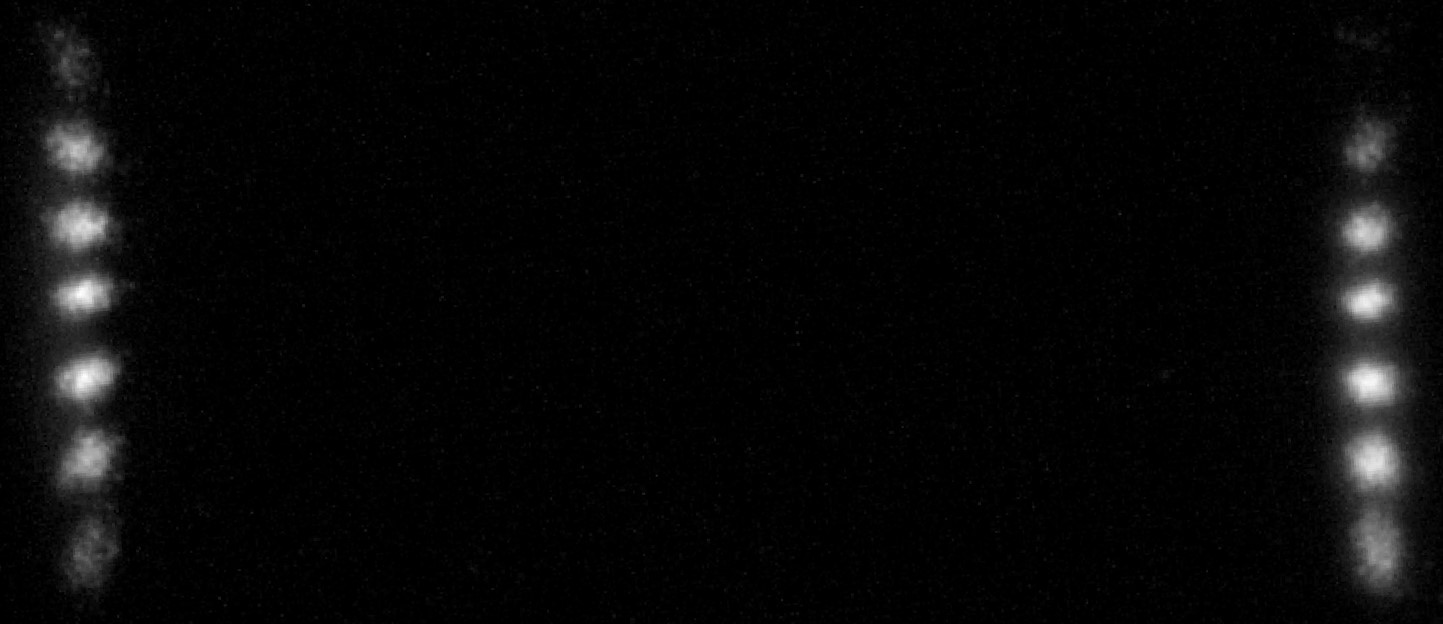
\includegraphics[width=0.5\linewidth]{part2/Figs/example_calibration.jpeg}
    \caption{An example image used to calibration the timing of the streaked pepperpots.}
    \label{figure:example_calibration}
\end{figure}

\subsection{Pepperpots}
There were a number of iterations on the precise configuration of the one- and two-dimensional pepperpots used in these experiments.
There are a number of considerations when designing pepperpot masks;
\begin{itemize}
    \item{\emph{Aperture size:} Smaller apertures provide a higher resolution to the emittance measurement but reduce the signal as fewer particles pass through the hole.
    Smaller apertures also allow for a smaller aperture spacing as when the aperture diameter and aperture spacing are similar the pepperpot can become fragile.}
    \item{\emph{Aperture spacing:} Aperture spacing, or pitch, determines how well the full beam is sampled.
    Smaller pitch allows for better sampling of the full beam however pitch should be large enough that the beamlets produced from each aperture should not overlap on the detector.
    If the pitch is too small then the pepperpot can also become fragile.}
    \item{\emph{Extent:} Ideally a the total extend of the pepperpot should be much larger than the largest beam for a particular apparatus.
    Unfortunately the Melbourne \gls{caeis} was limited to \unit[3]{mm} diameter, thin samples where a portion of the sample was obscured by the sample holder, as shown in Figure~\ref{figure:sample_holder_pepperpots}.}
\end{itemize}

A number of restrictions aided the selection of parameters for the pepperpots used, the maximum pepperpot extent and need to focus the beam to the pepperpot size to maximise flux dictated the approximate size of the beamlets on the detector and thus the lowest feasibly pitch.
The pepperpots were cut\footnote{The pepperpots were cut using a Oxford Laser Systems Alpha 532 laser micromachining system.} from \unit[25]{$\mu m$} thick copper pinholes\footnote{Gilder Grids GA50-C3, \unit[50]{$\mu m$} aperture.} with \unit[50]{$\mu m$} diameter holes cut in the centre.
The central pinholes were used as the central aperture for the pepperpot arrays and since \unit[50]{$\mu m$} apertures provide adequate flux the rest of the apertures were also cut to the same diameter to simplify analysis.

\begin{figure}
    \center
    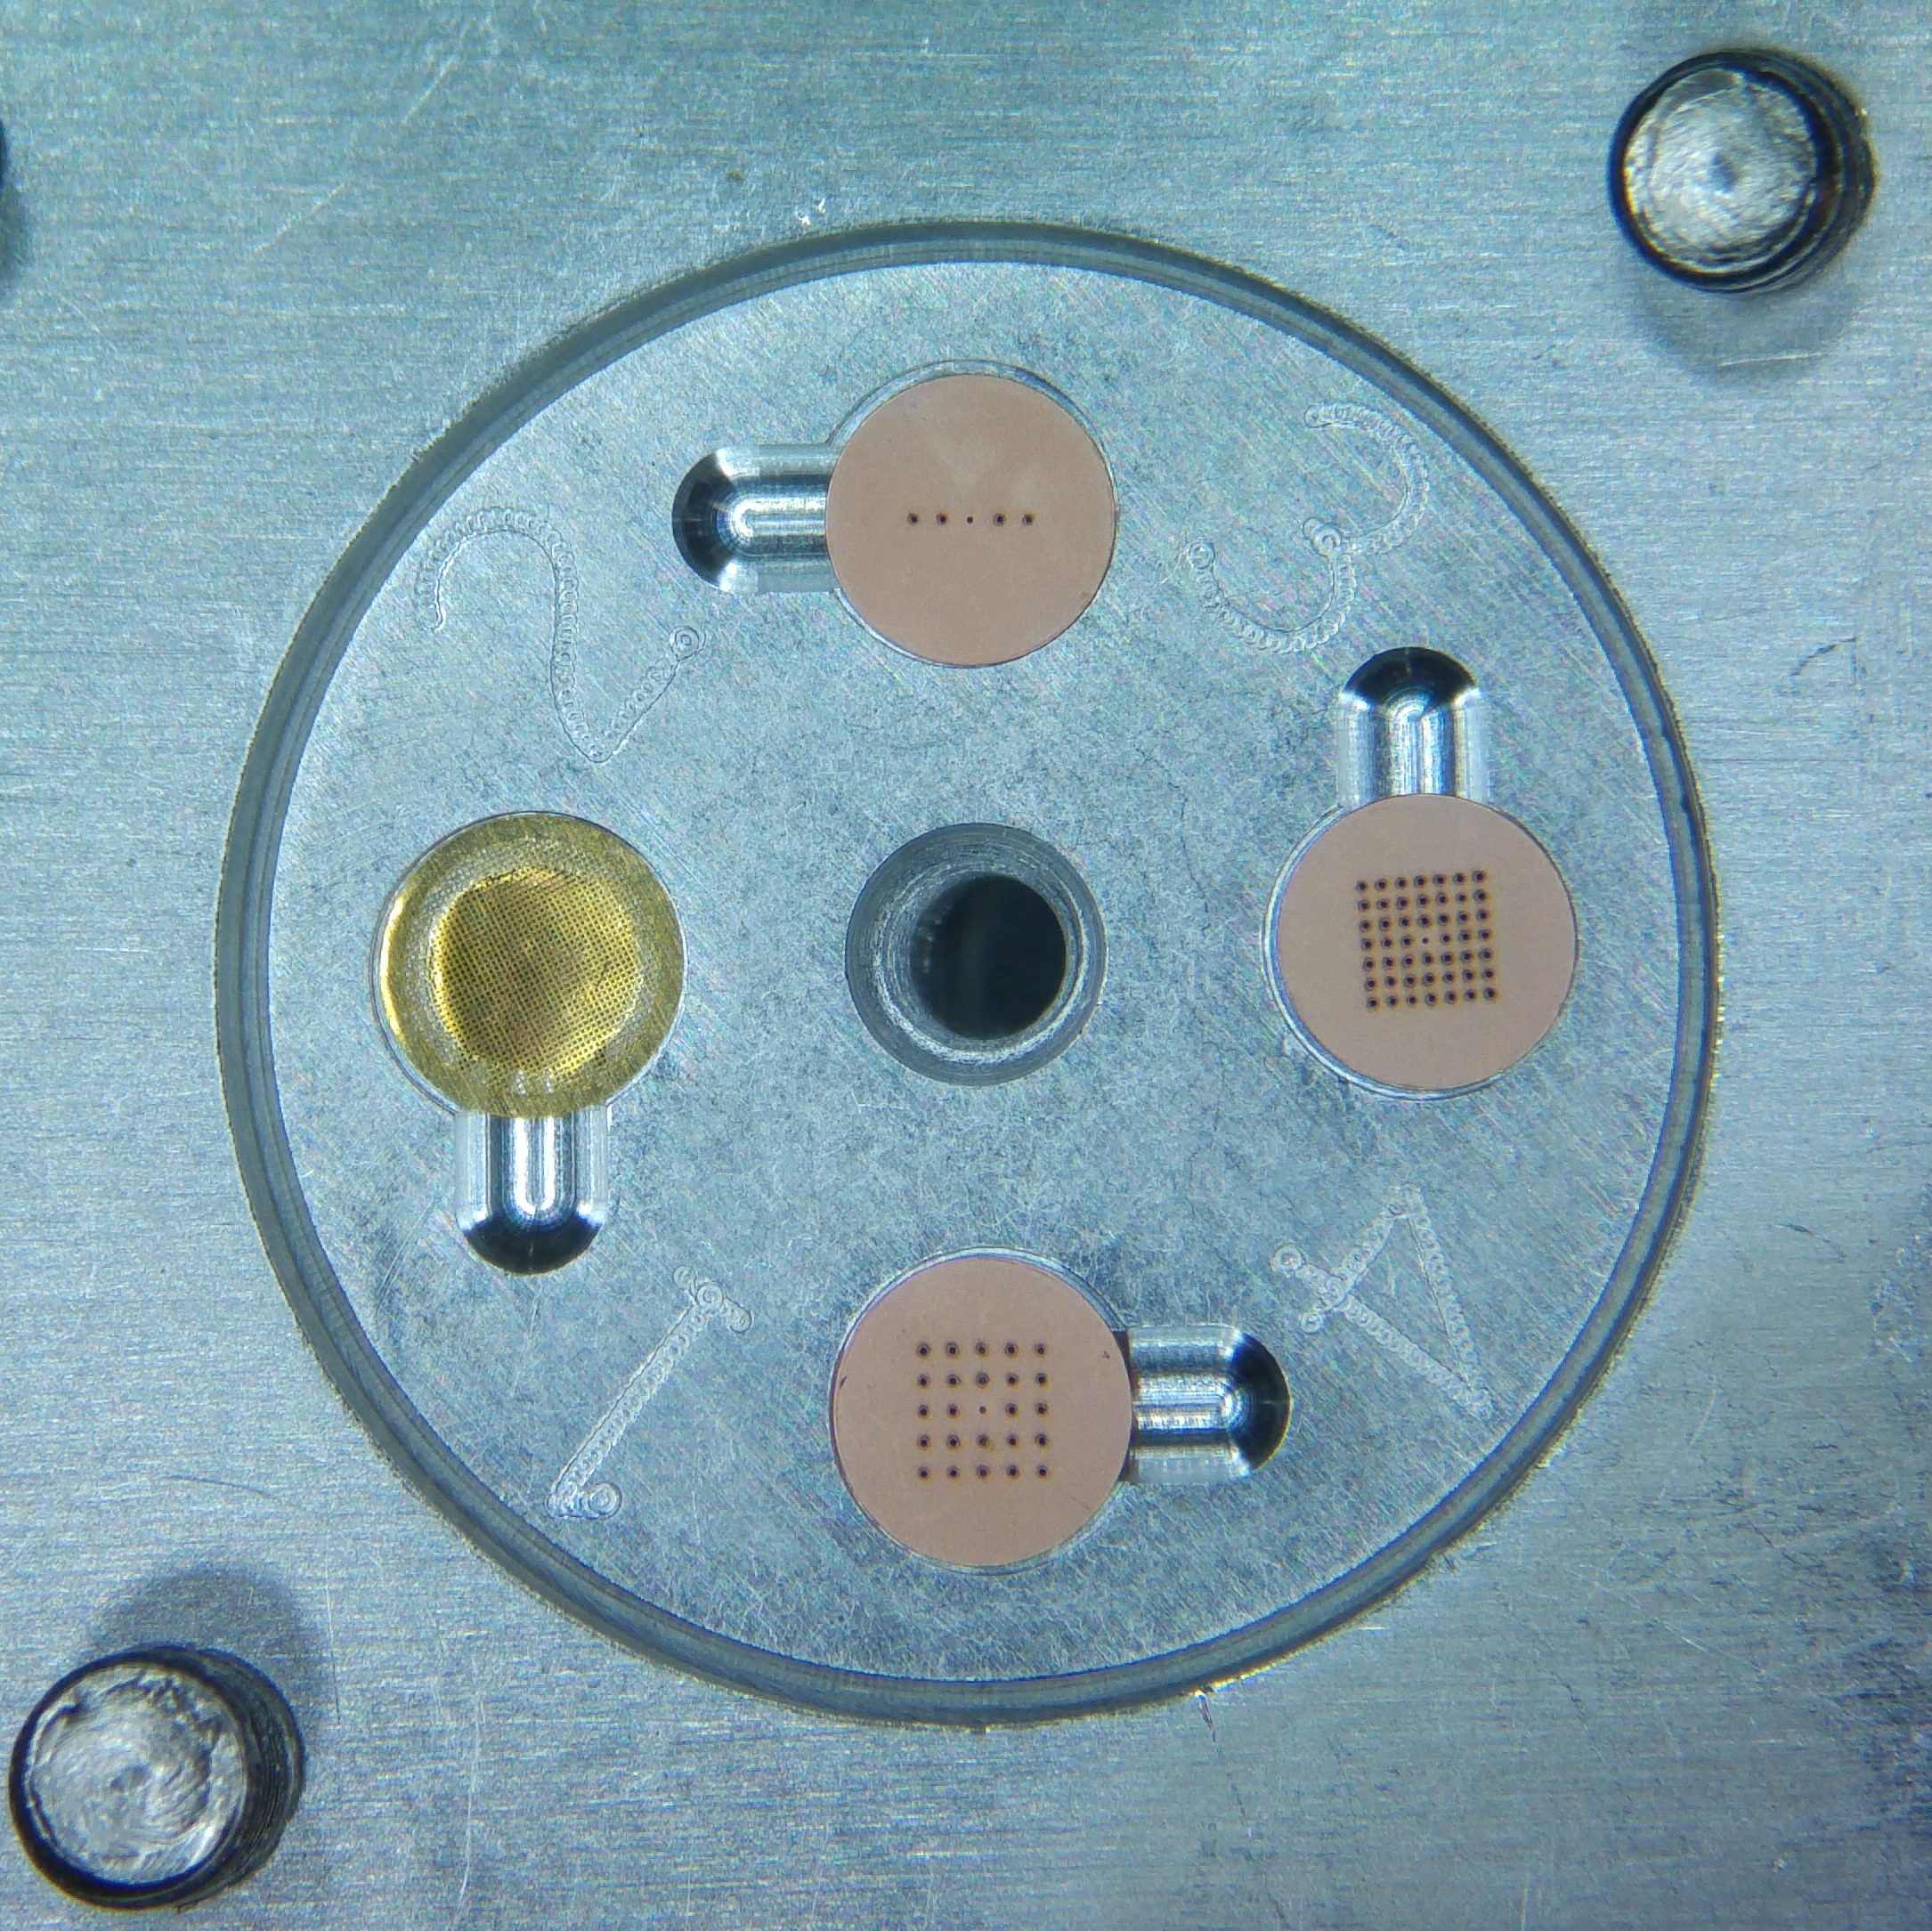
\includegraphics[width=0.49\linewidth]{part2/Figs/sample_holder.jpg}
    \caption{One of two sampleholders that are used to load up to eight samples into the vacuum system. Clockwise from the top: five \unit[50]{$\mu m$} apertures with \unit[300]{$\mu m$} pitch, 7 by 7 pepperpot of \unit[50]{$\mu m$} apertures with \unit[200]{$\mu m$} pitch, 5 by 5 pepperpot of \unit[50]{$\mu m$} apertures with \unit[300]{$\mu m$} pitch, thin gold sample. Each sample is \unit[3]{mm} in diameter. A `lid' with appropriate apertures is placed over the samples to hold them in place.}
    \label{figure:sample_holder_pepperpots}
\end{figure}

\subsection{Laser Parameters}
Two of the lasers essential to the functioning are the `excitation' and `ionisation' lasers, see Section~\ref{section:two_stage_ionisation}, a CW red and pulsed blue laser respectively.
These lasers have a number of parameters that affect the emittance measurements.

\subsubsection{Excitation Laser}
The excitation laser was a \unit[780]{nm} laser, frequency locked to the Rb85 D2 F=3 to F=4 transition, which excites ground state atoms in the \gls{mot} to prepare the atoms for ionisation.
The spatial profile of this laser is highly controllable with a \gls{slm} allowing for arbitrary profiles to be mapped to the electron or ion bunch~\cite{mcculloch_arbitrarily_2011}.
The highest flux is possible by simply saturating the \gls{mot} however control over the electron beam profile and size is usually desirable.
One commonly used and simple distribution is a flat-top distribution as it can provide even electron intensity across the sample under examination however electron beams generated from electrons with high excess energy are unable to maintain the distribution, see Figure~\ref{figure:flat_top}.

\begin{figure}
    \center
    %% Creator: Matplotlib, PGF backend
%%
%% To include the figure in your LaTeX document, write
%%   \input{<filename>.pgf}
%%
%% Make sure the required packages are loaded in your preamble
%%   \usepackage{pgf}
%%
%% Figures using additional raster images can only be included by \input if
%% they are in the same directory as the main LaTeX file. For loading figures
%% from other directories you can use the `import` package
%%   \usepackage{import}
%% and then include the figures with
%%   \import{<path to file>}{<filename>.pgf}
%%
%% Matplotlib used the following preamble
%%
\begingroup%
\makeatletter%
\begin{pgfpicture}%
\pgfpathrectangle{\pgfpointorigin}{\pgfqpoint{5.424500in}{3.977967in}}%
\pgfusepath{use as bounding box, clip}%
\begin{pgfscope}%
\pgfsetbuttcap%
\pgfsetmiterjoin%
\definecolor{currentfill}{rgb}{1.000000,1.000000,1.000000}%
\pgfsetfillcolor{currentfill}%
\pgfsetlinewidth{0.000000pt}%
\definecolor{currentstroke}{rgb}{1.000000,1.000000,1.000000}%
\pgfsetstrokecolor{currentstroke}%
\pgfsetdash{}{0pt}%
\pgfpathmoveto{\pgfqpoint{0.000000in}{0.000000in}}%
\pgfpathlineto{\pgfqpoint{5.424500in}{0.000000in}}%
\pgfpathlineto{\pgfqpoint{5.424500in}{3.977967in}}%
\pgfpathlineto{\pgfqpoint{0.000000in}{3.977967in}}%
\pgfpathclose%
\pgfusepath{fill}%
\end{pgfscope}%
\begin{pgfscope}%
\pgfsetbuttcap%
\pgfsetmiterjoin%
\definecolor{currentfill}{rgb}{1.000000,1.000000,1.000000}%
\pgfsetfillcolor{currentfill}%
\pgfsetlinewidth{0.000000pt}%
\definecolor{currentstroke}{rgb}{0.000000,0.000000,0.000000}%
\pgfsetstrokecolor{currentstroke}%
\pgfsetstrokeopacity{0.000000}%
\pgfsetdash{}{0pt}%
\pgfpathmoveto{\pgfqpoint{0.396944in}{2.104261in}}%
\pgfpathlineto{\pgfqpoint{2.017796in}{2.104261in}}%
\pgfpathlineto{\pgfqpoint{2.017796in}{3.593522in}}%
\pgfpathlineto{\pgfqpoint{0.396944in}{3.593522in}}%
\pgfpathclose%
\pgfusepath{fill}%
\end{pgfscope}%
\begin{pgfscope}%
\pgfpathrectangle{\pgfqpoint{0.396944in}{2.104261in}}{\pgfqpoint{1.620852in}{1.489261in}} %
\pgfusepath{clip}%
\pgftext[at=\pgfqpoint{0.396944in}{2.104261in},left,bottom]{\pgfimage[interpolate=true,width=1.630000in,height=1.500000in]{flattops_emittance-img0.png}}%
\end{pgfscope}%
\begin{pgfscope}%
\pgfpathrectangle{\pgfqpoint{0.396944in}{2.104261in}}{\pgfqpoint{1.620852in}{1.489261in}} %
\pgfusepath{clip}%
\pgfsetbuttcap%
\pgfsetroundjoin%
\pgfsetlinewidth{1.003750pt}%
\definecolor{currentstroke}{rgb}{1.000000,1.000000,1.000000}%
\pgfsetstrokecolor{currentstroke}%
\pgfsetdash{{6.000000pt}{6.000000pt}}{0.000000pt}%
\pgfpathmoveto{\pgfqpoint{0.396944in}{2.846410in}}%
\pgfpathlineto{\pgfqpoint{2.017796in}{2.846410in}}%
\pgfusepath{stroke}%
\end{pgfscope}%
\begin{pgfscope}%
\pgfsetrectcap%
\pgfsetmiterjoin%
\pgfsetlinewidth{1.003750pt}%
\definecolor{currentstroke}{rgb}{0.000000,0.000000,0.000000}%
\pgfsetstrokecolor{currentstroke}%
\pgfsetdash{}{0pt}%
\pgfpathmoveto{\pgfqpoint{0.396944in}{2.104261in}}%
\pgfpathlineto{\pgfqpoint{0.396944in}{3.593522in}}%
\pgfusepath{stroke}%
\end{pgfscope}%
\begin{pgfscope}%
\pgfsetrectcap%
\pgfsetmiterjoin%
\pgfsetlinewidth{1.003750pt}%
\definecolor{currentstroke}{rgb}{0.000000,0.000000,0.000000}%
\pgfsetstrokecolor{currentstroke}%
\pgfsetdash{}{0pt}%
\pgfpathmoveto{\pgfqpoint{0.396944in}{2.104261in}}%
\pgfpathlineto{\pgfqpoint{2.017796in}{2.104261in}}%
\pgfusepath{stroke}%
\end{pgfscope}%
\begin{pgfscope}%
\pgfsetrectcap%
\pgfsetmiterjoin%
\pgfsetlinewidth{1.003750pt}%
\definecolor{currentstroke}{rgb}{0.000000,0.000000,0.000000}%
\pgfsetstrokecolor{currentstroke}%
\pgfsetdash{}{0pt}%
\pgfpathmoveto{\pgfqpoint{0.396944in}{3.593522in}}%
\pgfpathlineto{\pgfqpoint{2.017796in}{3.593522in}}%
\pgfusepath{stroke}%
\end{pgfscope}%
\begin{pgfscope}%
\pgfsetrectcap%
\pgfsetmiterjoin%
\pgfsetlinewidth{1.003750pt}%
\definecolor{currentstroke}{rgb}{0.000000,0.000000,0.000000}%
\pgfsetstrokecolor{currentstroke}%
\pgfsetdash{}{0pt}%
\pgfpathmoveto{\pgfqpoint{2.017796in}{2.104261in}}%
\pgfpathlineto{\pgfqpoint{2.017796in}{3.593522in}}%
\pgfusepath{stroke}%
\end{pgfscope}%
\begin{pgfscope}%
\pgftext[x=1.207370in,y=3.662967in,,base]{\rmfamily\fontsize{13.200000}{15.840000}\selectfont -42.0\(\displaystyle \,\)meV}%
\end{pgfscope}%
\begin{pgfscope}%
\pgfsetbuttcap%
\pgfsetmiterjoin%
\definecolor{currentfill}{rgb}{1.000000,1.000000,1.000000}%
\pgfsetfillcolor{currentfill}%
\pgfsetlinewidth{0.000000pt}%
\definecolor{currentstroke}{rgb}{0.000000,0.000000,0.000000}%
\pgfsetstrokecolor{currentstroke}%
\pgfsetstrokeopacity{0.000000}%
\pgfsetdash{}{0pt}%
\pgfpathmoveto{\pgfqpoint{0.396944in}{0.615000in}}%
\pgfpathlineto{\pgfqpoint{2.017796in}{0.615000in}}%
\pgfpathlineto{\pgfqpoint{2.017796in}{2.104261in}}%
\pgfpathlineto{\pgfqpoint{0.396944in}{2.104261in}}%
\pgfpathclose%
\pgfusepath{fill}%
\end{pgfscope}%
\begin{pgfscope}%
\pgfpathrectangle{\pgfqpoint{0.396944in}{0.615000in}}{\pgfqpoint{1.620852in}{1.489261in}} %
\pgfusepath{clip}%
\pgfsetbuttcap%
\pgfsetroundjoin%
\pgfsetlinewidth{1.003750pt}%
\definecolor{currentstroke}{rgb}{1.000000,0.000000,0.000000}%
\pgfsetstrokecolor{currentstroke}%
\pgfsetdash{{1.000000pt}{3.000000pt}}{0.000000pt}%
\pgfpathmoveto{\pgfqpoint{0.396944in}{0.624506in}}%
\pgfpathlineto{\pgfqpoint{0.402347in}{0.617183in}}%
\pgfpathlineto{\pgfqpoint{0.407750in}{0.615000in}}%
\pgfpathlineto{\pgfqpoint{0.413153in}{0.615830in}}%
\pgfpathlineto{\pgfqpoint{0.418556in}{0.618413in}}%
\pgfpathlineto{\pgfqpoint{0.434764in}{0.633164in}}%
\pgfpathlineto{\pgfqpoint{0.445570in}{0.631717in}}%
\pgfpathlineto{\pgfqpoint{0.450973in}{0.629860in}}%
\pgfpathlineto{\pgfqpoint{0.456376in}{0.633103in}}%
\pgfpathlineto{\pgfqpoint{0.461779in}{0.641380in}}%
\pgfpathlineto{\pgfqpoint{0.472584in}{0.653406in}}%
\pgfpathlineto{\pgfqpoint{0.477987in}{0.663637in}}%
\pgfpathlineto{\pgfqpoint{0.488793in}{0.674176in}}%
\pgfpathlineto{\pgfqpoint{0.494196in}{0.674855in}}%
\pgfpathlineto{\pgfqpoint{0.499598in}{0.680154in}}%
\pgfpathlineto{\pgfqpoint{0.505001in}{0.682156in}}%
\pgfpathlineto{\pgfqpoint{0.510404in}{0.692276in}}%
\pgfpathlineto{\pgfqpoint{0.515807in}{0.698970in}}%
\pgfpathlineto{\pgfqpoint{0.521210in}{0.701174in}}%
\pgfpathlineto{\pgfqpoint{0.532015in}{0.725330in}}%
\pgfpathlineto{\pgfqpoint{0.542821in}{0.753712in}}%
\pgfpathlineto{\pgfqpoint{0.548224in}{0.764961in}}%
\pgfpathlineto{\pgfqpoint{0.559030in}{0.773106in}}%
\pgfpathlineto{\pgfqpoint{0.564432in}{0.782553in}}%
\pgfpathlineto{\pgfqpoint{0.569835in}{0.795326in}}%
\pgfpathlineto{\pgfqpoint{0.580641in}{0.828780in}}%
\pgfpathlineto{\pgfqpoint{0.591447in}{0.846073in}}%
\pgfpathlineto{\pgfqpoint{0.596850in}{0.848364in}}%
\pgfpathlineto{\pgfqpoint{0.613058in}{0.908456in}}%
\pgfpathlineto{\pgfqpoint{0.623864in}{0.937368in}}%
\pgfpathlineto{\pgfqpoint{0.629267in}{0.949366in}}%
\pgfpathlineto{\pgfqpoint{0.640072in}{0.984131in}}%
\pgfpathlineto{\pgfqpoint{0.645475in}{0.996817in}}%
\pgfpathlineto{\pgfqpoint{0.650878in}{1.015002in}}%
\pgfpathlineto{\pgfqpoint{0.656281in}{1.023664in}}%
\pgfpathlineto{\pgfqpoint{0.661684in}{1.037305in}}%
\pgfpathlineto{\pgfqpoint{0.667086in}{1.043856in}}%
\pgfpathlineto{\pgfqpoint{0.683295in}{1.095942in}}%
\pgfpathlineto{\pgfqpoint{0.688698in}{1.110675in}}%
\pgfpathlineto{\pgfqpoint{0.694101in}{1.133854in}}%
\pgfpathlineto{\pgfqpoint{0.699503in}{1.144489in}}%
\pgfpathlineto{\pgfqpoint{0.704906in}{1.161049in}}%
\pgfpathlineto{\pgfqpoint{0.710309in}{1.186676in}}%
\pgfpathlineto{\pgfqpoint{0.715712in}{1.198221in}}%
\pgfpathlineto{\pgfqpoint{0.726518in}{1.217748in}}%
\pgfpathlineto{\pgfqpoint{0.731920in}{1.247198in}}%
\pgfpathlineto{\pgfqpoint{0.742726in}{1.291361in}}%
\pgfpathlineto{\pgfqpoint{0.753532in}{1.329699in}}%
\pgfpathlineto{\pgfqpoint{0.758935in}{1.330222in}}%
\pgfpathlineto{\pgfqpoint{0.764338in}{1.337509in}}%
\pgfpathlineto{\pgfqpoint{0.769740in}{1.352766in}}%
\pgfpathlineto{\pgfqpoint{0.775143in}{1.377587in}}%
\pgfpathlineto{\pgfqpoint{0.780546in}{1.395487in}}%
\pgfpathlineto{\pgfqpoint{0.785949in}{1.425367in}}%
\pgfpathlineto{\pgfqpoint{0.791352in}{1.447276in}}%
\pgfpathlineto{\pgfqpoint{0.796755in}{1.454341in}}%
\pgfpathlineto{\pgfqpoint{0.802157in}{1.456747in}}%
\pgfpathlineto{\pgfqpoint{0.807560in}{1.466169in}}%
\pgfpathlineto{\pgfqpoint{0.812963in}{1.478067in}}%
\pgfpathlineto{\pgfqpoint{0.818366in}{1.500692in}}%
\pgfpathlineto{\pgfqpoint{0.823769in}{1.506510in}}%
\pgfpathlineto{\pgfqpoint{0.834574in}{1.500069in}}%
\pgfpathlineto{\pgfqpoint{0.845380in}{1.517184in}}%
\pgfpathlineto{\pgfqpoint{0.861589in}{1.609881in}}%
\pgfpathlineto{\pgfqpoint{0.872394in}{1.625364in}}%
\pgfpathlineto{\pgfqpoint{0.877797in}{1.641911in}}%
\pgfpathlineto{\pgfqpoint{0.883200in}{1.676034in}}%
\pgfpathlineto{\pgfqpoint{0.888603in}{1.696906in}}%
\pgfpathlineto{\pgfqpoint{0.904811in}{1.705828in}}%
\pgfpathlineto{\pgfqpoint{0.910214in}{1.698244in}}%
\pgfpathlineto{\pgfqpoint{0.915617in}{1.704252in}}%
\pgfpathlineto{\pgfqpoint{0.921020in}{1.717012in}}%
\pgfpathlineto{\pgfqpoint{0.926423in}{1.746840in}}%
\pgfpathlineto{\pgfqpoint{0.931826in}{1.743679in}}%
\pgfpathlineto{\pgfqpoint{0.937228in}{1.742522in}}%
\pgfpathlineto{\pgfqpoint{0.942631in}{1.723305in}}%
\pgfpathlineto{\pgfqpoint{0.948034in}{1.711510in}}%
\pgfpathlineto{\pgfqpoint{0.953437in}{1.731151in}}%
\pgfpathlineto{\pgfqpoint{0.964243in}{1.758237in}}%
\pgfpathlineto{\pgfqpoint{0.969645in}{1.770696in}}%
\pgfpathlineto{\pgfqpoint{0.975048in}{1.763072in}}%
\pgfpathlineto{\pgfqpoint{0.980451in}{1.743022in}}%
\pgfpathlineto{\pgfqpoint{0.985854in}{1.741979in}}%
\pgfpathlineto{\pgfqpoint{0.991257in}{1.768678in}}%
\pgfpathlineto{\pgfqpoint{1.002062in}{1.804722in}}%
\pgfpathlineto{\pgfqpoint{1.012868in}{1.800859in}}%
\pgfpathlineto{\pgfqpoint{1.018271in}{1.804120in}}%
\pgfpathlineto{\pgfqpoint{1.023674in}{1.809490in}}%
\pgfpathlineto{\pgfqpoint{1.029077in}{1.830170in}}%
\pgfpathlineto{\pgfqpoint{1.034480in}{1.855304in}}%
\pgfpathlineto{\pgfqpoint{1.039882in}{1.850514in}}%
\pgfpathlineto{\pgfqpoint{1.045285in}{1.849056in}}%
\pgfpathlineto{\pgfqpoint{1.050688in}{1.845176in}}%
\pgfpathlineto{\pgfqpoint{1.056091in}{1.847910in}}%
\pgfpathlineto{\pgfqpoint{1.066897in}{1.918792in}}%
\pgfpathlineto{\pgfqpoint{1.072299in}{1.936413in}}%
\pgfpathlineto{\pgfqpoint{1.077702in}{1.942640in}}%
\pgfpathlineto{\pgfqpoint{1.083105in}{1.919165in}}%
\pgfpathlineto{\pgfqpoint{1.088508in}{1.929888in}}%
\pgfpathlineto{\pgfqpoint{1.093911in}{1.949997in}}%
\pgfpathlineto{\pgfqpoint{1.099314in}{1.984919in}}%
\pgfpathlineto{\pgfqpoint{1.104716in}{1.997039in}}%
\pgfpathlineto{\pgfqpoint{1.110119in}{1.985391in}}%
\pgfpathlineto{\pgfqpoint{1.115522in}{1.979564in}}%
\pgfpathlineto{\pgfqpoint{1.120925in}{1.993797in}}%
\pgfpathlineto{\pgfqpoint{1.131731in}{2.014487in}}%
\pgfpathlineto{\pgfqpoint{1.137133in}{2.028705in}}%
\pgfpathlineto{\pgfqpoint{1.147939in}{2.005485in}}%
\pgfpathlineto{\pgfqpoint{1.153342in}{1.978272in}}%
\pgfpathlineto{\pgfqpoint{1.158745in}{1.991513in}}%
\pgfpathlineto{\pgfqpoint{1.164148in}{1.999734in}}%
\pgfpathlineto{\pgfqpoint{1.169550in}{2.021193in}}%
\pgfpathlineto{\pgfqpoint{1.174953in}{2.033344in}}%
\pgfpathlineto{\pgfqpoint{1.180356in}{2.021453in}}%
\pgfpathlineto{\pgfqpoint{1.191162in}{1.975564in}}%
\pgfpathlineto{\pgfqpoint{1.196565in}{1.979900in}}%
\pgfpathlineto{\pgfqpoint{1.201968in}{1.996861in}}%
\pgfpathlineto{\pgfqpoint{1.207370in}{2.017661in}}%
\pgfpathlineto{\pgfqpoint{1.218176in}{2.001975in}}%
\pgfpathlineto{\pgfqpoint{1.228982in}{1.963851in}}%
\pgfpathlineto{\pgfqpoint{1.234385in}{1.983969in}}%
\pgfpathlineto{\pgfqpoint{1.239787in}{2.015341in}}%
\pgfpathlineto{\pgfqpoint{1.245190in}{2.015105in}}%
\pgfpathlineto{\pgfqpoint{1.250593in}{1.986095in}}%
\pgfpathlineto{\pgfqpoint{1.261399in}{1.953630in}}%
\pgfpathlineto{\pgfqpoint{1.266802in}{1.949386in}}%
\pgfpathlineto{\pgfqpoint{1.272204in}{1.966186in}}%
\pgfpathlineto{\pgfqpoint{1.277607in}{1.958593in}}%
\pgfpathlineto{\pgfqpoint{1.283010in}{1.955774in}}%
\pgfpathlineto{\pgfqpoint{1.293816in}{1.916153in}}%
\pgfpathlineto{\pgfqpoint{1.299219in}{1.912828in}}%
\pgfpathlineto{\pgfqpoint{1.304621in}{1.916281in}}%
\pgfpathlineto{\pgfqpoint{1.310024in}{1.929046in}}%
\pgfpathlineto{\pgfqpoint{1.320830in}{1.911792in}}%
\pgfpathlineto{\pgfqpoint{1.331636in}{1.881268in}}%
\pgfpathlineto{\pgfqpoint{1.337039in}{1.890023in}}%
\pgfpathlineto{\pgfqpoint{1.342441in}{1.905559in}}%
\pgfpathlineto{\pgfqpoint{1.347844in}{1.914307in}}%
\pgfpathlineto{\pgfqpoint{1.358650in}{1.901259in}}%
\pgfpathlineto{\pgfqpoint{1.364053in}{1.879160in}}%
\pgfpathlineto{\pgfqpoint{1.369456in}{1.868038in}}%
\pgfpathlineto{\pgfqpoint{1.374858in}{1.869194in}}%
\pgfpathlineto{\pgfqpoint{1.380261in}{1.891658in}}%
\pgfpathlineto{\pgfqpoint{1.385664in}{1.898922in}}%
\pgfpathlineto{\pgfqpoint{1.391067in}{1.884713in}}%
\pgfpathlineto{\pgfqpoint{1.396470in}{1.850157in}}%
\pgfpathlineto{\pgfqpoint{1.401873in}{1.825040in}}%
\pgfpathlineto{\pgfqpoint{1.407275in}{1.821226in}}%
\pgfpathlineto{\pgfqpoint{1.412678in}{1.826164in}}%
\pgfpathlineto{\pgfqpoint{1.418081in}{1.814499in}}%
\pgfpathlineto{\pgfqpoint{1.423484in}{1.806746in}}%
\pgfpathlineto{\pgfqpoint{1.428887in}{1.786458in}}%
\pgfpathlineto{\pgfqpoint{1.439692in}{1.717497in}}%
\pgfpathlineto{\pgfqpoint{1.445095in}{1.736045in}}%
\pgfpathlineto{\pgfqpoint{1.455901in}{1.783806in}}%
\pgfpathlineto{\pgfqpoint{1.461304in}{1.778362in}}%
\pgfpathlineto{\pgfqpoint{1.466707in}{1.759812in}}%
\pgfpathlineto{\pgfqpoint{1.472110in}{1.725997in}}%
\pgfpathlineto{\pgfqpoint{1.477512in}{1.745386in}}%
\pgfpathlineto{\pgfqpoint{1.482915in}{1.737790in}}%
\pgfpathlineto{\pgfqpoint{1.488318in}{1.726730in}}%
\pgfpathlineto{\pgfqpoint{1.499124in}{1.692137in}}%
\pgfpathlineto{\pgfqpoint{1.504527in}{1.657320in}}%
\pgfpathlineto{\pgfqpoint{1.515332in}{1.611988in}}%
\pgfpathlineto{\pgfqpoint{1.520735in}{1.620910in}}%
\pgfpathlineto{\pgfqpoint{1.526138in}{1.609485in}}%
\pgfpathlineto{\pgfqpoint{1.531541in}{1.592182in}}%
\pgfpathlineto{\pgfqpoint{1.536944in}{1.565616in}}%
\pgfpathlineto{\pgfqpoint{1.542346in}{1.530017in}}%
\pgfpathlineto{\pgfqpoint{1.547749in}{1.513145in}}%
\pgfpathlineto{\pgfqpoint{1.553152in}{1.506941in}}%
\pgfpathlineto{\pgfqpoint{1.563958in}{1.488595in}}%
\pgfpathlineto{\pgfqpoint{1.569361in}{1.490645in}}%
\pgfpathlineto{\pgfqpoint{1.580166in}{1.446096in}}%
\pgfpathlineto{\pgfqpoint{1.585569in}{1.435569in}}%
\pgfpathlineto{\pgfqpoint{1.590972in}{1.434589in}}%
\pgfpathlineto{\pgfqpoint{1.596375in}{1.426068in}}%
\pgfpathlineto{\pgfqpoint{1.601778in}{1.413680in}}%
\pgfpathlineto{\pgfqpoint{1.607180in}{1.389409in}}%
\pgfpathlineto{\pgfqpoint{1.617986in}{1.325803in}}%
\pgfpathlineto{\pgfqpoint{1.623389in}{1.309119in}}%
\pgfpathlineto{\pgfqpoint{1.645000in}{1.228860in}}%
\pgfpathlineto{\pgfqpoint{1.650403in}{1.198382in}}%
\pgfpathlineto{\pgfqpoint{1.655806in}{1.174633in}}%
\pgfpathlineto{\pgfqpoint{1.661209in}{1.160604in}}%
\pgfpathlineto{\pgfqpoint{1.672015in}{1.120440in}}%
\pgfpathlineto{\pgfqpoint{1.677417in}{1.107922in}}%
\pgfpathlineto{\pgfqpoint{1.682820in}{1.089267in}}%
\pgfpathlineto{\pgfqpoint{1.688223in}{1.094514in}}%
\pgfpathlineto{\pgfqpoint{1.693626in}{1.083771in}}%
\pgfpathlineto{\pgfqpoint{1.699029in}{1.057427in}}%
\pgfpathlineto{\pgfqpoint{1.709834in}{0.999439in}}%
\pgfpathlineto{\pgfqpoint{1.715237in}{0.990971in}}%
\pgfpathlineto{\pgfqpoint{1.720640in}{0.976461in}}%
\pgfpathlineto{\pgfqpoint{1.731446in}{0.959648in}}%
\pgfpathlineto{\pgfqpoint{1.747654in}{0.905056in}}%
\pgfpathlineto{\pgfqpoint{1.758460in}{0.860632in}}%
\pgfpathlineto{\pgfqpoint{1.763863in}{0.859552in}}%
\pgfpathlineto{\pgfqpoint{1.769266in}{0.843635in}}%
\pgfpathlineto{\pgfqpoint{1.785474in}{0.806525in}}%
\pgfpathlineto{\pgfqpoint{1.790877in}{0.793159in}}%
\pgfpathlineto{\pgfqpoint{1.801683in}{0.779348in}}%
\pgfpathlineto{\pgfqpoint{1.817891in}{0.740778in}}%
\pgfpathlineto{\pgfqpoint{1.823294in}{0.736172in}}%
\pgfpathlineto{\pgfqpoint{1.828697in}{0.735359in}}%
\pgfpathlineto{\pgfqpoint{1.839503in}{0.738763in}}%
\pgfpathlineto{\pgfqpoint{1.844905in}{0.729006in}}%
\pgfpathlineto{\pgfqpoint{1.850308in}{0.725054in}}%
\pgfpathlineto{\pgfqpoint{1.861114in}{0.727545in}}%
\pgfpathlineto{\pgfqpoint{1.866517in}{0.726100in}}%
\pgfpathlineto{\pgfqpoint{1.871920in}{0.723010in}}%
\pgfpathlineto{\pgfqpoint{1.877322in}{0.713266in}}%
\pgfpathlineto{\pgfqpoint{1.882725in}{0.706297in}}%
\pgfpathlineto{\pgfqpoint{1.888128in}{0.694800in}}%
\pgfpathlineto{\pgfqpoint{1.893531in}{0.686121in}}%
\pgfpathlineto{\pgfqpoint{1.898934in}{0.683309in}}%
\pgfpathlineto{\pgfqpoint{1.904337in}{0.683408in}}%
\pgfpathlineto{\pgfqpoint{1.915142in}{0.673374in}}%
\pgfpathlineto{\pgfqpoint{1.920545in}{0.670289in}}%
\pgfpathlineto{\pgfqpoint{1.925948in}{0.664697in}}%
\pgfpathlineto{\pgfqpoint{1.931351in}{0.664232in}}%
\pgfpathlineto{\pgfqpoint{1.936754in}{0.670154in}}%
\pgfpathlineto{\pgfqpoint{1.942157in}{0.678123in}}%
\pgfpathlineto{\pgfqpoint{1.947559in}{0.681880in}}%
\pgfpathlineto{\pgfqpoint{1.952962in}{0.679534in}}%
\pgfpathlineto{\pgfqpoint{1.958365in}{0.674227in}}%
\pgfpathlineto{\pgfqpoint{1.963768in}{0.666296in}}%
\pgfpathlineto{\pgfqpoint{1.969171in}{0.673768in}}%
\pgfpathlineto{\pgfqpoint{1.974574in}{0.684694in}}%
\pgfpathlineto{\pgfqpoint{1.979976in}{0.685555in}}%
\pgfpathlineto{\pgfqpoint{1.985379in}{0.681985in}}%
\pgfpathlineto{\pgfqpoint{1.990782in}{0.672626in}}%
\pgfpathlineto{\pgfqpoint{1.996185in}{0.666338in}}%
\pgfpathlineto{\pgfqpoint{2.012393in}{0.665880in}}%
\pgfpathlineto{\pgfqpoint{2.012393in}{0.665880in}}%
\pgfusepath{stroke}%
\end{pgfscope}%
\begin{pgfscope}%
\pgfpathrectangle{\pgfqpoint{0.396944in}{0.615000in}}{\pgfqpoint{1.620852in}{1.489261in}} %
\pgfusepath{clip}%
\pgfsetrectcap%
\pgfsetroundjoin%
\pgfsetlinewidth{1.003750pt}%
\definecolor{currentstroke}{rgb}{0.000000,0.000000,1.000000}%
\pgfsetstrokecolor{currentstroke}%
\pgfsetdash{}{0pt}%
\pgfpathmoveto{\pgfqpoint{0.396944in}{0.615000in}}%
\pgfpathlineto{\pgfqpoint{0.402347in}{0.618912in}}%
\pgfpathlineto{\pgfqpoint{0.407750in}{0.619150in}}%
\pgfpathlineto{\pgfqpoint{0.413153in}{0.621395in}}%
\pgfpathlineto{\pgfqpoint{0.423959in}{0.622383in}}%
\pgfpathlineto{\pgfqpoint{0.434764in}{0.619500in}}%
\pgfpathlineto{\pgfqpoint{0.450973in}{0.624916in}}%
\pgfpathlineto{\pgfqpoint{0.456376in}{0.621067in}}%
\pgfpathlineto{\pgfqpoint{0.461779in}{0.621715in}}%
\pgfpathlineto{\pgfqpoint{0.467181in}{0.624334in}}%
\pgfpathlineto{\pgfqpoint{0.472584in}{0.622872in}}%
\pgfpathlineto{\pgfqpoint{0.483390in}{0.623885in}}%
\pgfpathlineto{\pgfqpoint{0.488793in}{0.628712in}}%
\pgfpathlineto{\pgfqpoint{0.494196in}{0.630422in}}%
\pgfpathlineto{\pgfqpoint{0.510404in}{0.631175in}}%
\pgfpathlineto{\pgfqpoint{0.515807in}{0.639049in}}%
\pgfpathlineto{\pgfqpoint{0.521210in}{0.638590in}}%
\pgfpathlineto{\pgfqpoint{0.537418in}{0.629095in}}%
\pgfpathlineto{\pgfqpoint{0.542821in}{0.629626in}}%
\pgfpathlineto{\pgfqpoint{0.548224in}{0.632354in}}%
\pgfpathlineto{\pgfqpoint{0.553627in}{0.631579in}}%
\pgfpathlineto{\pgfqpoint{0.564432in}{0.643352in}}%
\pgfpathlineto{\pgfqpoint{0.575238in}{0.645350in}}%
\pgfpathlineto{\pgfqpoint{0.596850in}{0.658271in}}%
\pgfpathlineto{\pgfqpoint{0.602252in}{0.659259in}}%
\pgfpathlineto{\pgfqpoint{0.613058in}{0.652909in}}%
\pgfpathlineto{\pgfqpoint{0.623864in}{0.647374in}}%
\pgfpathlineto{\pgfqpoint{0.634669in}{0.653351in}}%
\pgfpathlineto{\pgfqpoint{0.645475in}{0.656883in}}%
\pgfpathlineto{\pgfqpoint{0.661684in}{0.669351in}}%
\pgfpathlineto{\pgfqpoint{0.672489in}{0.664428in}}%
\pgfpathlineto{\pgfqpoint{0.688698in}{0.677051in}}%
\pgfpathlineto{\pgfqpoint{0.704906in}{0.692320in}}%
\pgfpathlineto{\pgfqpoint{0.710309in}{0.705349in}}%
\pgfpathlineto{\pgfqpoint{0.715712in}{0.711165in}}%
\pgfpathlineto{\pgfqpoint{0.726518in}{0.726586in}}%
\pgfpathlineto{\pgfqpoint{0.737323in}{0.736936in}}%
\pgfpathlineto{\pgfqpoint{0.742726in}{0.743867in}}%
\pgfpathlineto{\pgfqpoint{0.753532in}{0.764385in}}%
\pgfpathlineto{\pgfqpoint{0.758935in}{0.777190in}}%
\pgfpathlineto{\pgfqpoint{0.769740in}{0.790451in}}%
\pgfpathlineto{\pgfqpoint{0.775143in}{0.800330in}}%
\pgfpathlineto{\pgfqpoint{0.780546in}{0.817574in}}%
\pgfpathlineto{\pgfqpoint{0.785949in}{0.824454in}}%
\pgfpathlineto{\pgfqpoint{0.796755in}{0.881494in}}%
\pgfpathlineto{\pgfqpoint{0.802157in}{0.908844in}}%
\pgfpathlineto{\pgfqpoint{0.807560in}{0.927323in}}%
\pgfpathlineto{\pgfqpoint{0.812963in}{0.941603in}}%
\pgfpathlineto{\pgfqpoint{0.829172in}{1.035107in}}%
\pgfpathlineto{\pgfqpoint{0.839977in}{1.150685in}}%
\pgfpathlineto{\pgfqpoint{0.856186in}{1.276340in}}%
\pgfpathlineto{\pgfqpoint{0.866991in}{1.385634in}}%
\pgfpathlineto{\pgfqpoint{0.899409in}{1.664456in}}%
\pgfpathlineto{\pgfqpoint{0.910214in}{1.714582in}}%
\pgfpathlineto{\pgfqpoint{0.915617in}{1.741586in}}%
\pgfpathlineto{\pgfqpoint{0.921020in}{1.751345in}}%
\pgfpathlineto{\pgfqpoint{0.926423in}{1.765812in}}%
\pgfpathlineto{\pgfqpoint{0.937228in}{1.849557in}}%
\pgfpathlineto{\pgfqpoint{0.942631in}{1.881232in}}%
\pgfpathlineto{\pgfqpoint{0.948034in}{1.874213in}}%
\pgfpathlineto{\pgfqpoint{0.953437in}{1.864884in}}%
\pgfpathlineto{\pgfqpoint{0.958840in}{1.868372in}}%
\pgfpathlineto{\pgfqpoint{0.964243in}{1.909196in}}%
\pgfpathlineto{\pgfqpoint{0.969645in}{1.927995in}}%
\pgfpathlineto{\pgfqpoint{0.975048in}{1.956620in}}%
\pgfpathlineto{\pgfqpoint{0.980451in}{1.961832in}}%
\pgfpathlineto{\pgfqpoint{0.985854in}{1.946864in}}%
\pgfpathlineto{\pgfqpoint{0.991257in}{1.942413in}}%
\pgfpathlineto{\pgfqpoint{0.996660in}{1.941014in}}%
\pgfpathlineto{\pgfqpoint{1.007465in}{1.992551in}}%
\pgfpathlineto{\pgfqpoint{1.012868in}{2.001597in}}%
\pgfpathlineto{\pgfqpoint{1.018271in}{1.990121in}}%
\pgfpathlineto{\pgfqpoint{1.023674in}{1.983319in}}%
\pgfpathlineto{\pgfqpoint{1.029077in}{1.985403in}}%
\pgfpathlineto{\pgfqpoint{1.034480in}{1.989844in}}%
\pgfpathlineto{\pgfqpoint{1.039882in}{2.008424in}}%
\pgfpathlineto{\pgfqpoint{1.045285in}{2.014164in}}%
\pgfpathlineto{\pgfqpoint{1.050688in}{1.990540in}}%
\pgfpathlineto{\pgfqpoint{1.056091in}{1.986105in}}%
\pgfpathlineto{\pgfqpoint{1.061494in}{1.992867in}}%
\pgfpathlineto{\pgfqpoint{1.066897in}{2.002957in}}%
\pgfpathlineto{\pgfqpoint{1.072299in}{2.003725in}}%
\pgfpathlineto{\pgfqpoint{1.077702in}{2.006272in}}%
\pgfpathlineto{\pgfqpoint{1.083105in}{1.996150in}}%
\pgfpathlineto{\pgfqpoint{1.093911in}{1.933907in}}%
\pgfpathlineto{\pgfqpoint{1.099314in}{1.918172in}}%
\pgfpathlineto{\pgfqpoint{1.104716in}{1.922672in}}%
\pgfpathlineto{\pgfqpoint{1.110119in}{1.950718in}}%
\pgfpathlineto{\pgfqpoint{1.115522in}{1.960164in}}%
\pgfpathlineto{\pgfqpoint{1.120925in}{1.955657in}}%
\pgfpathlineto{\pgfqpoint{1.126328in}{1.946150in}}%
\pgfpathlineto{\pgfqpoint{1.131731in}{1.933755in}}%
\pgfpathlineto{\pgfqpoint{1.137133in}{1.935600in}}%
\pgfpathlineto{\pgfqpoint{1.153342in}{1.931738in}}%
\pgfpathlineto{\pgfqpoint{1.158745in}{1.913619in}}%
\pgfpathlineto{\pgfqpoint{1.164148in}{1.888089in}}%
\pgfpathlineto{\pgfqpoint{1.169550in}{1.868714in}}%
\pgfpathlineto{\pgfqpoint{1.174953in}{1.872597in}}%
\pgfpathlineto{\pgfqpoint{1.180356in}{1.904971in}}%
\pgfpathlineto{\pgfqpoint{1.185759in}{1.906235in}}%
\pgfpathlineto{\pgfqpoint{1.196565in}{1.896670in}}%
\pgfpathlineto{\pgfqpoint{1.201968in}{1.879592in}}%
\pgfpathlineto{\pgfqpoint{1.207370in}{1.880253in}}%
\pgfpathlineto{\pgfqpoint{1.212773in}{1.907519in}}%
\pgfpathlineto{\pgfqpoint{1.223579in}{1.946205in}}%
\pgfpathlineto{\pgfqpoint{1.228982in}{1.952248in}}%
\pgfpathlineto{\pgfqpoint{1.239787in}{1.902057in}}%
\pgfpathlineto{\pgfqpoint{1.245190in}{1.917360in}}%
\pgfpathlineto{\pgfqpoint{1.250593in}{1.957087in}}%
\pgfpathlineto{\pgfqpoint{1.255996in}{1.957921in}}%
\pgfpathlineto{\pgfqpoint{1.261399in}{1.951796in}}%
\pgfpathlineto{\pgfqpoint{1.266802in}{1.936372in}}%
\pgfpathlineto{\pgfqpoint{1.272204in}{1.917340in}}%
\pgfpathlineto{\pgfqpoint{1.277607in}{1.931889in}}%
\pgfpathlineto{\pgfqpoint{1.283010in}{1.979207in}}%
\pgfpathlineto{\pgfqpoint{1.288413in}{1.999731in}}%
\pgfpathlineto{\pgfqpoint{1.293816in}{2.007455in}}%
\pgfpathlineto{\pgfqpoint{1.299219in}{1.997185in}}%
\pgfpathlineto{\pgfqpoint{1.304621in}{1.965638in}}%
\pgfpathlineto{\pgfqpoint{1.310024in}{1.971404in}}%
\pgfpathlineto{\pgfqpoint{1.315427in}{1.986499in}}%
\pgfpathlineto{\pgfqpoint{1.320830in}{2.014983in}}%
\pgfpathlineto{\pgfqpoint{1.331636in}{2.030597in}}%
\pgfpathlineto{\pgfqpoint{1.337039in}{2.020350in}}%
\pgfpathlineto{\pgfqpoint{1.342441in}{1.997754in}}%
\pgfpathlineto{\pgfqpoint{1.347844in}{2.004384in}}%
\pgfpathlineto{\pgfqpoint{1.353247in}{2.017365in}}%
\pgfpathlineto{\pgfqpoint{1.358650in}{2.033344in}}%
\pgfpathlineto{\pgfqpoint{1.364053in}{2.024337in}}%
\pgfpathlineto{\pgfqpoint{1.380261in}{1.973106in}}%
\pgfpathlineto{\pgfqpoint{1.385664in}{1.989691in}}%
\pgfpathlineto{\pgfqpoint{1.391067in}{1.999610in}}%
\pgfpathlineto{\pgfqpoint{1.396470in}{2.023655in}}%
\pgfpathlineto{\pgfqpoint{1.401873in}{2.014086in}}%
\pgfpathlineto{\pgfqpoint{1.407275in}{1.983908in}}%
\pgfpathlineto{\pgfqpoint{1.412678in}{1.963635in}}%
\pgfpathlineto{\pgfqpoint{1.418081in}{1.974668in}}%
\pgfpathlineto{\pgfqpoint{1.423484in}{2.000974in}}%
\pgfpathlineto{\pgfqpoint{1.428887in}{2.001001in}}%
\pgfpathlineto{\pgfqpoint{1.445095in}{1.937981in}}%
\pgfpathlineto{\pgfqpoint{1.450498in}{1.928205in}}%
\pgfpathlineto{\pgfqpoint{1.455901in}{1.935924in}}%
\pgfpathlineto{\pgfqpoint{1.461304in}{1.935682in}}%
\pgfpathlineto{\pgfqpoint{1.466707in}{1.895765in}}%
\pgfpathlineto{\pgfqpoint{1.472110in}{1.874621in}}%
\pgfpathlineto{\pgfqpoint{1.477512in}{1.835554in}}%
\pgfpathlineto{\pgfqpoint{1.482915in}{1.816250in}}%
\pgfpathlineto{\pgfqpoint{1.488318in}{1.792563in}}%
\pgfpathlineto{\pgfqpoint{1.493721in}{1.776855in}}%
\pgfpathlineto{\pgfqpoint{1.499124in}{1.745717in}}%
\pgfpathlineto{\pgfqpoint{1.504527in}{1.722712in}}%
\pgfpathlineto{\pgfqpoint{1.509929in}{1.704708in}}%
\pgfpathlineto{\pgfqpoint{1.515332in}{1.645289in}}%
\pgfpathlineto{\pgfqpoint{1.520735in}{1.600881in}}%
\pgfpathlineto{\pgfqpoint{1.526138in}{1.579487in}}%
\pgfpathlineto{\pgfqpoint{1.531541in}{1.549592in}}%
\pgfpathlineto{\pgfqpoint{1.536944in}{1.513051in}}%
\pgfpathlineto{\pgfqpoint{1.558555in}{1.324475in}}%
\pgfpathlineto{\pgfqpoint{1.569361in}{1.268428in}}%
\pgfpathlineto{\pgfqpoint{1.574763in}{1.226789in}}%
\pgfpathlineto{\pgfqpoint{1.585569in}{1.110129in}}%
\pgfpathlineto{\pgfqpoint{1.590972in}{1.072782in}}%
\pgfpathlineto{\pgfqpoint{1.607180in}{1.008093in}}%
\pgfpathlineto{\pgfqpoint{1.612583in}{0.986088in}}%
\pgfpathlineto{\pgfqpoint{1.617986in}{0.979177in}}%
\pgfpathlineto{\pgfqpoint{1.623389in}{0.976905in}}%
\pgfpathlineto{\pgfqpoint{1.634195in}{0.977395in}}%
\pgfpathlineto{\pgfqpoint{1.650403in}{0.937685in}}%
\pgfpathlineto{\pgfqpoint{1.655806in}{0.924531in}}%
\pgfpathlineto{\pgfqpoint{1.666612in}{0.904585in}}%
\pgfpathlineto{\pgfqpoint{1.672015in}{0.887072in}}%
\pgfpathlineto{\pgfqpoint{1.677417in}{0.865134in}}%
\pgfpathlineto{\pgfqpoint{1.682820in}{0.837298in}}%
\pgfpathlineto{\pgfqpoint{1.699029in}{0.787565in}}%
\pgfpathlineto{\pgfqpoint{1.709834in}{0.776299in}}%
\pgfpathlineto{\pgfqpoint{1.715237in}{0.766884in}}%
\pgfpathlineto{\pgfqpoint{1.720640in}{0.752444in}}%
\pgfpathlineto{\pgfqpoint{1.736849in}{0.722942in}}%
\pgfpathlineto{\pgfqpoint{1.742251in}{0.727315in}}%
\pgfpathlineto{\pgfqpoint{1.747654in}{0.726324in}}%
\pgfpathlineto{\pgfqpoint{1.753057in}{0.727095in}}%
\pgfpathlineto{\pgfqpoint{1.763863in}{0.709620in}}%
\pgfpathlineto{\pgfqpoint{1.774669in}{0.706389in}}%
\pgfpathlineto{\pgfqpoint{1.785474in}{0.707079in}}%
\pgfpathlineto{\pgfqpoint{1.790877in}{0.712786in}}%
\pgfpathlineto{\pgfqpoint{1.796280in}{0.706730in}}%
\pgfpathlineto{\pgfqpoint{1.801683in}{0.709591in}}%
\pgfpathlineto{\pgfqpoint{1.807086in}{0.706444in}}%
\pgfpathlineto{\pgfqpoint{1.812488in}{0.710389in}}%
\pgfpathlineto{\pgfqpoint{1.817891in}{0.710357in}}%
\pgfpathlineto{\pgfqpoint{1.823294in}{0.708831in}}%
\pgfpathlineto{\pgfqpoint{1.828697in}{0.702332in}}%
\pgfpathlineto{\pgfqpoint{1.834100in}{0.693553in}}%
\pgfpathlineto{\pgfqpoint{1.839503in}{0.691914in}}%
\pgfpathlineto{\pgfqpoint{1.844905in}{0.693582in}}%
\pgfpathlineto{\pgfqpoint{1.850308in}{0.692599in}}%
\pgfpathlineto{\pgfqpoint{1.861114in}{0.686981in}}%
\pgfpathlineto{\pgfqpoint{1.866517in}{0.687676in}}%
\pgfpathlineto{\pgfqpoint{1.871920in}{0.685420in}}%
\pgfpathlineto{\pgfqpoint{1.877322in}{0.684788in}}%
\pgfpathlineto{\pgfqpoint{1.882725in}{0.685356in}}%
\pgfpathlineto{\pgfqpoint{1.893531in}{0.690944in}}%
\pgfpathlineto{\pgfqpoint{1.898934in}{0.693871in}}%
\pgfpathlineto{\pgfqpoint{1.909740in}{0.685060in}}%
\pgfpathlineto{\pgfqpoint{1.915142in}{0.687653in}}%
\pgfpathlineto{\pgfqpoint{1.920545in}{0.692138in}}%
\pgfpathlineto{\pgfqpoint{1.925948in}{0.684024in}}%
\pgfpathlineto{\pgfqpoint{1.931351in}{0.684676in}}%
\pgfpathlineto{\pgfqpoint{1.936754in}{0.676625in}}%
\pgfpathlineto{\pgfqpoint{1.942157in}{0.672081in}}%
\pgfpathlineto{\pgfqpoint{1.947559in}{0.672821in}}%
\pgfpathlineto{\pgfqpoint{1.958365in}{0.677362in}}%
\pgfpathlineto{\pgfqpoint{1.969171in}{0.666552in}}%
\pgfpathlineto{\pgfqpoint{1.974574in}{0.661885in}}%
\pgfpathlineto{\pgfqpoint{1.985379in}{0.664240in}}%
\pgfpathlineto{\pgfqpoint{1.990782in}{0.656945in}}%
\pgfpathlineto{\pgfqpoint{1.996185in}{0.658742in}}%
\pgfpathlineto{\pgfqpoint{2.001588in}{0.664712in}}%
\pgfpathlineto{\pgfqpoint{2.006991in}{0.661463in}}%
\pgfpathlineto{\pgfqpoint{2.012393in}{0.662093in}}%
\pgfpathlineto{\pgfqpoint{2.012393in}{0.662093in}}%
\pgfusepath{stroke}%
\end{pgfscope}%
\begin{pgfscope}%
\pgfsetrectcap%
\pgfsetmiterjoin%
\pgfsetlinewidth{1.003750pt}%
\definecolor{currentstroke}{rgb}{0.000000,0.000000,0.000000}%
\pgfsetstrokecolor{currentstroke}%
\pgfsetdash{}{0pt}%
\pgfpathmoveto{\pgfqpoint{0.396944in}{0.615000in}}%
\pgfpathlineto{\pgfqpoint{0.396944in}{2.104261in}}%
\pgfusepath{stroke}%
\end{pgfscope}%
\begin{pgfscope}%
\pgfsetrectcap%
\pgfsetmiterjoin%
\pgfsetlinewidth{1.003750pt}%
\definecolor{currentstroke}{rgb}{0.000000,0.000000,0.000000}%
\pgfsetstrokecolor{currentstroke}%
\pgfsetdash{}{0pt}%
\pgfpathmoveto{\pgfqpoint{0.396944in}{0.615000in}}%
\pgfpathlineto{\pgfqpoint{2.017796in}{0.615000in}}%
\pgfusepath{stroke}%
\end{pgfscope}%
\begin{pgfscope}%
\pgfsetrectcap%
\pgfsetmiterjoin%
\pgfsetlinewidth{1.003750pt}%
\definecolor{currentstroke}{rgb}{0.000000,0.000000,0.000000}%
\pgfsetstrokecolor{currentstroke}%
\pgfsetdash{}{0pt}%
\pgfpathmoveto{\pgfqpoint{0.396944in}{2.104261in}}%
\pgfpathlineto{\pgfqpoint{2.017796in}{2.104261in}}%
\pgfusepath{stroke}%
\end{pgfscope}%
\begin{pgfscope}%
\pgfsetrectcap%
\pgfsetmiterjoin%
\pgfsetlinewidth{1.003750pt}%
\definecolor{currentstroke}{rgb}{0.000000,0.000000,0.000000}%
\pgfsetstrokecolor{currentstroke}%
\pgfsetdash{}{0pt}%
\pgfpathmoveto{\pgfqpoint{2.017796in}{0.615000in}}%
\pgfpathlineto{\pgfqpoint{2.017796in}{2.104261in}}%
\pgfusepath{stroke}%
\end{pgfscope}%
\begin{pgfscope}%
\pgfsetbuttcap%
\pgfsetroundjoin%
\definecolor{currentfill}{rgb}{0.000000,0.000000,0.000000}%
\pgfsetfillcolor{currentfill}%
\pgfsetlinewidth{0.501875pt}%
\definecolor{currentstroke}{rgb}{0.000000,0.000000,0.000000}%
\pgfsetstrokecolor{currentstroke}%
\pgfsetdash{}{0pt}%
\pgfsys@defobject{currentmarker}{\pgfqpoint{0.000000in}{0.000000in}}{\pgfqpoint{0.000000in}{0.055556in}}{%
\pgfpathmoveto{\pgfqpoint{0.000000in}{0.000000in}}%
\pgfpathlineto{\pgfqpoint{0.000000in}{0.055556in}}%
\pgfusepath{stroke,fill}%
}%
\begin{pgfscope}%
\pgfsys@transformshift{0.667086in}{0.615000in}%
\pgfsys@useobject{currentmarker}{}%
\end{pgfscope}%
\end{pgfscope}%
\begin{pgfscope}%
\pgfsetbuttcap%
\pgfsetroundjoin%
\definecolor{currentfill}{rgb}{0.000000,0.000000,0.000000}%
\pgfsetfillcolor{currentfill}%
\pgfsetlinewidth{0.501875pt}%
\definecolor{currentstroke}{rgb}{0.000000,0.000000,0.000000}%
\pgfsetstrokecolor{currentstroke}%
\pgfsetdash{}{0pt}%
\pgfsys@defobject{currentmarker}{\pgfqpoint{0.000000in}{-0.055556in}}{\pgfqpoint{0.000000in}{0.000000in}}{%
\pgfpathmoveto{\pgfqpoint{0.000000in}{0.000000in}}%
\pgfpathlineto{\pgfqpoint{0.000000in}{-0.055556in}}%
\pgfusepath{stroke,fill}%
}%
\begin{pgfscope}%
\pgfsys@transformshift{0.667086in}{2.104261in}%
\pgfsys@useobject{currentmarker}{}%
\end{pgfscope}%
\end{pgfscope}%
\begin{pgfscope}%
\pgftext[x=0.667086in,y=0.559444in,,top]{\rmfamily\fontsize{11.000000}{13.200000}\selectfont -100}%
\end{pgfscope}%
\begin{pgfscope}%
\pgfsetbuttcap%
\pgfsetroundjoin%
\definecolor{currentfill}{rgb}{0.000000,0.000000,0.000000}%
\pgfsetfillcolor{currentfill}%
\pgfsetlinewidth{0.501875pt}%
\definecolor{currentstroke}{rgb}{0.000000,0.000000,0.000000}%
\pgfsetstrokecolor{currentstroke}%
\pgfsetdash{}{0pt}%
\pgfsys@defobject{currentmarker}{\pgfqpoint{0.000000in}{0.000000in}}{\pgfqpoint{0.000000in}{0.055556in}}{%
\pgfpathmoveto{\pgfqpoint{0.000000in}{0.000000in}}%
\pgfpathlineto{\pgfqpoint{0.000000in}{0.055556in}}%
\pgfusepath{stroke,fill}%
}%
\begin{pgfscope}%
\pgfsys@transformshift{1.207370in}{0.615000in}%
\pgfsys@useobject{currentmarker}{}%
\end{pgfscope}%
\end{pgfscope}%
\begin{pgfscope}%
\pgfsetbuttcap%
\pgfsetroundjoin%
\definecolor{currentfill}{rgb}{0.000000,0.000000,0.000000}%
\pgfsetfillcolor{currentfill}%
\pgfsetlinewidth{0.501875pt}%
\definecolor{currentstroke}{rgb}{0.000000,0.000000,0.000000}%
\pgfsetstrokecolor{currentstroke}%
\pgfsetdash{}{0pt}%
\pgfsys@defobject{currentmarker}{\pgfqpoint{0.000000in}{-0.055556in}}{\pgfqpoint{0.000000in}{0.000000in}}{%
\pgfpathmoveto{\pgfqpoint{0.000000in}{0.000000in}}%
\pgfpathlineto{\pgfqpoint{0.000000in}{-0.055556in}}%
\pgfusepath{stroke,fill}%
}%
\begin{pgfscope}%
\pgfsys@transformshift{1.207370in}{2.104261in}%
\pgfsys@useobject{currentmarker}{}%
\end{pgfscope}%
\end{pgfscope}%
\begin{pgfscope}%
\pgftext[x=1.207370in,y=0.559444in,,top]{\rmfamily\fontsize{11.000000}{13.200000}\selectfont 0}%
\end{pgfscope}%
\begin{pgfscope}%
\pgfsetbuttcap%
\pgfsetroundjoin%
\definecolor{currentfill}{rgb}{0.000000,0.000000,0.000000}%
\pgfsetfillcolor{currentfill}%
\pgfsetlinewidth{0.501875pt}%
\definecolor{currentstroke}{rgb}{0.000000,0.000000,0.000000}%
\pgfsetstrokecolor{currentstroke}%
\pgfsetdash{}{0pt}%
\pgfsys@defobject{currentmarker}{\pgfqpoint{0.000000in}{0.000000in}}{\pgfqpoint{0.000000in}{0.055556in}}{%
\pgfpathmoveto{\pgfqpoint{0.000000in}{0.000000in}}%
\pgfpathlineto{\pgfqpoint{0.000000in}{0.055556in}}%
\pgfusepath{stroke,fill}%
}%
\begin{pgfscope}%
\pgfsys@transformshift{1.747654in}{0.615000in}%
\pgfsys@useobject{currentmarker}{}%
\end{pgfscope}%
\end{pgfscope}%
\begin{pgfscope}%
\pgfsetbuttcap%
\pgfsetroundjoin%
\definecolor{currentfill}{rgb}{0.000000,0.000000,0.000000}%
\pgfsetfillcolor{currentfill}%
\pgfsetlinewidth{0.501875pt}%
\definecolor{currentstroke}{rgb}{0.000000,0.000000,0.000000}%
\pgfsetstrokecolor{currentstroke}%
\pgfsetdash{}{0pt}%
\pgfsys@defobject{currentmarker}{\pgfqpoint{0.000000in}{-0.055556in}}{\pgfqpoint{0.000000in}{0.000000in}}{%
\pgfpathmoveto{\pgfqpoint{0.000000in}{0.000000in}}%
\pgfpathlineto{\pgfqpoint{0.000000in}{-0.055556in}}%
\pgfusepath{stroke,fill}%
}%
\begin{pgfscope}%
\pgfsys@transformshift{1.747654in}{2.104261in}%
\pgfsys@useobject{currentmarker}{}%
\end{pgfscope}%
\end{pgfscope}%
\begin{pgfscope}%
\pgftext[x=1.747654in,y=0.559444in,,top]{\rmfamily\fontsize{11.000000}{13.200000}\selectfont 100}%
\end{pgfscope}%
\begin{pgfscope}%
\pgftext[x=0.327500in,y=1.359631in,,bottom,rotate=90.000000]{\rmfamily\fontsize{11.000000}{13.200000}\selectfont Normalised Intensity}%
\end{pgfscope}%
\begin{pgfscope}%
\pgfsetbuttcap%
\pgfsetmiterjoin%
\definecolor{currentfill}{rgb}{1.000000,1.000000,1.000000}%
\pgfsetfillcolor{currentfill}%
\pgfsetlinewidth{0.000000pt}%
\definecolor{currentstroke}{rgb}{0.000000,0.000000,0.000000}%
\pgfsetstrokecolor{currentstroke}%
\pgfsetstrokeopacity{0.000000}%
\pgfsetdash{}{0pt}%
\pgfpathmoveto{\pgfqpoint{2.017796in}{2.104261in}}%
\pgfpathlineto{\pgfqpoint{3.638648in}{2.104261in}}%
\pgfpathlineto{\pgfqpoint{3.638648in}{3.593522in}}%
\pgfpathlineto{\pgfqpoint{2.017796in}{3.593522in}}%
\pgfpathclose%
\pgfusepath{fill}%
\end{pgfscope}%
\begin{pgfscope}%
\pgfpathrectangle{\pgfqpoint{2.017796in}{2.104261in}}{\pgfqpoint{1.620852in}{1.489261in}} %
\pgfusepath{clip}%
\pgftext[at=\pgfqpoint{2.017796in}{2.104261in},left,bottom]{\pgfimage[interpolate=true,width=1.630000in,height=1.500000in]{flattops_emittance-img1.png}}%
\end{pgfscope}%
\begin{pgfscope}%
\pgfpathrectangle{\pgfqpoint{2.017796in}{2.104261in}}{\pgfqpoint{1.620852in}{1.489261in}} %
\pgfusepath{clip}%
\pgfsetbuttcap%
\pgfsetroundjoin%
\pgfsetlinewidth{1.003750pt}%
\definecolor{currentstroke}{rgb}{1.000000,1.000000,1.000000}%
\pgfsetstrokecolor{currentstroke}%
\pgfsetdash{{6.000000pt}{6.000000pt}}{0.000000pt}%
\pgfpathmoveto{\pgfqpoint{2.017796in}{2.846410in}}%
\pgfpathlineto{\pgfqpoint{3.638648in}{2.846410in}}%
\pgfusepath{stroke}%
\end{pgfscope}%
\begin{pgfscope}%
\pgfsetrectcap%
\pgfsetmiterjoin%
\pgfsetlinewidth{1.003750pt}%
\definecolor{currentstroke}{rgb}{0.000000,0.000000,0.000000}%
\pgfsetstrokecolor{currentstroke}%
\pgfsetdash{}{0pt}%
\pgfpathmoveto{\pgfqpoint{2.017796in}{2.104261in}}%
\pgfpathlineto{\pgfqpoint{2.017796in}{3.593522in}}%
\pgfusepath{stroke}%
\end{pgfscope}%
\begin{pgfscope}%
\pgfsetrectcap%
\pgfsetmiterjoin%
\pgfsetlinewidth{1.003750pt}%
\definecolor{currentstroke}{rgb}{0.000000,0.000000,0.000000}%
\pgfsetstrokecolor{currentstroke}%
\pgfsetdash{}{0pt}%
\pgfpathmoveto{\pgfqpoint{2.017796in}{2.104261in}}%
\pgfpathlineto{\pgfqpoint{3.638648in}{2.104261in}}%
\pgfusepath{stroke}%
\end{pgfscope}%
\begin{pgfscope}%
\pgfsetrectcap%
\pgfsetmiterjoin%
\pgfsetlinewidth{1.003750pt}%
\definecolor{currentstroke}{rgb}{0.000000,0.000000,0.000000}%
\pgfsetstrokecolor{currentstroke}%
\pgfsetdash{}{0pt}%
\pgfpathmoveto{\pgfqpoint{2.017796in}{3.593522in}}%
\pgfpathlineto{\pgfqpoint{3.638648in}{3.593522in}}%
\pgfusepath{stroke}%
\end{pgfscope}%
\begin{pgfscope}%
\pgfsetrectcap%
\pgfsetmiterjoin%
\pgfsetlinewidth{1.003750pt}%
\definecolor{currentstroke}{rgb}{0.000000,0.000000,0.000000}%
\pgfsetstrokecolor{currentstroke}%
\pgfsetdash{}{0pt}%
\pgfpathmoveto{\pgfqpoint{3.638648in}{2.104261in}}%
\pgfpathlineto{\pgfqpoint{3.638648in}{3.593522in}}%
\pgfusepath{stroke}%
\end{pgfscope}%
\begin{pgfscope}%
\pgftext[x=2.828222in,y=3.662967in,,base]{\rmfamily\fontsize{13.200000}{15.840000}\selectfont 5.5\(\displaystyle \,\)meV}%
\end{pgfscope}%
\begin{pgfscope}%
\pgfsetbuttcap%
\pgfsetmiterjoin%
\definecolor{currentfill}{rgb}{1.000000,1.000000,1.000000}%
\pgfsetfillcolor{currentfill}%
\pgfsetlinewidth{0.000000pt}%
\definecolor{currentstroke}{rgb}{0.000000,0.000000,0.000000}%
\pgfsetstrokecolor{currentstroke}%
\pgfsetstrokeopacity{0.000000}%
\pgfsetdash{}{0pt}%
\pgfpathmoveto{\pgfqpoint{2.017796in}{0.615000in}}%
\pgfpathlineto{\pgfqpoint{3.638648in}{0.615000in}}%
\pgfpathlineto{\pgfqpoint{3.638648in}{2.104261in}}%
\pgfpathlineto{\pgfqpoint{2.017796in}{2.104261in}}%
\pgfpathclose%
\pgfusepath{fill}%
\end{pgfscope}%
\begin{pgfscope}%
\pgfpathrectangle{\pgfqpoint{2.017796in}{0.615000in}}{\pgfqpoint{1.620852in}{1.489261in}} %
\pgfusepath{clip}%
\pgfsetbuttcap%
\pgfsetroundjoin%
\pgfsetlinewidth{1.003750pt}%
\definecolor{currentstroke}{rgb}{0.000000,0.000000,1.000000}%
\pgfsetstrokecolor{currentstroke}%
\pgfsetdash{{1.000000pt}{3.000000pt}}{0.000000pt}%
\pgfpathmoveto{\pgfqpoint{2.017796in}{0.615000in}}%
\pgfpathlineto{\pgfqpoint{2.023199in}{0.618912in}}%
\pgfpathlineto{\pgfqpoint{2.028602in}{0.619150in}}%
\pgfpathlineto{\pgfqpoint{2.034005in}{0.621395in}}%
\pgfpathlineto{\pgfqpoint{2.044810in}{0.622383in}}%
\pgfpathlineto{\pgfqpoint{2.055616in}{0.619500in}}%
\pgfpathlineto{\pgfqpoint{2.071825in}{0.624916in}}%
\pgfpathlineto{\pgfqpoint{2.077228in}{0.621067in}}%
\pgfpathlineto{\pgfqpoint{2.082630in}{0.621715in}}%
\pgfpathlineto{\pgfqpoint{2.088033in}{0.624334in}}%
\pgfpathlineto{\pgfqpoint{2.093436in}{0.622872in}}%
\pgfpathlineto{\pgfqpoint{2.104242in}{0.623885in}}%
\pgfpathlineto{\pgfqpoint{2.109645in}{0.628712in}}%
\pgfpathlineto{\pgfqpoint{2.115047in}{0.630422in}}%
\pgfpathlineto{\pgfqpoint{2.131256in}{0.631175in}}%
\pgfpathlineto{\pgfqpoint{2.136659in}{0.639049in}}%
\pgfpathlineto{\pgfqpoint{2.142062in}{0.638590in}}%
\pgfpathlineto{\pgfqpoint{2.158270in}{0.629095in}}%
\pgfpathlineto{\pgfqpoint{2.163673in}{0.629626in}}%
\pgfpathlineto{\pgfqpoint{2.169076in}{0.632354in}}%
\pgfpathlineto{\pgfqpoint{2.174479in}{0.631579in}}%
\pgfpathlineto{\pgfqpoint{2.185284in}{0.643352in}}%
\pgfpathlineto{\pgfqpoint{2.196090in}{0.645350in}}%
\pgfpathlineto{\pgfqpoint{2.217701in}{0.658271in}}%
\pgfpathlineto{\pgfqpoint{2.223104in}{0.659259in}}%
\pgfpathlineto{\pgfqpoint{2.233910in}{0.652909in}}%
\pgfpathlineto{\pgfqpoint{2.244716in}{0.647374in}}%
\pgfpathlineto{\pgfqpoint{2.255521in}{0.653351in}}%
\pgfpathlineto{\pgfqpoint{2.266327in}{0.656883in}}%
\pgfpathlineto{\pgfqpoint{2.282535in}{0.669351in}}%
\pgfpathlineto{\pgfqpoint{2.293341in}{0.664428in}}%
\pgfpathlineto{\pgfqpoint{2.309550in}{0.677051in}}%
\pgfpathlineto{\pgfqpoint{2.325758in}{0.692320in}}%
\pgfpathlineto{\pgfqpoint{2.331161in}{0.705349in}}%
\pgfpathlineto{\pgfqpoint{2.336564in}{0.711165in}}%
\pgfpathlineto{\pgfqpoint{2.347370in}{0.726586in}}%
\pgfpathlineto{\pgfqpoint{2.358175in}{0.736936in}}%
\pgfpathlineto{\pgfqpoint{2.363578in}{0.743867in}}%
\pgfpathlineto{\pgfqpoint{2.374384in}{0.764385in}}%
\pgfpathlineto{\pgfqpoint{2.379787in}{0.777190in}}%
\pgfpathlineto{\pgfqpoint{2.390592in}{0.790451in}}%
\pgfpathlineto{\pgfqpoint{2.395995in}{0.800330in}}%
\pgfpathlineto{\pgfqpoint{2.401398in}{0.817574in}}%
\pgfpathlineto{\pgfqpoint{2.406801in}{0.824454in}}%
\pgfpathlineto{\pgfqpoint{2.417606in}{0.881494in}}%
\pgfpathlineto{\pgfqpoint{2.423009in}{0.908844in}}%
\pgfpathlineto{\pgfqpoint{2.428412in}{0.927323in}}%
\pgfpathlineto{\pgfqpoint{2.433815in}{0.941603in}}%
\pgfpathlineto{\pgfqpoint{2.450023in}{1.035107in}}%
\pgfpathlineto{\pgfqpoint{2.460829in}{1.150685in}}%
\pgfpathlineto{\pgfqpoint{2.477038in}{1.276340in}}%
\pgfpathlineto{\pgfqpoint{2.487843in}{1.385634in}}%
\pgfpathlineto{\pgfqpoint{2.520260in}{1.664456in}}%
\pgfpathlineto{\pgfqpoint{2.531066in}{1.714582in}}%
\pgfpathlineto{\pgfqpoint{2.536469in}{1.741586in}}%
\pgfpathlineto{\pgfqpoint{2.541872in}{1.751345in}}%
\pgfpathlineto{\pgfqpoint{2.547275in}{1.765812in}}%
\pgfpathlineto{\pgfqpoint{2.558080in}{1.849557in}}%
\pgfpathlineto{\pgfqpoint{2.563483in}{1.881232in}}%
\pgfpathlineto{\pgfqpoint{2.568886in}{1.874213in}}%
\pgfpathlineto{\pgfqpoint{2.574289in}{1.864884in}}%
\pgfpathlineto{\pgfqpoint{2.579692in}{1.868372in}}%
\pgfpathlineto{\pgfqpoint{2.585094in}{1.909196in}}%
\pgfpathlineto{\pgfqpoint{2.590497in}{1.927995in}}%
\pgfpathlineto{\pgfqpoint{2.595900in}{1.956620in}}%
\pgfpathlineto{\pgfqpoint{2.601303in}{1.961832in}}%
\pgfpathlineto{\pgfqpoint{2.606706in}{1.946864in}}%
\pgfpathlineto{\pgfqpoint{2.612109in}{1.942413in}}%
\pgfpathlineto{\pgfqpoint{2.617511in}{1.941014in}}%
\pgfpathlineto{\pgfqpoint{2.628317in}{1.992551in}}%
\pgfpathlineto{\pgfqpoint{2.633720in}{2.001597in}}%
\pgfpathlineto{\pgfqpoint{2.639123in}{1.990121in}}%
\pgfpathlineto{\pgfqpoint{2.644526in}{1.983319in}}%
\pgfpathlineto{\pgfqpoint{2.649929in}{1.985403in}}%
\pgfpathlineto{\pgfqpoint{2.655331in}{1.989844in}}%
\pgfpathlineto{\pgfqpoint{2.660734in}{2.008424in}}%
\pgfpathlineto{\pgfqpoint{2.666137in}{2.014164in}}%
\pgfpathlineto{\pgfqpoint{2.671540in}{1.990540in}}%
\pgfpathlineto{\pgfqpoint{2.676943in}{1.986105in}}%
\pgfpathlineto{\pgfqpoint{2.682346in}{1.992867in}}%
\pgfpathlineto{\pgfqpoint{2.687748in}{2.002957in}}%
\pgfpathlineto{\pgfqpoint{2.693151in}{2.003725in}}%
\pgfpathlineto{\pgfqpoint{2.698554in}{2.006272in}}%
\pgfpathlineto{\pgfqpoint{2.703957in}{1.996150in}}%
\pgfpathlineto{\pgfqpoint{2.714763in}{1.933907in}}%
\pgfpathlineto{\pgfqpoint{2.720165in}{1.918172in}}%
\pgfpathlineto{\pgfqpoint{2.725568in}{1.922672in}}%
\pgfpathlineto{\pgfqpoint{2.730971in}{1.950718in}}%
\pgfpathlineto{\pgfqpoint{2.736374in}{1.960164in}}%
\pgfpathlineto{\pgfqpoint{2.741777in}{1.955657in}}%
\pgfpathlineto{\pgfqpoint{2.747180in}{1.946150in}}%
\pgfpathlineto{\pgfqpoint{2.752582in}{1.933755in}}%
\pgfpathlineto{\pgfqpoint{2.757985in}{1.935600in}}%
\pgfpathlineto{\pgfqpoint{2.774194in}{1.931738in}}%
\pgfpathlineto{\pgfqpoint{2.779597in}{1.913619in}}%
\pgfpathlineto{\pgfqpoint{2.785000in}{1.888089in}}%
\pgfpathlineto{\pgfqpoint{2.790402in}{1.868714in}}%
\pgfpathlineto{\pgfqpoint{2.795805in}{1.872597in}}%
\pgfpathlineto{\pgfqpoint{2.801208in}{1.904971in}}%
\pgfpathlineto{\pgfqpoint{2.806611in}{1.906235in}}%
\pgfpathlineto{\pgfqpoint{2.817417in}{1.896670in}}%
\pgfpathlineto{\pgfqpoint{2.822819in}{1.879592in}}%
\pgfpathlineto{\pgfqpoint{2.828222in}{1.880253in}}%
\pgfpathlineto{\pgfqpoint{2.833625in}{1.907519in}}%
\pgfpathlineto{\pgfqpoint{2.844431in}{1.946205in}}%
\pgfpathlineto{\pgfqpoint{2.849834in}{1.952248in}}%
\pgfpathlineto{\pgfqpoint{2.860639in}{1.902057in}}%
\pgfpathlineto{\pgfqpoint{2.866042in}{1.917360in}}%
\pgfpathlineto{\pgfqpoint{2.871445in}{1.957087in}}%
\pgfpathlineto{\pgfqpoint{2.876848in}{1.957921in}}%
\pgfpathlineto{\pgfqpoint{2.882251in}{1.951796in}}%
\pgfpathlineto{\pgfqpoint{2.887653in}{1.936372in}}%
\pgfpathlineto{\pgfqpoint{2.893056in}{1.917340in}}%
\pgfpathlineto{\pgfqpoint{2.898459in}{1.931889in}}%
\pgfpathlineto{\pgfqpoint{2.903862in}{1.979207in}}%
\pgfpathlineto{\pgfqpoint{2.909265in}{1.999731in}}%
\pgfpathlineto{\pgfqpoint{2.914668in}{2.007455in}}%
\pgfpathlineto{\pgfqpoint{2.920070in}{1.997185in}}%
\pgfpathlineto{\pgfqpoint{2.925473in}{1.965638in}}%
\pgfpathlineto{\pgfqpoint{2.930876in}{1.971404in}}%
\pgfpathlineto{\pgfqpoint{2.936279in}{1.986499in}}%
\pgfpathlineto{\pgfqpoint{2.941682in}{2.014983in}}%
\pgfpathlineto{\pgfqpoint{2.952488in}{2.030597in}}%
\pgfpathlineto{\pgfqpoint{2.957890in}{2.020350in}}%
\pgfpathlineto{\pgfqpoint{2.963293in}{1.997754in}}%
\pgfpathlineto{\pgfqpoint{2.968696in}{2.004384in}}%
\pgfpathlineto{\pgfqpoint{2.974099in}{2.017365in}}%
\pgfpathlineto{\pgfqpoint{2.979502in}{2.033344in}}%
\pgfpathlineto{\pgfqpoint{2.984905in}{2.024337in}}%
\pgfpathlineto{\pgfqpoint{3.001113in}{1.973106in}}%
\pgfpathlineto{\pgfqpoint{3.006516in}{1.989691in}}%
\pgfpathlineto{\pgfqpoint{3.011919in}{1.999610in}}%
\pgfpathlineto{\pgfqpoint{3.017322in}{2.023655in}}%
\pgfpathlineto{\pgfqpoint{3.022724in}{2.014086in}}%
\pgfpathlineto{\pgfqpoint{3.028127in}{1.983908in}}%
\pgfpathlineto{\pgfqpoint{3.033530in}{1.963635in}}%
\pgfpathlineto{\pgfqpoint{3.038933in}{1.974668in}}%
\pgfpathlineto{\pgfqpoint{3.044336in}{2.000974in}}%
\pgfpathlineto{\pgfqpoint{3.049739in}{2.001001in}}%
\pgfpathlineto{\pgfqpoint{3.065947in}{1.937981in}}%
\pgfpathlineto{\pgfqpoint{3.071350in}{1.928205in}}%
\pgfpathlineto{\pgfqpoint{3.076753in}{1.935924in}}%
\pgfpathlineto{\pgfqpoint{3.082156in}{1.935682in}}%
\pgfpathlineto{\pgfqpoint{3.087559in}{1.895765in}}%
\pgfpathlineto{\pgfqpoint{3.092961in}{1.874621in}}%
\pgfpathlineto{\pgfqpoint{3.098364in}{1.835554in}}%
\pgfpathlineto{\pgfqpoint{3.103767in}{1.816250in}}%
\pgfpathlineto{\pgfqpoint{3.109170in}{1.792563in}}%
\pgfpathlineto{\pgfqpoint{3.114573in}{1.776855in}}%
\pgfpathlineto{\pgfqpoint{3.119976in}{1.745717in}}%
\pgfpathlineto{\pgfqpoint{3.125378in}{1.722712in}}%
\pgfpathlineto{\pgfqpoint{3.130781in}{1.704708in}}%
\pgfpathlineto{\pgfqpoint{3.136184in}{1.645289in}}%
\pgfpathlineto{\pgfqpoint{3.141587in}{1.600881in}}%
\pgfpathlineto{\pgfqpoint{3.146990in}{1.579487in}}%
\pgfpathlineto{\pgfqpoint{3.152393in}{1.549592in}}%
\pgfpathlineto{\pgfqpoint{3.157795in}{1.513051in}}%
\pgfpathlineto{\pgfqpoint{3.179407in}{1.324475in}}%
\pgfpathlineto{\pgfqpoint{3.190212in}{1.268428in}}%
\pgfpathlineto{\pgfqpoint{3.195615in}{1.226789in}}%
\pgfpathlineto{\pgfqpoint{3.206421in}{1.110129in}}%
\pgfpathlineto{\pgfqpoint{3.211824in}{1.072782in}}%
\pgfpathlineto{\pgfqpoint{3.228032in}{1.008093in}}%
\pgfpathlineto{\pgfqpoint{3.233435in}{0.986088in}}%
\pgfpathlineto{\pgfqpoint{3.238838in}{0.979177in}}%
\pgfpathlineto{\pgfqpoint{3.244241in}{0.976905in}}%
\pgfpathlineto{\pgfqpoint{3.255047in}{0.977395in}}%
\pgfpathlineto{\pgfqpoint{3.271255in}{0.937685in}}%
\pgfpathlineto{\pgfqpoint{3.276658in}{0.924531in}}%
\pgfpathlineto{\pgfqpoint{3.287464in}{0.904585in}}%
\pgfpathlineto{\pgfqpoint{3.292866in}{0.887072in}}%
\pgfpathlineto{\pgfqpoint{3.298269in}{0.865134in}}%
\pgfpathlineto{\pgfqpoint{3.303672in}{0.837298in}}%
\pgfpathlineto{\pgfqpoint{3.319881in}{0.787565in}}%
\pgfpathlineto{\pgfqpoint{3.330686in}{0.776299in}}%
\pgfpathlineto{\pgfqpoint{3.336089in}{0.766884in}}%
\pgfpathlineto{\pgfqpoint{3.341492in}{0.752444in}}%
\pgfpathlineto{\pgfqpoint{3.357700in}{0.722942in}}%
\pgfpathlineto{\pgfqpoint{3.363103in}{0.727315in}}%
\pgfpathlineto{\pgfqpoint{3.368506in}{0.726324in}}%
\pgfpathlineto{\pgfqpoint{3.373909in}{0.727095in}}%
\pgfpathlineto{\pgfqpoint{3.384715in}{0.709620in}}%
\pgfpathlineto{\pgfqpoint{3.395520in}{0.706389in}}%
\pgfpathlineto{\pgfqpoint{3.406326in}{0.707079in}}%
\pgfpathlineto{\pgfqpoint{3.411729in}{0.712786in}}%
\pgfpathlineto{\pgfqpoint{3.417132in}{0.706730in}}%
\pgfpathlineto{\pgfqpoint{3.422535in}{0.709591in}}%
\pgfpathlineto{\pgfqpoint{3.427937in}{0.706444in}}%
\pgfpathlineto{\pgfqpoint{3.433340in}{0.710389in}}%
\pgfpathlineto{\pgfqpoint{3.438743in}{0.710357in}}%
\pgfpathlineto{\pgfqpoint{3.444146in}{0.708831in}}%
\pgfpathlineto{\pgfqpoint{3.449549in}{0.702332in}}%
\pgfpathlineto{\pgfqpoint{3.454952in}{0.693553in}}%
\pgfpathlineto{\pgfqpoint{3.460354in}{0.691914in}}%
\pgfpathlineto{\pgfqpoint{3.465757in}{0.693582in}}%
\pgfpathlineto{\pgfqpoint{3.471160in}{0.692599in}}%
\pgfpathlineto{\pgfqpoint{3.481966in}{0.686981in}}%
\pgfpathlineto{\pgfqpoint{3.487369in}{0.687676in}}%
\pgfpathlineto{\pgfqpoint{3.492771in}{0.685420in}}%
\pgfpathlineto{\pgfqpoint{3.498174in}{0.684788in}}%
\pgfpathlineto{\pgfqpoint{3.503577in}{0.685356in}}%
\pgfpathlineto{\pgfqpoint{3.514383in}{0.690944in}}%
\pgfpathlineto{\pgfqpoint{3.519786in}{0.693871in}}%
\pgfpathlineto{\pgfqpoint{3.530591in}{0.685060in}}%
\pgfpathlineto{\pgfqpoint{3.535994in}{0.687653in}}%
\pgfpathlineto{\pgfqpoint{3.541397in}{0.692138in}}%
\pgfpathlineto{\pgfqpoint{3.546800in}{0.684024in}}%
\pgfpathlineto{\pgfqpoint{3.552203in}{0.684676in}}%
\pgfpathlineto{\pgfqpoint{3.557606in}{0.676625in}}%
\pgfpathlineto{\pgfqpoint{3.563008in}{0.672081in}}%
\pgfpathlineto{\pgfqpoint{3.568411in}{0.672821in}}%
\pgfpathlineto{\pgfqpoint{3.579217in}{0.677362in}}%
\pgfpathlineto{\pgfqpoint{3.590023in}{0.666552in}}%
\pgfpathlineto{\pgfqpoint{3.595425in}{0.661885in}}%
\pgfpathlineto{\pgfqpoint{3.606231in}{0.664240in}}%
\pgfpathlineto{\pgfqpoint{3.611634in}{0.656945in}}%
\pgfpathlineto{\pgfqpoint{3.617037in}{0.658742in}}%
\pgfpathlineto{\pgfqpoint{3.622440in}{0.664712in}}%
\pgfpathlineto{\pgfqpoint{3.627842in}{0.661463in}}%
\pgfpathlineto{\pgfqpoint{3.633245in}{0.662093in}}%
\pgfpathlineto{\pgfqpoint{3.633245in}{0.662093in}}%
\pgfusepath{stroke}%
\end{pgfscope}%
\begin{pgfscope}%
\pgfpathrectangle{\pgfqpoint{2.017796in}{0.615000in}}{\pgfqpoint{1.620852in}{1.489261in}} %
\pgfusepath{clip}%
\pgfsetbuttcap%
\pgfsetroundjoin%
\pgfsetlinewidth{1.003750pt}%
\definecolor{currentstroke}{rgb}{1.000000,0.000000,0.000000}%
\pgfsetstrokecolor{currentstroke}%
\pgfsetdash{{1.000000pt}{3.000000pt}}{0.000000pt}%
\pgfpathmoveto{\pgfqpoint{2.017796in}{0.624506in}}%
\pgfpathlineto{\pgfqpoint{2.023199in}{0.617183in}}%
\pgfpathlineto{\pgfqpoint{2.028602in}{0.615000in}}%
\pgfpathlineto{\pgfqpoint{2.034005in}{0.615830in}}%
\pgfpathlineto{\pgfqpoint{2.039408in}{0.618413in}}%
\pgfpathlineto{\pgfqpoint{2.055616in}{0.633164in}}%
\pgfpathlineto{\pgfqpoint{2.066422in}{0.631717in}}%
\pgfpathlineto{\pgfqpoint{2.071825in}{0.629860in}}%
\pgfpathlineto{\pgfqpoint{2.077228in}{0.633103in}}%
\pgfpathlineto{\pgfqpoint{2.082630in}{0.641380in}}%
\pgfpathlineto{\pgfqpoint{2.093436in}{0.653406in}}%
\pgfpathlineto{\pgfqpoint{2.098839in}{0.663637in}}%
\pgfpathlineto{\pgfqpoint{2.109645in}{0.674176in}}%
\pgfpathlineto{\pgfqpoint{2.115047in}{0.674855in}}%
\pgfpathlineto{\pgfqpoint{2.120450in}{0.680154in}}%
\pgfpathlineto{\pgfqpoint{2.125853in}{0.682156in}}%
\pgfpathlineto{\pgfqpoint{2.131256in}{0.692276in}}%
\pgfpathlineto{\pgfqpoint{2.136659in}{0.698970in}}%
\pgfpathlineto{\pgfqpoint{2.142062in}{0.701174in}}%
\pgfpathlineto{\pgfqpoint{2.152867in}{0.725330in}}%
\pgfpathlineto{\pgfqpoint{2.163673in}{0.753712in}}%
\pgfpathlineto{\pgfqpoint{2.169076in}{0.764961in}}%
\pgfpathlineto{\pgfqpoint{2.179881in}{0.773106in}}%
\pgfpathlineto{\pgfqpoint{2.185284in}{0.782553in}}%
\pgfpathlineto{\pgfqpoint{2.190687in}{0.795326in}}%
\pgfpathlineto{\pgfqpoint{2.201493in}{0.828780in}}%
\pgfpathlineto{\pgfqpoint{2.212299in}{0.846073in}}%
\pgfpathlineto{\pgfqpoint{2.217701in}{0.848364in}}%
\pgfpathlineto{\pgfqpoint{2.233910in}{0.908456in}}%
\pgfpathlineto{\pgfqpoint{2.244716in}{0.937368in}}%
\pgfpathlineto{\pgfqpoint{2.250118in}{0.949366in}}%
\pgfpathlineto{\pgfqpoint{2.260924in}{0.984131in}}%
\pgfpathlineto{\pgfqpoint{2.266327in}{0.996817in}}%
\pgfpathlineto{\pgfqpoint{2.271730in}{1.015002in}}%
\pgfpathlineto{\pgfqpoint{2.277133in}{1.023664in}}%
\pgfpathlineto{\pgfqpoint{2.282535in}{1.037305in}}%
\pgfpathlineto{\pgfqpoint{2.287938in}{1.043856in}}%
\pgfpathlineto{\pgfqpoint{2.304147in}{1.095942in}}%
\pgfpathlineto{\pgfqpoint{2.309550in}{1.110675in}}%
\pgfpathlineto{\pgfqpoint{2.314952in}{1.133854in}}%
\pgfpathlineto{\pgfqpoint{2.320355in}{1.144489in}}%
\pgfpathlineto{\pgfqpoint{2.325758in}{1.161049in}}%
\pgfpathlineto{\pgfqpoint{2.331161in}{1.186676in}}%
\pgfpathlineto{\pgfqpoint{2.336564in}{1.198221in}}%
\pgfpathlineto{\pgfqpoint{2.347370in}{1.217748in}}%
\pgfpathlineto{\pgfqpoint{2.352772in}{1.247198in}}%
\pgfpathlineto{\pgfqpoint{2.363578in}{1.291361in}}%
\pgfpathlineto{\pgfqpoint{2.374384in}{1.329699in}}%
\pgfpathlineto{\pgfqpoint{2.379787in}{1.330222in}}%
\pgfpathlineto{\pgfqpoint{2.385189in}{1.337509in}}%
\pgfpathlineto{\pgfqpoint{2.390592in}{1.352766in}}%
\pgfpathlineto{\pgfqpoint{2.395995in}{1.377587in}}%
\pgfpathlineto{\pgfqpoint{2.401398in}{1.395487in}}%
\pgfpathlineto{\pgfqpoint{2.406801in}{1.425367in}}%
\pgfpathlineto{\pgfqpoint{2.412204in}{1.447276in}}%
\pgfpathlineto{\pgfqpoint{2.417606in}{1.454341in}}%
\pgfpathlineto{\pgfqpoint{2.423009in}{1.456747in}}%
\pgfpathlineto{\pgfqpoint{2.428412in}{1.466169in}}%
\pgfpathlineto{\pgfqpoint{2.433815in}{1.478067in}}%
\pgfpathlineto{\pgfqpoint{2.439218in}{1.500692in}}%
\pgfpathlineto{\pgfqpoint{2.444621in}{1.506510in}}%
\pgfpathlineto{\pgfqpoint{2.455426in}{1.500069in}}%
\pgfpathlineto{\pgfqpoint{2.466232in}{1.517184in}}%
\pgfpathlineto{\pgfqpoint{2.482440in}{1.609881in}}%
\pgfpathlineto{\pgfqpoint{2.493246in}{1.625364in}}%
\pgfpathlineto{\pgfqpoint{2.498649in}{1.641911in}}%
\pgfpathlineto{\pgfqpoint{2.504052in}{1.676034in}}%
\pgfpathlineto{\pgfqpoint{2.509455in}{1.696906in}}%
\pgfpathlineto{\pgfqpoint{2.525663in}{1.705828in}}%
\pgfpathlineto{\pgfqpoint{2.531066in}{1.698244in}}%
\pgfpathlineto{\pgfqpoint{2.536469in}{1.704252in}}%
\pgfpathlineto{\pgfqpoint{2.541872in}{1.717012in}}%
\pgfpathlineto{\pgfqpoint{2.547275in}{1.746840in}}%
\pgfpathlineto{\pgfqpoint{2.552677in}{1.743679in}}%
\pgfpathlineto{\pgfqpoint{2.558080in}{1.742522in}}%
\pgfpathlineto{\pgfqpoint{2.563483in}{1.723305in}}%
\pgfpathlineto{\pgfqpoint{2.568886in}{1.711510in}}%
\pgfpathlineto{\pgfqpoint{2.574289in}{1.731151in}}%
\pgfpathlineto{\pgfqpoint{2.585094in}{1.758237in}}%
\pgfpathlineto{\pgfqpoint{2.590497in}{1.770696in}}%
\pgfpathlineto{\pgfqpoint{2.595900in}{1.763072in}}%
\pgfpathlineto{\pgfqpoint{2.601303in}{1.743022in}}%
\pgfpathlineto{\pgfqpoint{2.606706in}{1.741979in}}%
\pgfpathlineto{\pgfqpoint{2.612109in}{1.768678in}}%
\pgfpathlineto{\pgfqpoint{2.622914in}{1.804722in}}%
\pgfpathlineto{\pgfqpoint{2.633720in}{1.800859in}}%
\pgfpathlineto{\pgfqpoint{2.639123in}{1.804120in}}%
\pgfpathlineto{\pgfqpoint{2.644526in}{1.809490in}}%
\pgfpathlineto{\pgfqpoint{2.649929in}{1.830170in}}%
\pgfpathlineto{\pgfqpoint{2.655331in}{1.855304in}}%
\pgfpathlineto{\pgfqpoint{2.660734in}{1.850514in}}%
\pgfpathlineto{\pgfqpoint{2.666137in}{1.849056in}}%
\pgfpathlineto{\pgfqpoint{2.671540in}{1.845176in}}%
\pgfpathlineto{\pgfqpoint{2.676943in}{1.847910in}}%
\pgfpathlineto{\pgfqpoint{2.687748in}{1.918792in}}%
\pgfpathlineto{\pgfqpoint{2.693151in}{1.936413in}}%
\pgfpathlineto{\pgfqpoint{2.698554in}{1.942640in}}%
\pgfpathlineto{\pgfqpoint{2.703957in}{1.919165in}}%
\pgfpathlineto{\pgfqpoint{2.709360in}{1.929888in}}%
\pgfpathlineto{\pgfqpoint{2.714763in}{1.949997in}}%
\pgfpathlineto{\pgfqpoint{2.720165in}{1.984919in}}%
\pgfpathlineto{\pgfqpoint{2.725568in}{1.997039in}}%
\pgfpathlineto{\pgfqpoint{2.730971in}{1.985391in}}%
\pgfpathlineto{\pgfqpoint{2.736374in}{1.979564in}}%
\pgfpathlineto{\pgfqpoint{2.741777in}{1.993797in}}%
\pgfpathlineto{\pgfqpoint{2.752582in}{2.014487in}}%
\pgfpathlineto{\pgfqpoint{2.757985in}{2.028705in}}%
\pgfpathlineto{\pgfqpoint{2.768791in}{2.005485in}}%
\pgfpathlineto{\pgfqpoint{2.774194in}{1.978272in}}%
\pgfpathlineto{\pgfqpoint{2.779597in}{1.991513in}}%
\pgfpathlineto{\pgfqpoint{2.785000in}{1.999734in}}%
\pgfpathlineto{\pgfqpoint{2.790402in}{2.021193in}}%
\pgfpathlineto{\pgfqpoint{2.795805in}{2.033344in}}%
\pgfpathlineto{\pgfqpoint{2.801208in}{2.021453in}}%
\pgfpathlineto{\pgfqpoint{2.812014in}{1.975564in}}%
\pgfpathlineto{\pgfqpoint{2.817417in}{1.979900in}}%
\pgfpathlineto{\pgfqpoint{2.822819in}{1.996861in}}%
\pgfpathlineto{\pgfqpoint{2.828222in}{2.017661in}}%
\pgfpathlineto{\pgfqpoint{2.839028in}{2.001975in}}%
\pgfpathlineto{\pgfqpoint{2.849834in}{1.963851in}}%
\pgfpathlineto{\pgfqpoint{2.855236in}{1.983969in}}%
\pgfpathlineto{\pgfqpoint{2.860639in}{2.015341in}}%
\pgfpathlineto{\pgfqpoint{2.866042in}{2.015105in}}%
\pgfpathlineto{\pgfqpoint{2.871445in}{1.986095in}}%
\pgfpathlineto{\pgfqpoint{2.882251in}{1.953630in}}%
\pgfpathlineto{\pgfqpoint{2.887653in}{1.949386in}}%
\pgfpathlineto{\pgfqpoint{2.893056in}{1.966186in}}%
\pgfpathlineto{\pgfqpoint{2.898459in}{1.958593in}}%
\pgfpathlineto{\pgfqpoint{2.903862in}{1.955774in}}%
\pgfpathlineto{\pgfqpoint{2.914668in}{1.916153in}}%
\pgfpathlineto{\pgfqpoint{2.920070in}{1.912828in}}%
\pgfpathlineto{\pgfqpoint{2.925473in}{1.916281in}}%
\pgfpathlineto{\pgfqpoint{2.930876in}{1.929046in}}%
\pgfpathlineto{\pgfqpoint{2.941682in}{1.911792in}}%
\pgfpathlineto{\pgfqpoint{2.952488in}{1.881268in}}%
\pgfpathlineto{\pgfqpoint{2.957890in}{1.890023in}}%
\pgfpathlineto{\pgfqpoint{2.963293in}{1.905559in}}%
\pgfpathlineto{\pgfqpoint{2.968696in}{1.914307in}}%
\pgfpathlineto{\pgfqpoint{2.979502in}{1.901259in}}%
\pgfpathlineto{\pgfqpoint{2.984905in}{1.879160in}}%
\pgfpathlineto{\pgfqpoint{2.990307in}{1.868038in}}%
\pgfpathlineto{\pgfqpoint{2.995710in}{1.869194in}}%
\pgfpathlineto{\pgfqpoint{3.001113in}{1.891658in}}%
\pgfpathlineto{\pgfqpoint{3.006516in}{1.898922in}}%
\pgfpathlineto{\pgfqpoint{3.011919in}{1.884713in}}%
\pgfpathlineto{\pgfqpoint{3.017322in}{1.850157in}}%
\pgfpathlineto{\pgfqpoint{3.022724in}{1.825040in}}%
\pgfpathlineto{\pgfqpoint{3.028127in}{1.821226in}}%
\pgfpathlineto{\pgfqpoint{3.033530in}{1.826164in}}%
\pgfpathlineto{\pgfqpoint{3.038933in}{1.814499in}}%
\pgfpathlineto{\pgfqpoint{3.044336in}{1.806746in}}%
\pgfpathlineto{\pgfqpoint{3.049739in}{1.786458in}}%
\pgfpathlineto{\pgfqpoint{3.060544in}{1.717497in}}%
\pgfpathlineto{\pgfqpoint{3.065947in}{1.736045in}}%
\pgfpathlineto{\pgfqpoint{3.076753in}{1.783806in}}%
\pgfpathlineto{\pgfqpoint{3.082156in}{1.778362in}}%
\pgfpathlineto{\pgfqpoint{3.087559in}{1.759812in}}%
\pgfpathlineto{\pgfqpoint{3.092961in}{1.725997in}}%
\pgfpathlineto{\pgfqpoint{3.098364in}{1.745386in}}%
\pgfpathlineto{\pgfqpoint{3.103767in}{1.737790in}}%
\pgfpathlineto{\pgfqpoint{3.109170in}{1.726730in}}%
\pgfpathlineto{\pgfqpoint{3.119976in}{1.692137in}}%
\pgfpathlineto{\pgfqpoint{3.125378in}{1.657320in}}%
\pgfpathlineto{\pgfqpoint{3.136184in}{1.611988in}}%
\pgfpathlineto{\pgfqpoint{3.141587in}{1.620910in}}%
\pgfpathlineto{\pgfqpoint{3.146990in}{1.609485in}}%
\pgfpathlineto{\pgfqpoint{3.152393in}{1.592182in}}%
\pgfpathlineto{\pgfqpoint{3.157795in}{1.565616in}}%
\pgfpathlineto{\pgfqpoint{3.163198in}{1.530017in}}%
\pgfpathlineto{\pgfqpoint{3.168601in}{1.513145in}}%
\pgfpathlineto{\pgfqpoint{3.174004in}{1.506941in}}%
\pgfpathlineto{\pgfqpoint{3.184810in}{1.488595in}}%
\pgfpathlineto{\pgfqpoint{3.190212in}{1.490645in}}%
\pgfpathlineto{\pgfqpoint{3.201018in}{1.446096in}}%
\pgfpathlineto{\pgfqpoint{3.206421in}{1.435569in}}%
\pgfpathlineto{\pgfqpoint{3.211824in}{1.434589in}}%
\pgfpathlineto{\pgfqpoint{3.217227in}{1.426068in}}%
\pgfpathlineto{\pgfqpoint{3.222630in}{1.413680in}}%
\pgfpathlineto{\pgfqpoint{3.228032in}{1.389409in}}%
\pgfpathlineto{\pgfqpoint{3.238838in}{1.325803in}}%
\pgfpathlineto{\pgfqpoint{3.244241in}{1.309119in}}%
\pgfpathlineto{\pgfqpoint{3.265852in}{1.228860in}}%
\pgfpathlineto{\pgfqpoint{3.271255in}{1.198382in}}%
\pgfpathlineto{\pgfqpoint{3.276658in}{1.174633in}}%
\pgfpathlineto{\pgfqpoint{3.282061in}{1.160604in}}%
\pgfpathlineto{\pgfqpoint{3.292866in}{1.120440in}}%
\pgfpathlineto{\pgfqpoint{3.298269in}{1.107922in}}%
\pgfpathlineto{\pgfqpoint{3.303672in}{1.089267in}}%
\pgfpathlineto{\pgfqpoint{3.309075in}{1.094514in}}%
\pgfpathlineto{\pgfqpoint{3.314478in}{1.083771in}}%
\pgfpathlineto{\pgfqpoint{3.319881in}{1.057427in}}%
\pgfpathlineto{\pgfqpoint{3.330686in}{0.999439in}}%
\pgfpathlineto{\pgfqpoint{3.336089in}{0.990971in}}%
\pgfpathlineto{\pgfqpoint{3.341492in}{0.976461in}}%
\pgfpathlineto{\pgfqpoint{3.352298in}{0.959648in}}%
\pgfpathlineto{\pgfqpoint{3.368506in}{0.905056in}}%
\pgfpathlineto{\pgfqpoint{3.379312in}{0.860632in}}%
\pgfpathlineto{\pgfqpoint{3.384715in}{0.859552in}}%
\pgfpathlineto{\pgfqpoint{3.390118in}{0.843635in}}%
\pgfpathlineto{\pgfqpoint{3.406326in}{0.806525in}}%
\pgfpathlineto{\pgfqpoint{3.411729in}{0.793159in}}%
\pgfpathlineto{\pgfqpoint{3.422535in}{0.779348in}}%
\pgfpathlineto{\pgfqpoint{3.438743in}{0.740778in}}%
\pgfpathlineto{\pgfqpoint{3.444146in}{0.736172in}}%
\pgfpathlineto{\pgfqpoint{3.449549in}{0.735359in}}%
\pgfpathlineto{\pgfqpoint{3.460354in}{0.738763in}}%
\pgfpathlineto{\pgfqpoint{3.465757in}{0.729006in}}%
\pgfpathlineto{\pgfqpoint{3.471160in}{0.725054in}}%
\pgfpathlineto{\pgfqpoint{3.481966in}{0.727545in}}%
\pgfpathlineto{\pgfqpoint{3.487369in}{0.726100in}}%
\pgfpathlineto{\pgfqpoint{3.492771in}{0.723010in}}%
\pgfpathlineto{\pgfqpoint{3.498174in}{0.713266in}}%
\pgfpathlineto{\pgfqpoint{3.503577in}{0.706297in}}%
\pgfpathlineto{\pgfqpoint{3.508980in}{0.694800in}}%
\pgfpathlineto{\pgfqpoint{3.514383in}{0.686121in}}%
\pgfpathlineto{\pgfqpoint{3.519786in}{0.683309in}}%
\pgfpathlineto{\pgfqpoint{3.525189in}{0.683408in}}%
\pgfpathlineto{\pgfqpoint{3.535994in}{0.673374in}}%
\pgfpathlineto{\pgfqpoint{3.541397in}{0.670289in}}%
\pgfpathlineto{\pgfqpoint{3.546800in}{0.664697in}}%
\pgfpathlineto{\pgfqpoint{3.552203in}{0.664232in}}%
\pgfpathlineto{\pgfqpoint{3.557606in}{0.670154in}}%
\pgfpathlineto{\pgfqpoint{3.563008in}{0.678123in}}%
\pgfpathlineto{\pgfqpoint{3.568411in}{0.681880in}}%
\pgfpathlineto{\pgfqpoint{3.573814in}{0.679534in}}%
\pgfpathlineto{\pgfqpoint{3.579217in}{0.674227in}}%
\pgfpathlineto{\pgfqpoint{3.584620in}{0.666296in}}%
\pgfpathlineto{\pgfqpoint{3.590023in}{0.673768in}}%
\pgfpathlineto{\pgfqpoint{3.595425in}{0.684694in}}%
\pgfpathlineto{\pgfqpoint{3.600828in}{0.685555in}}%
\pgfpathlineto{\pgfqpoint{3.606231in}{0.681985in}}%
\pgfpathlineto{\pgfqpoint{3.611634in}{0.672626in}}%
\pgfpathlineto{\pgfqpoint{3.617037in}{0.666338in}}%
\pgfpathlineto{\pgfqpoint{3.633245in}{0.665880in}}%
\pgfpathlineto{\pgfqpoint{3.633245in}{0.665880in}}%
\pgfusepath{stroke}%
\end{pgfscope}%
\begin{pgfscope}%
\pgfpathrectangle{\pgfqpoint{2.017796in}{0.615000in}}{\pgfqpoint{1.620852in}{1.489261in}} %
\pgfusepath{clip}%
\pgfsetrectcap%
\pgfsetroundjoin%
\pgfsetlinewidth{1.003750pt}%
\definecolor{currentstroke}{rgb}{0.000000,0.500000,0.000000}%
\pgfsetstrokecolor{currentstroke}%
\pgfsetdash{}{0pt}%
\pgfpathmoveto{\pgfqpoint{2.017796in}{0.619336in}}%
\pgfpathlineto{\pgfqpoint{2.023199in}{0.619871in}}%
\pgfpathlineto{\pgfqpoint{2.034005in}{0.617987in}}%
\pgfpathlineto{\pgfqpoint{2.039408in}{0.615000in}}%
\pgfpathlineto{\pgfqpoint{2.044810in}{0.615058in}}%
\pgfpathlineto{\pgfqpoint{2.050213in}{0.618380in}}%
\pgfpathlineto{\pgfqpoint{2.061019in}{0.632791in}}%
\pgfpathlineto{\pgfqpoint{2.077228in}{0.627363in}}%
\pgfpathlineto{\pgfqpoint{2.082630in}{0.625087in}}%
\pgfpathlineto{\pgfqpoint{2.093436in}{0.633024in}}%
\pgfpathlineto{\pgfqpoint{2.098839in}{0.635743in}}%
\pgfpathlineto{\pgfqpoint{2.109645in}{0.648610in}}%
\pgfpathlineto{\pgfqpoint{2.115047in}{0.652591in}}%
\pgfpathlineto{\pgfqpoint{2.120450in}{0.653506in}}%
\pgfpathlineto{\pgfqpoint{2.125853in}{0.656838in}}%
\pgfpathlineto{\pgfqpoint{2.131256in}{0.654468in}}%
\pgfpathlineto{\pgfqpoint{2.142062in}{0.663573in}}%
\pgfpathlineto{\pgfqpoint{2.147464in}{0.667725in}}%
\pgfpathlineto{\pgfqpoint{2.152867in}{0.666537in}}%
\pgfpathlineto{\pgfqpoint{2.163673in}{0.669021in}}%
\pgfpathlineto{\pgfqpoint{2.169076in}{0.677107in}}%
\pgfpathlineto{\pgfqpoint{2.174479in}{0.682496in}}%
\pgfpathlineto{\pgfqpoint{2.179881in}{0.693038in}}%
\pgfpathlineto{\pgfqpoint{2.190687in}{0.690873in}}%
\pgfpathlineto{\pgfqpoint{2.201493in}{0.710325in}}%
\pgfpathlineto{\pgfqpoint{2.206896in}{0.721197in}}%
\pgfpathlineto{\pgfqpoint{2.212299in}{0.728632in}}%
\pgfpathlineto{\pgfqpoint{2.217701in}{0.738833in}}%
\pgfpathlineto{\pgfqpoint{2.233910in}{0.793079in}}%
\pgfpathlineto{\pgfqpoint{2.239313in}{0.800426in}}%
\pgfpathlineto{\pgfqpoint{2.244716in}{0.810736in}}%
\pgfpathlineto{\pgfqpoint{2.255521in}{0.826855in}}%
\pgfpathlineto{\pgfqpoint{2.260924in}{0.837837in}}%
\pgfpathlineto{\pgfqpoint{2.277133in}{0.887621in}}%
\pgfpathlineto{\pgfqpoint{2.282535in}{0.901240in}}%
\pgfpathlineto{\pgfqpoint{2.287938in}{0.925431in}}%
\pgfpathlineto{\pgfqpoint{2.293341in}{0.937289in}}%
\pgfpathlineto{\pgfqpoint{2.298744in}{0.955101in}}%
\pgfpathlineto{\pgfqpoint{2.320355in}{1.053958in}}%
\pgfpathlineto{\pgfqpoint{2.325758in}{1.062090in}}%
\pgfpathlineto{\pgfqpoint{2.331161in}{1.078961in}}%
\pgfpathlineto{\pgfqpoint{2.336564in}{1.103753in}}%
\pgfpathlineto{\pgfqpoint{2.347370in}{1.178887in}}%
\pgfpathlineto{\pgfqpoint{2.352772in}{1.202875in}}%
\pgfpathlineto{\pgfqpoint{2.358175in}{1.216424in}}%
\pgfpathlineto{\pgfqpoint{2.363578in}{1.222330in}}%
\pgfpathlineto{\pgfqpoint{2.379787in}{1.299263in}}%
\pgfpathlineto{\pgfqpoint{2.401398in}{1.372898in}}%
\pgfpathlineto{\pgfqpoint{2.412204in}{1.418914in}}%
\pgfpathlineto{\pgfqpoint{2.417606in}{1.451971in}}%
\pgfpathlineto{\pgfqpoint{2.428412in}{1.491821in}}%
\pgfpathlineto{\pgfqpoint{2.433815in}{1.522439in}}%
\pgfpathlineto{\pgfqpoint{2.444621in}{1.562380in}}%
\pgfpathlineto{\pgfqpoint{2.450023in}{1.593528in}}%
\pgfpathlineto{\pgfqpoint{2.455426in}{1.607674in}}%
\pgfpathlineto{\pgfqpoint{2.460829in}{1.613034in}}%
\pgfpathlineto{\pgfqpoint{2.466232in}{1.623492in}}%
\pgfpathlineto{\pgfqpoint{2.471635in}{1.646196in}}%
\pgfpathlineto{\pgfqpoint{2.477038in}{1.686839in}}%
\pgfpathlineto{\pgfqpoint{2.482440in}{1.711609in}}%
\pgfpathlineto{\pgfqpoint{2.487843in}{1.723839in}}%
\pgfpathlineto{\pgfqpoint{2.493246in}{1.709957in}}%
\pgfpathlineto{\pgfqpoint{2.498649in}{1.703783in}}%
\pgfpathlineto{\pgfqpoint{2.504052in}{1.695371in}}%
\pgfpathlineto{\pgfqpoint{2.514858in}{1.738739in}}%
\pgfpathlineto{\pgfqpoint{2.520260in}{1.770668in}}%
\pgfpathlineto{\pgfqpoint{2.525663in}{1.787202in}}%
\pgfpathlineto{\pgfqpoint{2.531066in}{1.785985in}}%
\pgfpathlineto{\pgfqpoint{2.536469in}{1.773087in}}%
\pgfpathlineto{\pgfqpoint{2.541872in}{1.747092in}}%
\pgfpathlineto{\pgfqpoint{2.547275in}{1.755037in}}%
\pgfpathlineto{\pgfqpoint{2.552677in}{1.768852in}}%
\pgfpathlineto{\pgfqpoint{2.558080in}{1.773859in}}%
\pgfpathlineto{\pgfqpoint{2.563483in}{1.771844in}}%
\pgfpathlineto{\pgfqpoint{2.574289in}{1.761802in}}%
\pgfpathlineto{\pgfqpoint{2.579692in}{1.768149in}}%
\pgfpathlineto{\pgfqpoint{2.585094in}{1.798604in}}%
\pgfpathlineto{\pgfqpoint{2.590497in}{1.817760in}}%
\pgfpathlineto{\pgfqpoint{2.595900in}{1.832303in}}%
\pgfpathlineto{\pgfqpoint{2.601303in}{1.831260in}}%
\pgfpathlineto{\pgfqpoint{2.606706in}{1.826681in}}%
\pgfpathlineto{\pgfqpoint{2.612109in}{1.826293in}}%
\pgfpathlineto{\pgfqpoint{2.617511in}{1.824529in}}%
\pgfpathlineto{\pgfqpoint{2.622914in}{1.838189in}}%
\pgfpathlineto{\pgfqpoint{2.628317in}{1.862209in}}%
\pgfpathlineto{\pgfqpoint{2.633720in}{1.868852in}}%
\pgfpathlineto{\pgfqpoint{2.639123in}{1.861867in}}%
\pgfpathlineto{\pgfqpoint{2.644526in}{1.861733in}}%
\pgfpathlineto{\pgfqpoint{2.649929in}{1.870384in}}%
\pgfpathlineto{\pgfqpoint{2.655331in}{1.883715in}}%
\pgfpathlineto{\pgfqpoint{2.666137in}{1.936141in}}%
\pgfpathlineto{\pgfqpoint{2.671540in}{1.937810in}}%
\pgfpathlineto{\pgfqpoint{2.682346in}{1.916938in}}%
\pgfpathlineto{\pgfqpoint{2.687748in}{1.936145in}}%
\pgfpathlineto{\pgfqpoint{2.693151in}{1.962181in}}%
\pgfpathlineto{\pgfqpoint{2.698554in}{1.982411in}}%
\pgfpathlineto{\pgfqpoint{2.703957in}{1.986942in}}%
\pgfpathlineto{\pgfqpoint{2.709360in}{1.993876in}}%
\pgfpathlineto{\pgfqpoint{2.714763in}{1.993360in}}%
\pgfpathlineto{\pgfqpoint{2.720165in}{2.000640in}}%
\pgfpathlineto{\pgfqpoint{2.725568in}{1.984639in}}%
\pgfpathlineto{\pgfqpoint{2.730971in}{1.992053in}}%
\pgfpathlineto{\pgfqpoint{2.736374in}{2.005766in}}%
\pgfpathlineto{\pgfqpoint{2.741777in}{2.009618in}}%
\pgfpathlineto{\pgfqpoint{2.747180in}{1.995182in}}%
\pgfpathlineto{\pgfqpoint{2.752582in}{1.987636in}}%
\pgfpathlineto{\pgfqpoint{2.757985in}{1.975918in}}%
\pgfpathlineto{\pgfqpoint{2.768791in}{2.007107in}}%
\pgfpathlineto{\pgfqpoint{2.774194in}{2.004617in}}%
\pgfpathlineto{\pgfqpoint{2.779597in}{1.983385in}}%
\pgfpathlineto{\pgfqpoint{2.785000in}{1.977547in}}%
\pgfpathlineto{\pgfqpoint{2.790402in}{1.985267in}}%
\pgfpathlineto{\pgfqpoint{2.795805in}{1.997435in}}%
\pgfpathlineto{\pgfqpoint{2.801208in}{2.025012in}}%
\pgfpathlineto{\pgfqpoint{2.806611in}{2.033344in}}%
\pgfpathlineto{\pgfqpoint{2.817417in}{1.999514in}}%
\pgfpathlineto{\pgfqpoint{2.822819in}{1.991902in}}%
\pgfpathlineto{\pgfqpoint{2.828222in}{2.008600in}}%
\pgfpathlineto{\pgfqpoint{2.839028in}{2.023509in}}%
\pgfpathlineto{\pgfqpoint{2.844431in}{2.017689in}}%
\pgfpathlineto{\pgfqpoint{2.849834in}{2.009594in}}%
\pgfpathlineto{\pgfqpoint{2.855236in}{2.003868in}}%
\pgfpathlineto{\pgfqpoint{2.866042in}{2.018174in}}%
\pgfpathlineto{\pgfqpoint{2.871445in}{2.017606in}}%
\pgfpathlineto{\pgfqpoint{2.876848in}{2.026788in}}%
\pgfpathlineto{\pgfqpoint{2.887653in}{1.977503in}}%
\pgfpathlineto{\pgfqpoint{2.893056in}{1.968212in}}%
\pgfpathlineto{\pgfqpoint{2.898459in}{1.969675in}}%
\pgfpathlineto{\pgfqpoint{2.903862in}{1.974218in}}%
\pgfpathlineto{\pgfqpoint{2.909265in}{1.975645in}}%
\pgfpathlineto{\pgfqpoint{2.914668in}{1.978237in}}%
\pgfpathlineto{\pgfqpoint{2.920070in}{1.971264in}}%
\pgfpathlineto{\pgfqpoint{2.925473in}{1.956304in}}%
\pgfpathlineto{\pgfqpoint{2.930876in}{1.959834in}}%
\pgfpathlineto{\pgfqpoint{2.936279in}{1.968029in}}%
\pgfpathlineto{\pgfqpoint{2.941682in}{1.982843in}}%
\pgfpathlineto{\pgfqpoint{2.947085in}{1.973655in}}%
\pgfpathlineto{\pgfqpoint{2.952488in}{1.979882in}}%
\pgfpathlineto{\pgfqpoint{2.963293in}{1.968699in}}%
\pgfpathlineto{\pgfqpoint{2.968696in}{1.957198in}}%
\pgfpathlineto{\pgfqpoint{2.974099in}{1.966116in}}%
\pgfpathlineto{\pgfqpoint{2.979502in}{1.971246in}}%
\pgfpathlineto{\pgfqpoint{2.984905in}{1.959940in}}%
\pgfpathlineto{\pgfqpoint{2.995710in}{1.906161in}}%
\pgfpathlineto{\pgfqpoint{3.001113in}{1.905881in}}%
\pgfpathlineto{\pgfqpoint{3.006516in}{1.901955in}}%
\pgfpathlineto{\pgfqpoint{3.011919in}{1.891402in}}%
\pgfpathlineto{\pgfqpoint{3.017322in}{1.883629in}}%
\pgfpathlineto{\pgfqpoint{3.022724in}{1.871513in}}%
\pgfpathlineto{\pgfqpoint{3.033530in}{1.832425in}}%
\pgfpathlineto{\pgfqpoint{3.038933in}{1.829079in}}%
\pgfpathlineto{\pgfqpoint{3.044336in}{1.823499in}}%
\pgfpathlineto{\pgfqpoint{3.055141in}{1.828197in}}%
\pgfpathlineto{\pgfqpoint{3.060544in}{1.815982in}}%
\pgfpathlineto{\pgfqpoint{3.065947in}{1.794335in}}%
\pgfpathlineto{\pgfqpoint{3.071350in}{1.793694in}}%
\pgfpathlineto{\pgfqpoint{3.076753in}{1.807790in}}%
\pgfpathlineto{\pgfqpoint{3.082156in}{1.790695in}}%
\pgfpathlineto{\pgfqpoint{3.087559in}{1.769758in}}%
\pgfpathlineto{\pgfqpoint{3.103767in}{1.669685in}}%
\pgfpathlineto{\pgfqpoint{3.109170in}{1.652605in}}%
\pgfpathlineto{\pgfqpoint{3.114573in}{1.655273in}}%
\pgfpathlineto{\pgfqpoint{3.125378in}{1.638565in}}%
\pgfpathlineto{\pgfqpoint{3.141587in}{1.548052in}}%
\pgfpathlineto{\pgfqpoint{3.146990in}{1.525652in}}%
\pgfpathlineto{\pgfqpoint{3.152393in}{1.516068in}}%
\pgfpathlineto{\pgfqpoint{3.163198in}{1.475054in}}%
\pgfpathlineto{\pgfqpoint{3.168601in}{1.453519in}}%
\pgfpathlineto{\pgfqpoint{3.174004in}{1.420872in}}%
\pgfpathlineto{\pgfqpoint{3.179407in}{1.402648in}}%
\pgfpathlineto{\pgfqpoint{3.184810in}{1.396713in}}%
\pgfpathlineto{\pgfqpoint{3.190212in}{1.375130in}}%
\pgfpathlineto{\pgfqpoint{3.195615in}{1.359392in}}%
\pgfpathlineto{\pgfqpoint{3.211824in}{1.298159in}}%
\pgfpathlineto{\pgfqpoint{3.217227in}{1.278757in}}%
\pgfpathlineto{\pgfqpoint{3.228032in}{1.219959in}}%
\pgfpathlineto{\pgfqpoint{3.244241in}{1.131153in}}%
\pgfpathlineto{\pgfqpoint{3.260449in}{1.069971in}}%
\pgfpathlineto{\pgfqpoint{3.271255in}{1.010009in}}%
\pgfpathlineto{\pgfqpoint{3.276658in}{0.989288in}}%
\pgfpathlineto{\pgfqpoint{3.292866in}{0.944306in}}%
\pgfpathlineto{\pgfqpoint{3.303672in}{0.904194in}}%
\pgfpathlineto{\pgfqpoint{3.314478in}{0.880695in}}%
\pgfpathlineto{\pgfqpoint{3.319881in}{0.874916in}}%
\pgfpathlineto{\pgfqpoint{3.325283in}{0.867414in}}%
\pgfpathlineto{\pgfqpoint{3.330686in}{0.856476in}}%
\pgfpathlineto{\pgfqpoint{3.341492in}{0.827312in}}%
\pgfpathlineto{\pgfqpoint{3.346895in}{0.807199in}}%
\pgfpathlineto{\pgfqpoint{3.352298in}{0.797764in}}%
\pgfpathlineto{\pgfqpoint{3.357700in}{0.782864in}}%
\pgfpathlineto{\pgfqpoint{3.363103in}{0.775252in}}%
\pgfpathlineto{\pgfqpoint{3.368506in}{0.772537in}}%
\pgfpathlineto{\pgfqpoint{3.379312in}{0.753903in}}%
\pgfpathlineto{\pgfqpoint{3.384715in}{0.749911in}}%
\pgfpathlineto{\pgfqpoint{3.390118in}{0.747686in}}%
\pgfpathlineto{\pgfqpoint{3.395520in}{0.738691in}}%
\pgfpathlineto{\pgfqpoint{3.400923in}{0.734698in}}%
\pgfpathlineto{\pgfqpoint{3.417132in}{0.715649in}}%
\pgfpathlineto{\pgfqpoint{3.422535in}{0.714715in}}%
\pgfpathlineto{\pgfqpoint{3.427937in}{0.710895in}}%
\pgfpathlineto{\pgfqpoint{3.433340in}{0.711889in}}%
\pgfpathlineto{\pgfqpoint{3.438743in}{0.707210in}}%
\pgfpathlineto{\pgfqpoint{3.444146in}{0.700311in}}%
\pgfpathlineto{\pgfqpoint{3.454952in}{0.692570in}}%
\pgfpathlineto{\pgfqpoint{3.460354in}{0.692429in}}%
\pgfpathlineto{\pgfqpoint{3.465757in}{0.693651in}}%
\pgfpathlineto{\pgfqpoint{3.471160in}{0.692375in}}%
\pgfpathlineto{\pgfqpoint{3.476563in}{0.700472in}}%
\pgfpathlineto{\pgfqpoint{3.481966in}{0.697356in}}%
\pgfpathlineto{\pgfqpoint{3.487369in}{0.691038in}}%
\pgfpathlineto{\pgfqpoint{3.492771in}{0.688371in}}%
\pgfpathlineto{\pgfqpoint{3.498174in}{0.683507in}}%
\pgfpathlineto{\pgfqpoint{3.503577in}{0.674586in}}%
\pgfpathlineto{\pgfqpoint{3.514383in}{0.671413in}}%
\pgfpathlineto{\pgfqpoint{3.519786in}{0.673455in}}%
\pgfpathlineto{\pgfqpoint{3.525189in}{0.665416in}}%
\pgfpathlineto{\pgfqpoint{3.530591in}{0.663683in}}%
\pgfpathlineto{\pgfqpoint{3.541397in}{0.662754in}}%
\pgfpathlineto{\pgfqpoint{3.546800in}{0.656641in}}%
\pgfpathlineto{\pgfqpoint{3.552203in}{0.665275in}}%
\pgfpathlineto{\pgfqpoint{3.557606in}{0.667004in}}%
\pgfpathlineto{\pgfqpoint{3.563008in}{0.665542in}}%
\pgfpathlineto{\pgfqpoint{3.568411in}{0.666911in}}%
\pgfpathlineto{\pgfqpoint{3.573814in}{0.661718in}}%
\pgfpathlineto{\pgfqpoint{3.584620in}{0.656329in}}%
\pgfpathlineto{\pgfqpoint{3.590023in}{0.652067in}}%
\pgfpathlineto{\pgfqpoint{3.600828in}{0.658450in}}%
\pgfpathlineto{\pgfqpoint{3.606231in}{0.658570in}}%
\pgfpathlineto{\pgfqpoint{3.611634in}{0.661813in}}%
\pgfpathlineto{\pgfqpoint{3.617037in}{0.659804in}}%
\pgfpathlineto{\pgfqpoint{3.622440in}{0.659490in}}%
\pgfpathlineto{\pgfqpoint{3.627842in}{0.664194in}}%
\pgfpathlineto{\pgfqpoint{3.633245in}{0.664403in}}%
\pgfpathlineto{\pgfqpoint{3.633245in}{0.664403in}}%
\pgfusepath{stroke}%
\end{pgfscope}%
\begin{pgfscope}%
\pgfsetrectcap%
\pgfsetmiterjoin%
\pgfsetlinewidth{1.003750pt}%
\definecolor{currentstroke}{rgb}{0.000000,0.000000,0.000000}%
\pgfsetstrokecolor{currentstroke}%
\pgfsetdash{}{0pt}%
\pgfpathmoveto{\pgfqpoint{2.017796in}{0.615000in}}%
\pgfpathlineto{\pgfqpoint{2.017796in}{2.104261in}}%
\pgfusepath{stroke}%
\end{pgfscope}%
\begin{pgfscope}%
\pgfsetrectcap%
\pgfsetmiterjoin%
\pgfsetlinewidth{1.003750pt}%
\definecolor{currentstroke}{rgb}{0.000000,0.000000,0.000000}%
\pgfsetstrokecolor{currentstroke}%
\pgfsetdash{}{0pt}%
\pgfpathmoveto{\pgfqpoint{2.017796in}{0.615000in}}%
\pgfpathlineto{\pgfqpoint{3.638648in}{0.615000in}}%
\pgfusepath{stroke}%
\end{pgfscope}%
\begin{pgfscope}%
\pgfsetrectcap%
\pgfsetmiterjoin%
\pgfsetlinewidth{1.003750pt}%
\definecolor{currentstroke}{rgb}{0.000000,0.000000,0.000000}%
\pgfsetstrokecolor{currentstroke}%
\pgfsetdash{}{0pt}%
\pgfpathmoveto{\pgfqpoint{2.017796in}{2.104261in}}%
\pgfpathlineto{\pgfqpoint{3.638648in}{2.104261in}}%
\pgfusepath{stroke}%
\end{pgfscope}%
\begin{pgfscope}%
\pgfsetrectcap%
\pgfsetmiterjoin%
\pgfsetlinewidth{1.003750pt}%
\definecolor{currentstroke}{rgb}{0.000000,0.000000,0.000000}%
\pgfsetstrokecolor{currentstroke}%
\pgfsetdash{}{0pt}%
\pgfpathmoveto{\pgfqpoint{3.638648in}{0.615000in}}%
\pgfpathlineto{\pgfqpoint{3.638648in}{2.104261in}}%
\pgfusepath{stroke}%
\end{pgfscope}%
\begin{pgfscope}%
\pgfsetbuttcap%
\pgfsetroundjoin%
\definecolor{currentfill}{rgb}{0.000000,0.000000,0.000000}%
\pgfsetfillcolor{currentfill}%
\pgfsetlinewidth{0.501875pt}%
\definecolor{currentstroke}{rgb}{0.000000,0.000000,0.000000}%
\pgfsetstrokecolor{currentstroke}%
\pgfsetdash{}{0pt}%
\pgfsys@defobject{currentmarker}{\pgfqpoint{0.000000in}{0.000000in}}{\pgfqpoint{0.000000in}{0.055556in}}{%
\pgfpathmoveto{\pgfqpoint{0.000000in}{0.000000in}}%
\pgfpathlineto{\pgfqpoint{0.000000in}{0.055556in}}%
\pgfusepath{stroke,fill}%
}%
\begin{pgfscope}%
\pgfsys@transformshift{2.287938in}{0.615000in}%
\pgfsys@useobject{currentmarker}{}%
\end{pgfscope}%
\end{pgfscope}%
\begin{pgfscope}%
\pgfsetbuttcap%
\pgfsetroundjoin%
\definecolor{currentfill}{rgb}{0.000000,0.000000,0.000000}%
\pgfsetfillcolor{currentfill}%
\pgfsetlinewidth{0.501875pt}%
\definecolor{currentstroke}{rgb}{0.000000,0.000000,0.000000}%
\pgfsetstrokecolor{currentstroke}%
\pgfsetdash{}{0pt}%
\pgfsys@defobject{currentmarker}{\pgfqpoint{0.000000in}{-0.055556in}}{\pgfqpoint{0.000000in}{0.000000in}}{%
\pgfpathmoveto{\pgfqpoint{0.000000in}{0.000000in}}%
\pgfpathlineto{\pgfqpoint{0.000000in}{-0.055556in}}%
\pgfusepath{stroke,fill}%
}%
\begin{pgfscope}%
\pgfsys@transformshift{2.287938in}{2.104261in}%
\pgfsys@useobject{currentmarker}{}%
\end{pgfscope}%
\end{pgfscope}%
\begin{pgfscope}%
\pgftext[x=2.287938in,y=0.559444in,,top]{\rmfamily\fontsize{11.000000}{13.200000}\selectfont -100}%
\end{pgfscope}%
\begin{pgfscope}%
\pgfsetbuttcap%
\pgfsetroundjoin%
\definecolor{currentfill}{rgb}{0.000000,0.000000,0.000000}%
\pgfsetfillcolor{currentfill}%
\pgfsetlinewidth{0.501875pt}%
\definecolor{currentstroke}{rgb}{0.000000,0.000000,0.000000}%
\pgfsetstrokecolor{currentstroke}%
\pgfsetdash{}{0pt}%
\pgfsys@defobject{currentmarker}{\pgfqpoint{0.000000in}{0.000000in}}{\pgfqpoint{0.000000in}{0.055556in}}{%
\pgfpathmoveto{\pgfqpoint{0.000000in}{0.000000in}}%
\pgfpathlineto{\pgfqpoint{0.000000in}{0.055556in}}%
\pgfusepath{stroke,fill}%
}%
\begin{pgfscope}%
\pgfsys@transformshift{2.828222in}{0.615000in}%
\pgfsys@useobject{currentmarker}{}%
\end{pgfscope}%
\end{pgfscope}%
\begin{pgfscope}%
\pgfsetbuttcap%
\pgfsetroundjoin%
\definecolor{currentfill}{rgb}{0.000000,0.000000,0.000000}%
\pgfsetfillcolor{currentfill}%
\pgfsetlinewidth{0.501875pt}%
\definecolor{currentstroke}{rgb}{0.000000,0.000000,0.000000}%
\pgfsetstrokecolor{currentstroke}%
\pgfsetdash{}{0pt}%
\pgfsys@defobject{currentmarker}{\pgfqpoint{0.000000in}{-0.055556in}}{\pgfqpoint{0.000000in}{0.000000in}}{%
\pgfpathmoveto{\pgfqpoint{0.000000in}{0.000000in}}%
\pgfpathlineto{\pgfqpoint{0.000000in}{-0.055556in}}%
\pgfusepath{stroke,fill}%
}%
\begin{pgfscope}%
\pgfsys@transformshift{2.828222in}{2.104261in}%
\pgfsys@useobject{currentmarker}{}%
\end{pgfscope}%
\end{pgfscope}%
\begin{pgfscope}%
\pgftext[x=2.828222in,y=0.559444in,,top]{\rmfamily\fontsize{11.000000}{13.200000}\selectfont 0}%
\end{pgfscope}%
\begin{pgfscope}%
\pgfsetbuttcap%
\pgfsetroundjoin%
\definecolor{currentfill}{rgb}{0.000000,0.000000,0.000000}%
\pgfsetfillcolor{currentfill}%
\pgfsetlinewidth{0.501875pt}%
\definecolor{currentstroke}{rgb}{0.000000,0.000000,0.000000}%
\pgfsetstrokecolor{currentstroke}%
\pgfsetdash{}{0pt}%
\pgfsys@defobject{currentmarker}{\pgfqpoint{0.000000in}{0.000000in}}{\pgfqpoint{0.000000in}{0.055556in}}{%
\pgfpathmoveto{\pgfqpoint{0.000000in}{0.000000in}}%
\pgfpathlineto{\pgfqpoint{0.000000in}{0.055556in}}%
\pgfusepath{stroke,fill}%
}%
\begin{pgfscope}%
\pgfsys@transformshift{3.368506in}{0.615000in}%
\pgfsys@useobject{currentmarker}{}%
\end{pgfscope}%
\end{pgfscope}%
\begin{pgfscope}%
\pgfsetbuttcap%
\pgfsetroundjoin%
\definecolor{currentfill}{rgb}{0.000000,0.000000,0.000000}%
\pgfsetfillcolor{currentfill}%
\pgfsetlinewidth{0.501875pt}%
\definecolor{currentstroke}{rgb}{0.000000,0.000000,0.000000}%
\pgfsetstrokecolor{currentstroke}%
\pgfsetdash{}{0pt}%
\pgfsys@defobject{currentmarker}{\pgfqpoint{0.000000in}{-0.055556in}}{\pgfqpoint{0.000000in}{0.000000in}}{%
\pgfpathmoveto{\pgfqpoint{0.000000in}{0.000000in}}%
\pgfpathlineto{\pgfqpoint{0.000000in}{-0.055556in}}%
\pgfusepath{stroke,fill}%
}%
\begin{pgfscope}%
\pgfsys@transformshift{3.368506in}{2.104261in}%
\pgfsys@useobject{currentmarker}{}%
\end{pgfscope}%
\end{pgfscope}%
\begin{pgfscope}%
\pgftext[x=3.368506in,y=0.559444in,,top]{\rmfamily\fontsize{11.000000}{13.200000}\selectfont 100}%
\end{pgfscope}%
\begin{pgfscope}%
\pgftext[x=2.828222in,y=0.354815in,,top]{\rmfamily\fontsize{11.000000}{13.200000}\selectfont Position (pixels)}%
\end{pgfscope}%
\begin{pgfscope}%
\pgfsetbuttcap%
\pgfsetmiterjoin%
\definecolor{currentfill}{rgb}{1.000000,1.000000,1.000000}%
\pgfsetfillcolor{currentfill}%
\pgfsetlinewidth{0.000000pt}%
\definecolor{currentstroke}{rgb}{0.000000,0.000000,0.000000}%
\pgfsetstrokecolor{currentstroke}%
\pgfsetstrokeopacity{0.000000}%
\pgfsetdash{}{0pt}%
\pgfpathmoveto{\pgfqpoint{3.638648in}{2.104261in}}%
\pgfpathlineto{\pgfqpoint{5.259500in}{2.104261in}}%
\pgfpathlineto{\pgfqpoint{5.259500in}{3.593522in}}%
\pgfpathlineto{\pgfqpoint{3.638648in}{3.593522in}}%
\pgfpathclose%
\pgfusepath{fill}%
\end{pgfscope}%
\begin{pgfscope}%
\pgfpathrectangle{\pgfqpoint{3.638648in}{2.104261in}}{\pgfqpoint{1.620852in}{1.489261in}} %
\pgfusepath{clip}%
\pgftext[at=\pgfqpoint{3.638648in}{2.104261in},left,bottom]{\pgfimage[interpolate=true,width=1.630000in,height=1.500000in]{flattops_emittance-img2.png}}%
\end{pgfscope}%
\begin{pgfscope}%
\pgfpathrectangle{\pgfqpoint{3.638648in}{2.104261in}}{\pgfqpoint{1.620852in}{1.489261in}} %
\pgfusepath{clip}%
\pgfsetbuttcap%
\pgfsetroundjoin%
\pgfsetlinewidth{1.003750pt}%
\definecolor{currentstroke}{rgb}{1.000000,1.000000,1.000000}%
\pgfsetstrokecolor{currentstroke}%
\pgfsetdash{{6.000000pt}{6.000000pt}}{0.000000pt}%
\pgfpathmoveto{\pgfqpoint{3.638648in}{2.846410in}}%
\pgfpathlineto{\pgfqpoint{5.259500in}{2.846410in}}%
\pgfusepath{stroke}%
\end{pgfscope}%
\begin{pgfscope}%
\pgfsetrectcap%
\pgfsetmiterjoin%
\pgfsetlinewidth{1.003750pt}%
\definecolor{currentstroke}{rgb}{0.000000,0.000000,0.000000}%
\pgfsetstrokecolor{currentstroke}%
\pgfsetdash{}{0pt}%
\pgfpathmoveto{\pgfqpoint{3.638648in}{2.104261in}}%
\pgfpathlineto{\pgfqpoint{3.638648in}{3.593522in}}%
\pgfusepath{stroke}%
\end{pgfscope}%
\begin{pgfscope}%
\pgfsetrectcap%
\pgfsetmiterjoin%
\pgfsetlinewidth{1.003750pt}%
\definecolor{currentstroke}{rgb}{0.000000,0.000000,0.000000}%
\pgfsetstrokecolor{currentstroke}%
\pgfsetdash{}{0pt}%
\pgfpathmoveto{\pgfqpoint{3.638648in}{2.104261in}}%
\pgfpathlineto{\pgfqpoint{5.259500in}{2.104261in}}%
\pgfusepath{stroke}%
\end{pgfscope}%
\begin{pgfscope}%
\pgfsetrectcap%
\pgfsetmiterjoin%
\pgfsetlinewidth{1.003750pt}%
\definecolor{currentstroke}{rgb}{0.000000,0.000000,0.000000}%
\pgfsetstrokecolor{currentstroke}%
\pgfsetdash{}{0pt}%
\pgfpathmoveto{\pgfqpoint{3.638648in}{3.593522in}}%
\pgfpathlineto{\pgfqpoint{5.259500in}{3.593522in}}%
\pgfusepath{stroke}%
\end{pgfscope}%
\begin{pgfscope}%
\pgfsetrectcap%
\pgfsetmiterjoin%
\pgfsetlinewidth{1.003750pt}%
\definecolor{currentstroke}{rgb}{0.000000,0.000000,0.000000}%
\pgfsetstrokecolor{currentstroke}%
\pgfsetdash{}{0pt}%
\pgfpathmoveto{\pgfqpoint{5.259500in}{2.104261in}}%
\pgfpathlineto{\pgfqpoint{5.259500in}{3.593522in}}%
\pgfusepath{stroke}%
\end{pgfscope}%
\begin{pgfscope}%
\pgftext[x=4.449074in,y=3.662967in,,base]{\rmfamily\fontsize{13.200000}{15.840000}\selectfont 22.5\(\displaystyle \,\)meV}%
\end{pgfscope}%
\begin{pgfscope}%
\pgfsetbuttcap%
\pgfsetmiterjoin%
\definecolor{currentfill}{rgb}{1.000000,1.000000,1.000000}%
\pgfsetfillcolor{currentfill}%
\pgfsetlinewidth{0.000000pt}%
\definecolor{currentstroke}{rgb}{0.000000,0.000000,0.000000}%
\pgfsetstrokecolor{currentstroke}%
\pgfsetstrokeopacity{0.000000}%
\pgfsetdash{}{0pt}%
\pgfpathmoveto{\pgfqpoint{3.638648in}{0.615000in}}%
\pgfpathlineto{\pgfqpoint{5.259500in}{0.615000in}}%
\pgfpathlineto{\pgfqpoint{5.259500in}{2.104261in}}%
\pgfpathlineto{\pgfqpoint{3.638648in}{2.104261in}}%
\pgfpathclose%
\pgfusepath{fill}%
\end{pgfscope}%
\begin{pgfscope}%
\pgfpathrectangle{\pgfqpoint{3.638648in}{0.615000in}}{\pgfqpoint{1.620852in}{1.489261in}} %
\pgfusepath{clip}%
\pgfsetbuttcap%
\pgfsetroundjoin%
\pgfsetlinewidth{1.003750pt}%
\definecolor{currentstroke}{rgb}{0.000000,0.000000,1.000000}%
\pgfsetstrokecolor{currentstroke}%
\pgfsetdash{{1.000000pt}{3.000000pt}}{0.000000pt}%
\pgfpathmoveto{\pgfqpoint{3.638648in}{0.615000in}}%
\pgfpathlineto{\pgfqpoint{3.644051in}{0.618912in}}%
\pgfpathlineto{\pgfqpoint{3.649454in}{0.619150in}}%
\pgfpathlineto{\pgfqpoint{3.654857in}{0.621395in}}%
\pgfpathlineto{\pgfqpoint{3.665662in}{0.622383in}}%
\pgfpathlineto{\pgfqpoint{3.676468in}{0.619500in}}%
\pgfpathlineto{\pgfqpoint{3.692677in}{0.624916in}}%
\pgfpathlineto{\pgfqpoint{3.698079in}{0.621067in}}%
\pgfpathlineto{\pgfqpoint{3.703482in}{0.621715in}}%
\pgfpathlineto{\pgfqpoint{3.708885in}{0.624334in}}%
\pgfpathlineto{\pgfqpoint{3.714288in}{0.622872in}}%
\pgfpathlineto{\pgfqpoint{3.725094in}{0.623885in}}%
\pgfpathlineto{\pgfqpoint{3.730496in}{0.628712in}}%
\pgfpathlineto{\pgfqpoint{3.735899in}{0.630422in}}%
\pgfpathlineto{\pgfqpoint{3.752108in}{0.631175in}}%
\pgfpathlineto{\pgfqpoint{3.757511in}{0.639049in}}%
\pgfpathlineto{\pgfqpoint{3.762913in}{0.638590in}}%
\pgfpathlineto{\pgfqpoint{3.779122in}{0.629095in}}%
\pgfpathlineto{\pgfqpoint{3.784525in}{0.629626in}}%
\pgfpathlineto{\pgfqpoint{3.789928in}{0.632354in}}%
\pgfpathlineto{\pgfqpoint{3.795330in}{0.631579in}}%
\pgfpathlineto{\pgfqpoint{3.806136in}{0.643352in}}%
\pgfpathlineto{\pgfqpoint{3.816942in}{0.645350in}}%
\pgfpathlineto{\pgfqpoint{3.838553in}{0.658271in}}%
\pgfpathlineto{\pgfqpoint{3.843956in}{0.659259in}}%
\pgfpathlineto{\pgfqpoint{3.854762in}{0.652909in}}%
\pgfpathlineto{\pgfqpoint{3.865567in}{0.647374in}}%
\pgfpathlineto{\pgfqpoint{3.876373in}{0.653351in}}%
\pgfpathlineto{\pgfqpoint{3.887179in}{0.656883in}}%
\pgfpathlineto{\pgfqpoint{3.903387in}{0.669351in}}%
\pgfpathlineto{\pgfqpoint{3.914193in}{0.664428in}}%
\pgfpathlineto{\pgfqpoint{3.930401in}{0.677051in}}%
\pgfpathlineto{\pgfqpoint{3.946610in}{0.692320in}}%
\pgfpathlineto{\pgfqpoint{3.952013in}{0.705349in}}%
\pgfpathlineto{\pgfqpoint{3.957416in}{0.711165in}}%
\pgfpathlineto{\pgfqpoint{3.968221in}{0.726586in}}%
\pgfpathlineto{\pgfqpoint{3.979027in}{0.736936in}}%
\pgfpathlineto{\pgfqpoint{3.984430in}{0.743867in}}%
\pgfpathlineto{\pgfqpoint{3.995236in}{0.764385in}}%
\pgfpathlineto{\pgfqpoint{4.000638in}{0.777190in}}%
\pgfpathlineto{\pgfqpoint{4.011444in}{0.790451in}}%
\pgfpathlineto{\pgfqpoint{4.016847in}{0.800330in}}%
\pgfpathlineto{\pgfqpoint{4.022250in}{0.817574in}}%
\pgfpathlineto{\pgfqpoint{4.027653in}{0.824454in}}%
\pgfpathlineto{\pgfqpoint{4.038458in}{0.881494in}}%
\pgfpathlineto{\pgfqpoint{4.043861in}{0.908844in}}%
\pgfpathlineto{\pgfqpoint{4.049264in}{0.927323in}}%
\pgfpathlineto{\pgfqpoint{4.054667in}{0.941603in}}%
\pgfpathlineto{\pgfqpoint{4.070875in}{1.035107in}}%
\pgfpathlineto{\pgfqpoint{4.081681in}{1.150685in}}%
\pgfpathlineto{\pgfqpoint{4.097890in}{1.276340in}}%
\pgfpathlineto{\pgfqpoint{4.108695in}{1.385634in}}%
\pgfpathlineto{\pgfqpoint{4.141112in}{1.664456in}}%
\pgfpathlineto{\pgfqpoint{4.151918in}{1.714582in}}%
\pgfpathlineto{\pgfqpoint{4.157321in}{1.741586in}}%
\pgfpathlineto{\pgfqpoint{4.162724in}{1.751345in}}%
\pgfpathlineto{\pgfqpoint{4.168126in}{1.765812in}}%
\pgfpathlineto{\pgfqpoint{4.178932in}{1.849557in}}%
\pgfpathlineto{\pgfqpoint{4.184335in}{1.881232in}}%
\pgfpathlineto{\pgfqpoint{4.189738in}{1.874213in}}%
\pgfpathlineto{\pgfqpoint{4.195141in}{1.864884in}}%
\pgfpathlineto{\pgfqpoint{4.200543in}{1.868372in}}%
\pgfpathlineto{\pgfqpoint{4.205946in}{1.909196in}}%
\pgfpathlineto{\pgfqpoint{4.211349in}{1.927995in}}%
\pgfpathlineto{\pgfqpoint{4.216752in}{1.956620in}}%
\pgfpathlineto{\pgfqpoint{4.222155in}{1.961832in}}%
\pgfpathlineto{\pgfqpoint{4.227558in}{1.946864in}}%
\pgfpathlineto{\pgfqpoint{4.232960in}{1.942413in}}%
\pgfpathlineto{\pgfqpoint{4.238363in}{1.941014in}}%
\pgfpathlineto{\pgfqpoint{4.249169in}{1.992551in}}%
\pgfpathlineto{\pgfqpoint{4.254572in}{2.001597in}}%
\pgfpathlineto{\pgfqpoint{4.259975in}{1.990121in}}%
\pgfpathlineto{\pgfqpoint{4.265378in}{1.983319in}}%
\pgfpathlineto{\pgfqpoint{4.270780in}{1.985403in}}%
\pgfpathlineto{\pgfqpoint{4.276183in}{1.989844in}}%
\pgfpathlineto{\pgfqpoint{4.281586in}{2.008424in}}%
\pgfpathlineto{\pgfqpoint{4.286989in}{2.014164in}}%
\pgfpathlineto{\pgfqpoint{4.292392in}{1.990540in}}%
\pgfpathlineto{\pgfqpoint{4.297795in}{1.986105in}}%
\pgfpathlineto{\pgfqpoint{4.303197in}{1.992867in}}%
\pgfpathlineto{\pgfqpoint{4.308600in}{2.002957in}}%
\pgfpathlineto{\pgfqpoint{4.314003in}{2.003725in}}%
\pgfpathlineto{\pgfqpoint{4.319406in}{2.006272in}}%
\pgfpathlineto{\pgfqpoint{4.324809in}{1.996150in}}%
\pgfpathlineto{\pgfqpoint{4.335614in}{1.933907in}}%
\pgfpathlineto{\pgfqpoint{4.341017in}{1.918172in}}%
\pgfpathlineto{\pgfqpoint{4.346420in}{1.922672in}}%
\pgfpathlineto{\pgfqpoint{4.351823in}{1.950718in}}%
\pgfpathlineto{\pgfqpoint{4.357226in}{1.960164in}}%
\pgfpathlineto{\pgfqpoint{4.362629in}{1.955657in}}%
\pgfpathlineto{\pgfqpoint{4.368031in}{1.946150in}}%
\pgfpathlineto{\pgfqpoint{4.373434in}{1.933755in}}%
\pgfpathlineto{\pgfqpoint{4.378837in}{1.935600in}}%
\pgfpathlineto{\pgfqpoint{4.395046in}{1.931738in}}%
\pgfpathlineto{\pgfqpoint{4.400449in}{1.913619in}}%
\pgfpathlineto{\pgfqpoint{4.405851in}{1.888089in}}%
\pgfpathlineto{\pgfqpoint{4.411254in}{1.868714in}}%
\pgfpathlineto{\pgfqpoint{4.416657in}{1.872597in}}%
\pgfpathlineto{\pgfqpoint{4.422060in}{1.904971in}}%
\pgfpathlineto{\pgfqpoint{4.427463in}{1.906235in}}%
\pgfpathlineto{\pgfqpoint{4.438268in}{1.896670in}}%
\pgfpathlineto{\pgfqpoint{4.443671in}{1.879592in}}%
\pgfpathlineto{\pgfqpoint{4.449074in}{1.880253in}}%
\pgfpathlineto{\pgfqpoint{4.454477in}{1.907519in}}%
\pgfpathlineto{\pgfqpoint{4.465283in}{1.946205in}}%
\pgfpathlineto{\pgfqpoint{4.470685in}{1.952248in}}%
\pgfpathlineto{\pgfqpoint{4.481491in}{1.902057in}}%
\pgfpathlineto{\pgfqpoint{4.486894in}{1.917360in}}%
\pgfpathlineto{\pgfqpoint{4.492297in}{1.957087in}}%
\pgfpathlineto{\pgfqpoint{4.497700in}{1.957921in}}%
\pgfpathlineto{\pgfqpoint{4.503102in}{1.951796in}}%
\pgfpathlineto{\pgfqpoint{4.508505in}{1.936372in}}%
\pgfpathlineto{\pgfqpoint{4.513908in}{1.917340in}}%
\pgfpathlineto{\pgfqpoint{4.519311in}{1.931889in}}%
\pgfpathlineto{\pgfqpoint{4.524714in}{1.979207in}}%
\pgfpathlineto{\pgfqpoint{4.530117in}{1.999731in}}%
\pgfpathlineto{\pgfqpoint{4.535520in}{2.007455in}}%
\pgfpathlineto{\pgfqpoint{4.540922in}{1.997185in}}%
\pgfpathlineto{\pgfqpoint{4.546325in}{1.965638in}}%
\pgfpathlineto{\pgfqpoint{4.551728in}{1.971404in}}%
\pgfpathlineto{\pgfqpoint{4.557131in}{1.986499in}}%
\pgfpathlineto{\pgfqpoint{4.562534in}{2.014983in}}%
\pgfpathlineto{\pgfqpoint{4.573339in}{2.030597in}}%
\pgfpathlineto{\pgfqpoint{4.578742in}{2.020350in}}%
\pgfpathlineto{\pgfqpoint{4.584145in}{1.997754in}}%
\pgfpathlineto{\pgfqpoint{4.589548in}{2.004384in}}%
\pgfpathlineto{\pgfqpoint{4.594951in}{2.017365in}}%
\pgfpathlineto{\pgfqpoint{4.600354in}{2.033344in}}%
\pgfpathlineto{\pgfqpoint{4.605756in}{2.024337in}}%
\pgfpathlineto{\pgfqpoint{4.621965in}{1.973106in}}%
\pgfpathlineto{\pgfqpoint{4.627368in}{1.989691in}}%
\pgfpathlineto{\pgfqpoint{4.632771in}{1.999610in}}%
\pgfpathlineto{\pgfqpoint{4.638173in}{2.023655in}}%
\pgfpathlineto{\pgfqpoint{4.643576in}{2.014086in}}%
\pgfpathlineto{\pgfqpoint{4.648979in}{1.983908in}}%
\pgfpathlineto{\pgfqpoint{4.654382in}{1.963635in}}%
\pgfpathlineto{\pgfqpoint{4.659785in}{1.974668in}}%
\pgfpathlineto{\pgfqpoint{4.665188in}{2.000974in}}%
\pgfpathlineto{\pgfqpoint{4.670590in}{2.001001in}}%
\pgfpathlineto{\pgfqpoint{4.686799in}{1.937981in}}%
\pgfpathlineto{\pgfqpoint{4.692202in}{1.928205in}}%
\pgfpathlineto{\pgfqpoint{4.697605in}{1.935924in}}%
\pgfpathlineto{\pgfqpoint{4.703008in}{1.935682in}}%
\pgfpathlineto{\pgfqpoint{4.708410in}{1.895765in}}%
\pgfpathlineto{\pgfqpoint{4.713813in}{1.874621in}}%
\pgfpathlineto{\pgfqpoint{4.719216in}{1.835554in}}%
\pgfpathlineto{\pgfqpoint{4.724619in}{1.816250in}}%
\pgfpathlineto{\pgfqpoint{4.730022in}{1.792563in}}%
\pgfpathlineto{\pgfqpoint{4.735425in}{1.776855in}}%
\pgfpathlineto{\pgfqpoint{4.740827in}{1.745717in}}%
\pgfpathlineto{\pgfqpoint{4.746230in}{1.722712in}}%
\pgfpathlineto{\pgfqpoint{4.751633in}{1.704708in}}%
\pgfpathlineto{\pgfqpoint{4.757036in}{1.645289in}}%
\pgfpathlineto{\pgfqpoint{4.762439in}{1.600881in}}%
\pgfpathlineto{\pgfqpoint{4.767842in}{1.579487in}}%
\pgfpathlineto{\pgfqpoint{4.773244in}{1.549592in}}%
\pgfpathlineto{\pgfqpoint{4.778647in}{1.513051in}}%
\pgfpathlineto{\pgfqpoint{4.800259in}{1.324475in}}%
\pgfpathlineto{\pgfqpoint{4.811064in}{1.268428in}}%
\pgfpathlineto{\pgfqpoint{4.816467in}{1.226789in}}%
\pgfpathlineto{\pgfqpoint{4.827273in}{1.110129in}}%
\pgfpathlineto{\pgfqpoint{4.832676in}{1.072782in}}%
\pgfpathlineto{\pgfqpoint{4.848884in}{1.008093in}}%
\pgfpathlineto{\pgfqpoint{4.854287in}{0.986088in}}%
\pgfpathlineto{\pgfqpoint{4.859690in}{0.979177in}}%
\pgfpathlineto{\pgfqpoint{4.865093in}{0.976905in}}%
\pgfpathlineto{\pgfqpoint{4.875898in}{0.977395in}}%
\pgfpathlineto{\pgfqpoint{4.892107in}{0.937685in}}%
\pgfpathlineto{\pgfqpoint{4.897510in}{0.924531in}}%
\pgfpathlineto{\pgfqpoint{4.908315in}{0.904585in}}%
\pgfpathlineto{\pgfqpoint{4.913718in}{0.887072in}}%
\pgfpathlineto{\pgfqpoint{4.919121in}{0.865134in}}%
\pgfpathlineto{\pgfqpoint{4.924524in}{0.837298in}}%
\pgfpathlineto{\pgfqpoint{4.940732in}{0.787565in}}%
\pgfpathlineto{\pgfqpoint{4.951538in}{0.776299in}}%
\pgfpathlineto{\pgfqpoint{4.956941in}{0.766884in}}%
\pgfpathlineto{\pgfqpoint{4.962344in}{0.752444in}}%
\pgfpathlineto{\pgfqpoint{4.978552in}{0.722942in}}%
\pgfpathlineto{\pgfqpoint{4.983955in}{0.727315in}}%
\pgfpathlineto{\pgfqpoint{4.989358in}{0.726324in}}%
\pgfpathlineto{\pgfqpoint{4.994761in}{0.727095in}}%
\pgfpathlineto{\pgfqpoint{5.005567in}{0.709620in}}%
\pgfpathlineto{\pgfqpoint{5.016372in}{0.706389in}}%
\pgfpathlineto{\pgfqpoint{5.027178in}{0.707079in}}%
\pgfpathlineto{\pgfqpoint{5.032581in}{0.712786in}}%
\pgfpathlineto{\pgfqpoint{5.037984in}{0.706730in}}%
\pgfpathlineto{\pgfqpoint{5.043386in}{0.709591in}}%
\pgfpathlineto{\pgfqpoint{5.048789in}{0.706444in}}%
\pgfpathlineto{\pgfqpoint{5.054192in}{0.710389in}}%
\pgfpathlineto{\pgfqpoint{5.059595in}{0.710357in}}%
\pgfpathlineto{\pgfqpoint{5.064998in}{0.708831in}}%
\pgfpathlineto{\pgfqpoint{5.070401in}{0.702332in}}%
\pgfpathlineto{\pgfqpoint{5.075803in}{0.693553in}}%
\pgfpathlineto{\pgfqpoint{5.081206in}{0.691914in}}%
\pgfpathlineto{\pgfqpoint{5.086609in}{0.693582in}}%
\pgfpathlineto{\pgfqpoint{5.092012in}{0.692599in}}%
\pgfpathlineto{\pgfqpoint{5.102818in}{0.686981in}}%
\pgfpathlineto{\pgfqpoint{5.108220in}{0.687676in}}%
\pgfpathlineto{\pgfqpoint{5.113623in}{0.685420in}}%
\pgfpathlineto{\pgfqpoint{5.119026in}{0.684788in}}%
\pgfpathlineto{\pgfqpoint{5.124429in}{0.685356in}}%
\pgfpathlineto{\pgfqpoint{5.135235in}{0.690944in}}%
\pgfpathlineto{\pgfqpoint{5.140638in}{0.693871in}}%
\pgfpathlineto{\pgfqpoint{5.151443in}{0.685060in}}%
\pgfpathlineto{\pgfqpoint{5.156846in}{0.687653in}}%
\pgfpathlineto{\pgfqpoint{5.162249in}{0.692138in}}%
\pgfpathlineto{\pgfqpoint{5.167652in}{0.684024in}}%
\pgfpathlineto{\pgfqpoint{5.173055in}{0.684676in}}%
\pgfpathlineto{\pgfqpoint{5.178457in}{0.676625in}}%
\pgfpathlineto{\pgfqpoint{5.183860in}{0.672081in}}%
\pgfpathlineto{\pgfqpoint{5.189263in}{0.672821in}}%
\pgfpathlineto{\pgfqpoint{5.200069in}{0.677362in}}%
\pgfpathlineto{\pgfqpoint{5.210874in}{0.666552in}}%
\pgfpathlineto{\pgfqpoint{5.216277in}{0.661885in}}%
\pgfpathlineto{\pgfqpoint{5.227083in}{0.664240in}}%
\pgfpathlineto{\pgfqpoint{5.232486in}{0.656945in}}%
\pgfpathlineto{\pgfqpoint{5.237889in}{0.658742in}}%
\pgfpathlineto{\pgfqpoint{5.243291in}{0.664712in}}%
\pgfpathlineto{\pgfqpoint{5.248694in}{0.661463in}}%
\pgfpathlineto{\pgfqpoint{5.254097in}{0.662093in}}%
\pgfpathlineto{\pgfqpoint{5.254097in}{0.662093in}}%
\pgfusepath{stroke}%
\end{pgfscope}%
\begin{pgfscope}%
\pgfpathrectangle{\pgfqpoint{3.638648in}{0.615000in}}{\pgfqpoint{1.620852in}{1.489261in}} %
\pgfusepath{clip}%
\pgfsetrectcap%
\pgfsetroundjoin%
\pgfsetlinewidth{1.003750pt}%
\definecolor{currentstroke}{rgb}{1.000000,0.000000,0.000000}%
\pgfsetstrokecolor{currentstroke}%
\pgfsetdash{}{0pt}%
\pgfpathmoveto{\pgfqpoint{3.638648in}{0.624506in}}%
\pgfpathlineto{\pgfqpoint{3.644051in}{0.617183in}}%
\pgfpathlineto{\pgfqpoint{3.649454in}{0.615000in}}%
\pgfpathlineto{\pgfqpoint{3.654857in}{0.615830in}}%
\pgfpathlineto{\pgfqpoint{3.660260in}{0.618413in}}%
\pgfpathlineto{\pgfqpoint{3.676468in}{0.633164in}}%
\pgfpathlineto{\pgfqpoint{3.687274in}{0.631717in}}%
\pgfpathlineto{\pgfqpoint{3.692677in}{0.629860in}}%
\pgfpathlineto{\pgfqpoint{3.698079in}{0.633103in}}%
\pgfpathlineto{\pgfqpoint{3.703482in}{0.641380in}}%
\pgfpathlineto{\pgfqpoint{3.714288in}{0.653406in}}%
\pgfpathlineto{\pgfqpoint{3.719691in}{0.663637in}}%
\pgfpathlineto{\pgfqpoint{3.730496in}{0.674176in}}%
\pgfpathlineto{\pgfqpoint{3.735899in}{0.674855in}}%
\pgfpathlineto{\pgfqpoint{3.741302in}{0.680154in}}%
\pgfpathlineto{\pgfqpoint{3.746705in}{0.682156in}}%
\pgfpathlineto{\pgfqpoint{3.752108in}{0.692276in}}%
\pgfpathlineto{\pgfqpoint{3.757511in}{0.698970in}}%
\pgfpathlineto{\pgfqpoint{3.762913in}{0.701174in}}%
\pgfpathlineto{\pgfqpoint{3.773719in}{0.725330in}}%
\pgfpathlineto{\pgfqpoint{3.784525in}{0.753712in}}%
\pgfpathlineto{\pgfqpoint{3.789928in}{0.764961in}}%
\pgfpathlineto{\pgfqpoint{3.800733in}{0.773106in}}%
\pgfpathlineto{\pgfqpoint{3.806136in}{0.782553in}}%
\pgfpathlineto{\pgfqpoint{3.811539in}{0.795326in}}%
\pgfpathlineto{\pgfqpoint{3.822345in}{0.828780in}}%
\pgfpathlineto{\pgfqpoint{3.833150in}{0.846073in}}%
\pgfpathlineto{\pgfqpoint{3.838553in}{0.848364in}}%
\pgfpathlineto{\pgfqpoint{3.854762in}{0.908456in}}%
\pgfpathlineto{\pgfqpoint{3.865567in}{0.937368in}}%
\pgfpathlineto{\pgfqpoint{3.870970in}{0.949366in}}%
\pgfpathlineto{\pgfqpoint{3.881776in}{0.984131in}}%
\pgfpathlineto{\pgfqpoint{3.887179in}{0.996817in}}%
\pgfpathlineto{\pgfqpoint{3.892582in}{1.015002in}}%
\pgfpathlineto{\pgfqpoint{3.897984in}{1.023664in}}%
\pgfpathlineto{\pgfqpoint{3.903387in}{1.037305in}}%
\pgfpathlineto{\pgfqpoint{3.908790in}{1.043856in}}%
\pgfpathlineto{\pgfqpoint{3.924999in}{1.095942in}}%
\pgfpathlineto{\pgfqpoint{3.930401in}{1.110675in}}%
\pgfpathlineto{\pgfqpoint{3.935804in}{1.133854in}}%
\pgfpathlineto{\pgfqpoint{3.941207in}{1.144489in}}%
\pgfpathlineto{\pgfqpoint{3.946610in}{1.161049in}}%
\pgfpathlineto{\pgfqpoint{3.952013in}{1.186676in}}%
\pgfpathlineto{\pgfqpoint{3.957416in}{1.198221in}}%
\pgfpathlineto{\pgfqpoint{3.968221in}{1.217748in}}%
\pgfpathlineto{\pgfqpoint{3.973624in}{1.247198in}}%
\pgfpathlineto{\pgfqpoint{3.984430in}{1.291361in}}%
\pgfpathlineto{\pgfqpoint{3.995236in}{1.329699in}}%
\pgfpathlineto{\pgfqpoint{4.000638in}{1.330222in}}%
\pgfpathlineto{\pgfqpoint{4.006041in}{1.337509in}}%
\pgfpathlineto{\pgfqpoint{4.011444in}{1.352766in}}%
\pgfpathlineto{\pgfqpoint{4.016847in}{1.377587in}}%
\pgfpathlineto{\pgfqpoint{4.022250in}{1.395487in}}%
\pgfpathlineto{\pgfqpoint{4.027653in}{1.425367in}}%
\pgfpathlineto{\pgfqpoint{4.033055in}{1.447276in}}%
\pgfpathlineto{\pgfqpoint{4.038458in}{1.454341in}}%
\pgfpathlineto{\pgfqpoint{4.043861in}{1.456747in}}%
\pgfpathlineto{\pgfqpoint{4.049264in}{1.466169in}}%
\pgfpathlineto{\pgfqpoint{4.054667in}{1.478067in}}%
\pgfpathlineto{\pgfqpoint{4.060070in}{1.500692in}}%
\pgfpathlineto{\pgfqpoint{4.065472in}{1.506510in}}%
\pgfpathlineto{\pgfqpoint{4.076278in}{1.500069in}}%
\pgfpathlineto{\pgfqpoint{4.087084in}{1.517184in}}%
\pgfpathlineto{\pgfqpoint{4.103292in}{1.609881in}}%
\pgfpathlineto{\pgfqpoint{4.114098in}{1.625364in}}%
\pgfpathlineto{\pgfqpoint{4.119501in}{1.641911in}}%
\pgfpathlineto{\pgfqpoint{4.124904in}{1.676034in}}%
\pgfpathlineto{\pgfqpoint{4.130307in}{1.696906in}}%
\pgfpathlineto{\pgfqpoint{4.146515in}{1.705828in}}%
\pgfpathlineto{\pgfqpoint{4.151918in}{1.698244in}}%
\pgfpathlineto{\pgfqpoint{4.157321in}{1.704252in}}%
\pgfpathlineto{\pgfqpoint{4.162724in}{1.717012in}}%
\pgfpathlineto{\pgfqpoint{4.168126in}{1.746840in}}%
\pgfpathlineto{\pgfqpoint{4.173529in}{1.743679in}}%
\pgfpathlineto{\pgfqpoint{4.178932in}{1.742522in}}%
\pgfpathlineto{\pgfqpoint{4.184335in}{1.723305in}}%
\pgfpathlineto{\pgfqpoint{4.189738in}{1.711510in}}%
\pgfpathlineto{\pgfqpoint{4.195141in}{1.731151in}}%
\pgfpathlineto{\pgfqpoint{4.205946in}{1.758237in}}%
\pgfpathlineto{\pgfqpoint{4.211349in}{1.770696in}}%
\pgfpathlineto{\pgfqpoint{4.216752in}{1.763072in}}%
\pgfpathlineto{\pgfqpoint{4.222155in}{1.743022in}}%
\pgfpathlineto{\pgfqpoint{4.227558in}{1.741979in}}%
\pgfpathlineto{\pgfqpoint{4.232960in}{1.768678in}}%
\pgfpathlineto{\pgfqpoint{4.243766in}{1.804722in}}%
\pgfpathlineto{\pgfqpoint{4.254572in}{1.800859in}}%
\pgfpathlineto{\pgfqpoint{4.259975in}{1.804120in}}%
\pgfpathlineto{\pgfqpoint{4.265378in}{1.809490in}}%
\pgfpathlineto{\pgfqpoint{4.270780in}{1.830170in}}%
\pgfpathlineto{\pgfqpoint{4.276183in}{1.855304in}}%
\pgfpathlineto{\pgfqpoint{4.281586in}{1.850514in}}%
\pgfpathlineto{\pgfqpoint{4.286989in}{1.849056in}}%
\pgfpathlineto{\pgfqpoint{4.292392in}{1.845176in}}%
\pgfpathlineto{\pgfqpoint{4.297795in}{1.847910in}}%
\pgfpathlineto{\pgfqpoint{4.308600in}{1.918792in}}%
\pgfpathlineto{\pgfqpoint{4.314003in}{1.936413in}}%
\pgfpathlineto{\pgfqpoint{4.319406in}{1.942640in}}%
\pgfpathlineto{\pgfqpoint{4.324809in}{1.919165in}}%
\pgfpathlineto{\pgfqpoint{4.330212in}{1.929888in}}%
\pgfpathlineto{\pgfqpoint{4.335614in}{1.949997in}}%
\pgfpathlineto{\pgfqpoint{4.341017in}{1.984919in}}%
\pgfpathlineto{\pgfqpoint{4.346420in}{1.997039in}}%
\pgfpathlineto{\pgfqpoint{4.351823in}{1.985391in}}%
\pgfpathlineto{\pgfqpoint{4.357226in}{1.979564in}}%
\pgfpathlineto{\pgfqpoint{4.362629in}{1.993797in}}%
\pgfpathlineto{\pgfqpoint{4.373434in}{2.014487in}}%
\pgfpathlineto{\pgfqpoint{4.378837in}{2.028705in}}%
\pgfpathlineto{\pgfqpoint{4.389643in}{2.005485in}}%
\pgfpathlineto{\pgfqpoint{4.395046in}{1.978272in}}%
\pgfpathlineto{\pgfqpoint{4.400449in}{1.991513in}}%
\pgfpathlineto{\pgfqpoint{4.405851in}{1.999734in}}%
\pgfpathlineto{\pgfqpoint{4.411254in}{2.021193in}}%
\pgfpathlineto{\pgfqpoint{4.416657in}{2.033344in}}%
\pgfpathlineto{\pgfqpoint{4.422060in}{2.021453in}}%
\pgfpathlineto{\pgfqpoint{4.432866in}{1.975564in}}%
\pgfpathlineto{\pgfqpoint{4.438268in}{1.979900in}}%
\pgfpathlineto{\pgfqpoint{4.443671in}{1.996861in}}%
\pgfpathlineto{\pgfqpoint{4.449074in}{2.017661in}}%
\pgfpathlineto{\pgfqpoint{4.459880in}{2.001975in}}%
\pgfpathlineto{\pgfqpoint{4.470685in}{1.963851in}}%
\pgfpathlineto{\pgfqpoint{4.476088in}{1.983969in}}%
\pgfpathlineto{\pgfqpoint{4.481491in}{2.015341in}}%
\pgfpathlineto{\pgfqpoint{4.486894in}{2.015105in}}%
\pgfpathlineto{\pgfqpoint{4.492297in}{1.986095in}}%
\pgfpathlineto{\pgfqpoint{4.503102in}{1.953630in}}%
\pgfpathlineto{\pgfqpoint{4.508505in}{1.949386in}}%
\pgfpathlineto{\pgfqpoint{4.513908in}{1.966186in}}%
\pgfpathlineto{\pgfqpoint{4.519311in}{1.958593in}}%
\pgfpathlineto{\pgfqpoint{4.524714in}{1.955774in}}%
\pgfpathlineto{\pgfqpoint{4.535520in}{1.916153in}}%
\pgfpathlineto{\pgfqpoint{4.540922in}{1.912828in}}%
\pgfpathlineto{\pgfqpoint{4.546325in}{1.916281in}}%
\pgfpathlineto{\pgfqpoint{4.551728in}{1.929046in}}%
\pgfpathlineto{\pgfqpoint{4.562534in}{1.911792in}}%
\pgfpathlineto{\pgfqpoint{4.573339in}{1.881268in}}%
\pgfpathlineto{\pgfqpoint{4.578742in}{1.890023in}}%
\pgfpathlineto{\pgfqpoint{4.584145in}{1.905559in}}%
\pgfpathlineto{\pgfqpoint{4.589548in}{1.914307in}}%
\pgfpathlineto{\pgfqpoint{4.600354in}{1.901259in}}%
\pgfpathlineto{\pgfqpoint{4.605756in}{1.879160in}}%
\pgfpathlineto{\pgfqpoint{4.611159in}{1.868038in}}%
\pgfpathlineto{\pgfqpoint{4.616562in}{1.869194in}}%
\pgfpathlineto{\pgfqpoint{4.621965in}{1.891658in}}%
\pgfpathlineto{\pgfqpoint{4.627368in}{1.898922in}}%
\pgfpathlineto{\pgfqpoint{4.632771in}{1.884713in}}%
\pgfpathlineto{\pgfqpoint{4.638173in}{1.850157in}}%
\pgfpathlineto{\pgfqpoint{4.643576in}{1.825040in}}%
\pgfpathlineto{\pgfqpoint{4.648979in}{1.821226in}}%
\pgfpathlineto{\pgfqpoint{4.654382in}{1.826164in}}%
\pgfpathlineto{\pgfqpoint{4.659785in}{1.814499in}}%
\pgfpathlineto{\pgfqpoint{4.665188in}{1.806746in}}%
\pgfpathlineto{\pgfqpoint{4.670590in}{1.786458in}}%
\pgfpathlineto{\pgfqpoint{4.681396in}{1.717497in}}%
\pgfpathlineto{\pgfqpoint{4.686799in}{1.736045in}}%
\pgfpathlineto{\pgfqpoint{4.697605in}{1.783806in}}%
\pgfpathlineto{\pgfqpoint{4.703008in}{1.778362in}}%
\pgfpathlineto{\pgfqpoint{4.708410in}{1.759812in}}%
\pgfpathlineto{\pgfqpoint{4.713813in}{1.725997in}}%
\pgfpathlineto{\pgfqpoint{4.719216in}{1.745386in}}%
\pgfpathlineto{\pgfqpoint{4.724619in}{1.737790in}}%
\pgfpathlineto{\pgfqpoint{4.730022in}{1.726730in}}%
\pgfpathlineto{\pgfqpoint{4.740827in}{1.692137in}}%
\pgfpathlineto{\pgfqpoint{4.746230in}{1.657320in}}%
\pgfpathlineto{\pgfqpoint{4.757036in}{1.611988in}}%
\pgfpathlineto{\pgfqpoint{4.762439in}{1.620910in}}%
\pgfpathlineto{\pgfqpoint{4.767842in}{1.609485in}}%
\pgfpathlineto{\pgfqpoint{4.773244in}{1.592182in}}%
\pgfpathlineto{\pgfqpoint{4.778647in}{1.565616in}}%
\pgfpathlineto{\pgfqpoint{4.784050in}{1.530017in}}%
\pgfpathlineto{\pgfqpoint{4.789453in}{1.513145in}}%
\pgfpathlineto{\pgfqpoint{4.794856in}{1.506941in}}%
\pgfpathlineto{\pgfqpoint{4.805661in}{1.488595in}}%
\pgfpathlineto{\pgfqpoint{4.811064in}{1.490645in}}%
\pgfpathlineto{\pgfqpoint{4.821870in}{1.446096in}}%
\pgfpathlineto{\pgfqpoint{4.827273in}{1.435569in}}%
\pgfpathlineto{\pgfqpoint{4.832676in}{1.434589in}}%
\pgfpathlineto{\pgfqpoint{4.838079in}{1.426068in}}%
\pgfpathlineto{\pgfqpoint{4.843481in}{1.413680in}}%
\pgfpathlineto{\pgfqpoint{4.848884in}{1.389409in}}%
\pgfpathlineto{\pgfqpoint{4.859690in}{1.325803in}}%
\pgfpathlineto{\pgfqpoint{4.865093in}{1.309119in}}%
\pgfpathlineto{\pgfqpoint{4.886704in}{1.228860in}}%
\pgfpathlineto{\pgfqpoint{4.892107in}{1.198382in}}%
\pgfpathlineto{\pgfqpoint{4.897510in}{1.174633in}}%
\pgfpathlineto{\pgfqpoint{4.902913in}{1.160604in}}%
\pgfpathlineto{\pgfqpoint{4.913718in}{1.120440in}}%
\pgfpathlineto{\pgfqpoint{4.919121in}{1.107922in}}%
\pgfpathlineto{\pgfqpoint{4.924524in}{1.089267in}}%
\pgfpathlineto{\pgfqpoint{4.929927in}{1.094514in}}%
\pgfpathlineto{\pgfqpoint{4.935330in}{1.083771in}}%
\pgfpathlineto{\pgfqpoint{4.940732in}{1.057427in}}%
\pgfpathlineto{\pgfqpoint{4.951538in}{0.999439in}}%
\pgfpathlineto{\pgfqpoint{4.956941in}{0.990971in}}%
\pgfpathlineto{\pgfqpoint{4.962344in}{0.976461in}}%
\pgfpathlineto{\pgfqpoint{4.973150in}{0.959648in}}%
\pgfpathlineto{\pgfqpoint{4.989358in}{0.905056in}}%
\pgfpathlineto{\pgfqpoint{5.000164in}{0.860632in}}%
\pgfpathlineto{\pgfqpoint{5.005567in}{0.859552in}}%
\pgfpathlineto{\pgfqpoint{5.010969in}{0.843635in}}%
\pgfpathlineto{\pgfqpoint{5.027178in}{0.806525in}}%
\pgfpathlineto{\pgfqpoint{5.032581in}{0.793159in}}%
\pgfpathlineto{\pgfqpoint{5.043386in}{0.779348in}}%
\pgfpathlineto{\pgfqpoint{5.059595in}{0.740778in}}%
\pgfpathlineto{\pgfqpoint{5.064998in}{0.736172in}}%
\pgfpathlineto{\pgfqpoint{5.070401in}{0.735359in}}%
\pgfpathlineto{\pgfqpoint{5.081206in}{0.738763in}}%
\pgfpathlineto{\pgfqpoint{5.086609in}{0.729006in}}%
\pgfpathlineto{\pgfqpoint{5.092012in}{0.725054in}}%
\pgfpathlineto{\pgfqpoint{5.102818in}{0.727545in}}%
\pgfpathlineto{\pgfqpoint{5.108220in}{0.726100in}}%
\pgfpathlineto{\pgfqpoint{5.113623in}{0.723010in}}%
\pgfpathlineto{\pgfqpoint{5.119026in}{0.713266in}}%
\pgfpathlineto{\pgfqpoint{5.124429in}{0.706297in}}%
\pgfpathlineto{\pgfqpoint{5.129832in}{0.694800in}}%
\pgfpathlineto{\pgfqpoint{5.135235in}{0.686121in}}%
\pgfpathlineto{\pgfqpoint{5.140638in}{0.683309in}}%
\pgfpathlineto{\pgfqpoint{5.146040in}{0.683408in}}%
\pgfpathlineto{\pgfqpoint{5.156846in}{0.673374in}}%
\pgfpathlineto{\pgfqpoint{5.162249in}{0.670289in}}%
\pgfpathlineto{\pgfqpoint{5.167652in}{0.664697in}}%
\pgfpathlineto{\pgfqpoint{5.173055in}{0.664232in}}%
\pgfpathlineto{\pgfqpoint{5.178457in}{0.670154in}}%
\pgfpathlineto{\pgfqpoint{5.183860in}{0.678123in}}%
\pgfpathlineto{\pgfqpoint{5.189263in}{0.681880in}}%
\pgfpathlineto{\pgfqpoint{5.194666in}{0.679534in}}%
\pgfpathlineto{\pgfqpoint{5.200069in}{0.674227in}}%
\pgfpathlineto{\pgfqpoint{5.205472in}{0.666296in}}%
\pgfpathlineto{\pgfqpoint{5.210874in}{0.673768in}}%
\pgfpathlineto{\pgfqpoint{5.216277in}{0.684694in}}%
\pgfpathlineto{\pgfqpoint{5.221680in}{0.685555in}}%
\pgfpathlineto{\pgfqpoint{5.227083in}{0.681985in}}%
\pgfpathlineto{\pgfqpoint{5.232486in}{0.672626in}}%
\pgfpathlineto{\pgfqpoint{5.237889in}{0.666338in}}%
\pgfpathlineto{\pgfqpoint{5.254097in}{0.665880in}}%
\pgfpathlineto{\pgfqpoint{5.254097in}{0.665880in}}%
\pgfusepath{stroke}%
\end{pgfscope}%
\begin{pgfscope}%
\pgfsetrectcap%
\pgfsetmiterjoin%
\pgfsetlinewidth{1.003750pt}%
\definecolor{currentstroke}{rgb}{0.000000,0.000000,0.000000}%
\pgfsetstrokecolor{currentstroke}%
\pgfsetdash{}{0pt}%
\pgfpathmoveto{\pgfqpoint{3.638648in}{0.615000in}}%
\pgfpathlineto{\pgfqpoint{3.638648in}{2.104261in}}%
\pgfusepath{stroke}%
\end{pgfscope}%
\begin{pgfscope}%
\pgfsetrectcap%
\pgfsetmiterjoin%
\pgfsetlinewidth{1.003750pt}%
\definecolor{currentstroke}{rgb}{0.000000,0.000000,0.000000}%
\pgfsetstrokecolor{currentstroke}%
\pgfsetdash{}{0pt}%
\pgfpathmoveto{\pgfqpoint{3.638648in}{0.615000in}}%
\pgfpathlineto{\pgfqpoint{5.259500in}{0.615000in}}%
\pgfusepath{stroke}%
\end{pgfscope}%
\begin{pgfscope}%
\pgfsetrectcap%
\pgfsetmiterjoin%
\pgfsetlinewidth{1.003750pt}%
\definecolor{currentstroke}{rgb}{0.000000,0.000000,0.000000}%
\pgfsetstrokecolor{currentstroke}%
\pgfsetdash{}{0pt}%
\pgfpathmoveto{\pgfqpoint{3.638648in}{2.104261in}}%
\pgfpathlineto{\pgfqpoint{5.259500in}{2.104261in}}%
\pgfusepath{stroke}%
\end{pgfscope}%
\begin{pgfscope}%
\pgfsetrectcap%
\pgfsetmiterjoin%
\pgfsetlinewidth{1.003750pt}%
\definecolor{currentstroke}{rgb}{0.000000,0.000000,0.000000}%
\pgfsetstrokecolor{currentstroke}%
\pgfsetdash{}{0pt}%
\pgfpathmoveto{\pgfqpoint{5.259500in}{0.615000in}}%
\pgfpathlineto{\pgfqpoint{5.259500in}{2.104261in}}%
\pgfusepath{stroke}%
\end{pgfscope}%
\begin{pgfscope}%
\pgfsetbuttcap%
\pgfsetroundjoin%
\definecolor{currentfill}{rgb}{0.000000,0.000000,0.000000}%
\pgfsetfillcolor{currentfill}%
\pgfsetlinewidth{0.501875pt}%
\definecolor{currentstroke}{rgb}{0.000000,0.000000,0.000000}%
\pgfsetstrokecolor{currentstroke}%
\pgfsetdash{}{0pt}%
\pgfsys@defobject{currentmarker}{\pgfqpoint{0.000000in}{0.000000in}}{\pgfqpoint{0.000000in}{0.055556in}}{%
\pgfpathmoveto{\pgfqpoint{0.000000in}{0.000000in}}%
\pgfpathlineto{\pgfqpoint{0.000000in}{0.055556in}}%
\pgfusepath{stroke,fill}%
}%
\begin{pgfscope}%
\pgfsys@transformshift{3.908790in}{0.615000in}%
\pgfsys@useobject{currentmarker}{}%
\end{pgfscope}%
\end{pgfscope}%
\begin{pgfscope}%
\pgfsetbuttcap%
\pgfsetroundjoin%
\definecolor{currentfill}{rgb}{0.000000,0.000000,0.000000}%
\pgfsetfillcolor{currentfill}%
\pgfsetlinewidth{0.501875pt}%
\definecolor{currentstroke}{rgb}{0.000000,0.000000,0.000000}%
\pgfsetstrokecolor{currentstroke}%
\pgfsetdash{}{0pt}%
\pgfsys@defobject{currentmarker}{\pgfqpoint{0.000000in}{-0.055556in}}{\pgfqpoint{0.000000in}{0.000000in}}{%
\pgfpathmoveto{\pgfqpoint{0.000000in}{0.000000in}}%
\pgfpathlineto{\pgfqpoint{0.000000in}{-0.055556in}}%
\pgfusepath{stroke,fill}%
}%
\begin{pgfscope}%
\pgfsys@transformshift{3.908790in}{2.104261in}%
\pgfsys@useobject{currentmarker}{}%
\end{pgfscope}%
\end{pgfscope}%
\begin{pgfscope}%
\pgftext[x=3.908790in,y=0.559444in,,top]{\rmfamily\fontsize{11.000000}{13.200000}\selectfont -100}%
\end{pgfscope}%
\begin{pgfscope}%
\pgfsetbuttcap%
\pgfsetroundjoin%
\definecolor{currentfill}{rgb}{0.000000,0.000000,0.000000}%
\pgfsetfillcolor{currentfill}%
\pgfsetlinewidth{0.501875pt}%
\definecolor{currentstroke}{rgb}{0.000000,0.000000,0.000000}%
\pgfsetstrokecolor{currentstroke}%
\pgfsetdash{}{0pt}%
\pgfsys@defobject{currentmarker}{\pgfqpoint{0.000000in}{0.000000in}}{\pgfqpoint{0.000000in}{0.055556in}}{%
\pgfpathmoveto{\pgfqpoint{0.000000in}{0.000000in}}%
\pgfpathlineto{\pgfqpoint{0.000000in}{0.055556in}}%
\pgfusepath{stroke,fill}%
}%
\begin{pgfscope}%
\pgfsys@transformshift{4.449074in}{0.615000in}%
\pgfsys@useobject{currentmarker}{}%
\end{pgfscope}%
\end{pgfscope}%
\begin{pgfscope}%
\pgfsetbuttcap%
\pgfsetroundjoin%
\definecolor{currentfill}{rgb}{0.000000,0.000000,0.000000}%
\pgfsetfillcolor{currentfill}%
\pgfsetlinewidth{0.501875pt}%
\definecolor{currentstroke}{rgb}{0.000000,0.000000,0.000000}%
\pgfsetstrokecolor{currentstroke}%
\pgfsetdash{}{0pt}%
\pgfsys@defobject{currentmarker}{\pgfqpoint{0.000000in}{-0.055556in}}{\pgfqpoint{0.000000in}{0.000000in}}{%
\pgfpathmoveto{\pgfqpoint{0.000000in}{0.000000in}}%
\pgfpathlineto{\pgfqpoint{0.000000in}{-0.055556in}}%
\pgfusepath{stroke,fill}%
}%
\begin{pgfscope}%
\pgfsys@transformshift{4.449074in}{2.104261in}%
\pgfsys@useobject{currentmarker}{}%
\end{pgfscope}%
\end{pgfscope}%
\begin{pgfscope}%
\pgftext[x=4.449074in,y=0.559444in,,top]{\rmfamily\fontsize{11.000000}{13.200000}\selectfont 0}%
\end{pgfscope}%
\begin{pgfscope}%
\pgfsetbuttcap%
\pgfsetroundjoin%
\definecolor{currentfill}{rgb}{0.000000,0.000000,0.000000}%
\pgfsetfillcolor{currentfill}%
\pgfsetlinewidth{0.501875pt}%
\definecolor{currentstroke}{rgb}{0.000000,0.000000,0.000000}%
\pgfsetstrokecolor{currentstroke}%
\pgfsetdash{}{0pt}%
\pgfsys@defobject{currentmarker}{\pgfqpoint{0.000000in}{0.000000in}}{\pgfqpoint{0.000000in}{0.055556in}}{%
\pgfpathmoveto{\pgfqpoint{0.000000in}{0.000000in}}%
\pgfpathlineto{\pgfqpoint{0.000000in}{0.055556in}}%
\pgfusepath{stroke,fill}%
}%
\begin{pgfscope}%
\pgfsys@transformshift{4.989358in}{0.615000in}%
\pgfsys@useobject{currentmarker}{}%
\end{pgfscope}%
\end{pgfscope}%
\begin{pgfscope}%
\pgfsetbuttcap%
\pgfsetroundjoin%
\definecolor{currentfill}{rgb}{0.000000,0.000000,0.000000}%
\pgfsetfillcolor{currentfill}%
\pgfsetlinewidth{0.501875pt}%
\definecolor{currentstroke}{rgb}{0.000000,0.000000,0.000000}%
\pgfsetstrokecolor{currentstroke}%
\pgfsetdash{}{0pt}%
\pgfsys@defobject{currentmarker}{\pgfqpoint{0.000000in}{-0.055556in}}{\pgfqpoint{0.000000in}{0.000000in}}{%
\pgfpathmoveto{\pgfqpoint{0.000000in}{0.000000in}}%
\pgfpathlineto{\pgfqpoint{0.000000in}{-0.055556in}}%
\pgfusepath{stroke,fill}%
}%
\begin{pgfscope}%
\pgfsys@transformshift{4.989358in}{2.104261in}%
\pgfsys@useobject{currentmarker}{}%
\end{pgfscope}%
\end{pgfscope}%
\begin{pgfscope}%
\pgftext[x=4.989358in,y=0.559444in,,top]{\rmfamily\fontsize{11.000000}{13.200000}\selectfont 100}%
\end{pgfscope}%
\end{pgfpicture}%
\makeatother%
\endgroup%

    \caption{Unobstructed, unfocused electron beams generated with a flat-top profile on the excitation laser with varying ionisation laser wavelengths, and thus excess energies. The excess energy is listed above each beam profile. Below each profile is a trace of the central row of pixels (indicated by the dashed white line). The dotted lines on the lower figures indicate the profiles of the first and last profile for comparison.}
    \label{figure:flat_top}
    % Data and code at 2017.05.09
\end{figure}

If the electron beam has a simple, non-uniform spatial distribution, such as a Gaussian, then the specifics of the beam profile can be extrapolated from the pepperpot images allowing for further metrics to be calculated such as beam size and total electron count, as shown in Figure~\ref{figure:pepperpot_profile}.

{\color{red}Figure showing flattop and gaussian profiles, masked profile and fit for beam size.}

power?

\subsubsection{Ionisation Laser}
The ionisation laser was a \unit[457-493][nm], \unit[10][ns] pulse laser\footnote{Sirah dye laser system CSTR-D-3000.} which ionisates the atoms excited by the red excitation laser.
The wavelength can be tuned to select various ionisation pathways such as above-threshold ionisation or field ionisation.
The pathway selected affects the duration of the bunch produced, above threshold ionisation results in short bunches with durations the same as the duration of the ionisation laser and below threshold ionisation can result in much longer bunches with durations of \unit[10s]{$\mu s$} due to electrons tunneling out after the end of the ionisation pulse.

Another useful impact of the ionisation lasers wavlength is on the excess energy of the electrons.
This is discussed in Sections~\ref{section:excess_energy} and \ref{section:excess_energy_emittance}.
Equation~\ref{equation:excess_energy_emittance} gives a useful comparison and check of the emittance measurements.

power instability?

intensity profile (I have data)

\section{Results}

\subsection{Two-Dimensional Pepperpots}

two dimensional `pots

comparison with expected emittance

\subsection{Streaked One-Dimensional Pepperpots}

\subsection{Registration}
Due to the instability in the beam path {\color{red}(discussed in detail in chapter ???)} it is necessary to `register' the sets of images captured for measurements.
The registration consisted of convolving each image with a reference image, recording the maximum value of the convolution and then aligning all the images using the convolution maxima.
The reference image usually consists of either just the first image in the set or the average image of the entire set.
The registration process can also be performed iteratively where the reference image become the output of the previous iteration.

This works well for high-signal image sets but does not work as well for lower signal sets such as two-dimensional pepperpots or one-dimensional pepperpot streaks.
Lower signal data requires more care and in some cases cannot be registered.
One of the registration errors that occurs with pepperpot data is `slipping' where the brightest beamlets in the reference image and the image being aligned are not the same and the image is thus aligned incorrectly.
This error can be evaded by applying a limit to how far the maximum coordinates of an image can change from shot-to-shot.
Generally the limit should be less than the distance between beamlets.
This allows slow drift of the beam path to be dealth with while preventing `slipping'.

`Slipped' and therefore failed pepperpot registrations were easy to identify since the number of beamlets was known and slipped errors results in extra beamlets appearing the the registered image.
While registering the pepperpots the best results were provided with around 3 iterations and limits on the shot-to-shot drift less than distance between the pepperpots which could usually be determined from failed registrations.

{\color{red}Show figure with failed pepperports, straight average, single shots etc.

Maybe move this sections to an earlier chapter to distcuss registration in one location.}

\subsection{Single-Shot...}

How much flux required for single shot?

\section{Conclusion}
What kind of source will this technique be useful for?
What could be learned from it?
